\documentclass[12pt]{article}
\usepackage[paperwidth=210mm, paperheight=297mm,bindingoffset=0mm]{geometry}
%\usepackage[margin=3cm]{geometry}
\usepackage[T1]{fontenc}
\usepackage{setspace}
\usepackage{tgtermes}
\usepackage{bbm}
\usepackage{mathbbol}
\usepackage[]{enumitem}
\setlist[enumerate,1]{itemsep=0pt, parsep=5pt, listparindent=\parindent}
\setlist[enumerate,2]{ref=\theenumii, itemsep=0pt, parsep=5pt, listparindent=\parindent}
\setlist[itemize,1]{itemsep=0pt, parsep=5pt, listparindent=\parindent}
\setlist[itemize,2]{itemsep=0pt, parsep=5pt, listparindent=\parindent}
\usepackage{titling}
\usepackage{hyperref}
\usepackage{mathtools}
\usepackage[backend=biber,
style=numeric,
%style=alphabetic,
%style=reading,
sorting=ynt
]{biblatex}
\addbibresource{QE.bib}
\usepackage[nottoc,numbib]{tocbibind}
\usepackage{listings}

\usepackage{xcolor}
\usepackage[bottom]{footmisc} %to place footnote at bottom of the page 
\usepackage{amssymb}
\usepackage{amsthm}
\usepackage[protrusion=true,expansion=true]{microtype}
\usepackage{blindtext}
\usepackage{etoolbox}
\usepackage{graphicx}              % to include figures
\usepackage{amsmath}               % great math stuff
\usepackage{amsfonts}              % for blackboard bold, etc
\usepackage{amsthm}                % better theorem environments
\usepackage{hyperref}% http://ctan.org/pkg/hyperref
\hypersetup{citecolor=red}
\usepackage{cleveref}
\numberwithin{equation}{section}
\usepackage{caption}
\usepackage{float}

\hypersetup{
colorlinks=true,
linkcolor=blue
}

\setlength{\droptitle}{-65pt} 
\newcommand\Tstrut{\rule{0pt}{2.8ex}}  

\title{Generalised Computability and Complexity in Set-theoretic Contexts}
\author{Lau Chee Loong Desmond}
\date{7 March 2024}

\renewcommand*\contentsname{Table of Contents}

\begin{document}

\onehalfspacing
\maketitle

\begin{abstract}
We look at generalised degrees of computability within and without the set-theoretic universe $V$. We also formalise and investigate the complexity of certain methods one can use to define in $V$, subclasses of degrees over $V$.
\end{abstract}

\newtheorem{thm}{Theorem}[section]
\newtheorem{innercustomlem}{Lemma}
\newenvironment{customlem}[1]
  {\renewcommand\theinnercustomlem{#1}\innercustomlem}
  {\endinnercustomlem}
\newtheorem{innercustomdef}{Definition}
\newenvironment{customdef}[1]
  {\renewcommand\theinnercustomdef{#1}\innercustomdef}
  {\endinnercustomdef}
\newtheorem{lem}[thm]{Lemma}
\newtheorem{prop}[thm]{Proposition}
\newtheorem{cor}[thm]{Corollary}
\newtheorem{conj}[thm]{Conjecture}
\newtheorem{ques}[thm]{Question}
\newtheorem*{claim}{Claim}
\theoremstyle{definition}
\newtheorem{defi}[thm]{Definition}
\theoremstyle{remark}
\newtheorem*{rem*}{Remark}
\newtheorem{rem}[thm]{Remark}
\newtheorem{ex}[thm]{Example}
\newtheorem{ob}[thm]{Observation}
\newtheorem{fact}[thm]{Fact}
\newtheorem{con}[thm]{Convention}
\newtheorem{diff}[thm]{Difficulty}

\newcommand{\bd}[1]{\mathbf{#1}}  % for bolding symbols
\newcommand{\RR}{\mathbb{R}}      % for Real numbers
\newcommand{\ZZ}{\mathbb{Z}}      % for Integers
\newcommand{\col}[1]{\left[\begin{matrix} #1 \end{matrix} \right]}
\newcommand{\comb}[2]{\binom{#1^2 + #2^2}{#1+#2}}
\newcommand{\eq}{=}

\newcommand{\blankpage}{
\newpage
\thispagestyle{empty}
\mbox{}
\newpage
}

{\let\clearpage\relax \tableofcontents} 
\thispagestyle{empty}

\section{Introduction}\label{sect1}

\subsection{Generalised Computability in Section \ref{sect2}}

A notion of computability ought to chart the limits of what can and cannot be computed. In the classical case, we hold the Church-Turing thesis philosophically responsible for deciding computer-hood. The hallowed status afforded to said thesis stems from the unlikely convergence in power of multiple seemingly independent models of computation, including
\begin{enumerate}[leftmargin=40pt, label=(CT\arabic*)]
    \item\label{ct1} G\"{o}del's operation schema,
    \item Church's $\lambda$-calculus, and of course
    \item\label{ct3} Turing machines.
\end{enumerate}
In all of these models, the canonical inputs are natural numbers. The question of what happens when we allow larger inputs is a very natural one, and there have been numerous attempts at generalising models among \ref{ct1} to \ref{ct3} to account for this allowance.

From the perspective of recursion theory, where the structure of Turing degrees under Turing reducibility and the jump operator is the main object study, leading candidates include $\alpha$-recursion and $E$-recursion. Both paradigms depend on models of computation that generalises \ref{ct1} with schemata on arbitrary sets (see e.g. \cite{takeuti} and \cite{normann}). These schemata give rise to analogues of important results in classical recursion theory, on sets that can be much larger than reals. However, $\alpha$-recursion is not known to provide a well-behaved measure of relative computability across all sets, whereas $E$-recursion is not known to behave well when restricted to subsets of an arbitrary model of (a weaker) set theory.

From the perspective of ``computer as a machine'', we have Koepke's ordinal Turing machines (see \cite{koepke1}). Ordinal Turing machines are a generalisation of \ref{ct3}: they work like standard Turing machines, except their tapes are now $ORD$-length and they can each refer to finitely many ordinals as parameters. Augmenting these machines with set oracles allows one to define relative computability on arbitrary sets in the same way real oracles are used to define Turing reducibility on the reals; such a definition seems to not suffer from any unwanted artefacts. However, natural restrictions of this relative computability relation to sets may result in a lack of transitivity (Theorem 20 of \cite{koepke2}).

In any case, the models of set computation introduced hitherto rely very much on the Church-Turing thesis for justification of properness. Such justification usually goes along the lines of,
\begin{quote}
    \emph{if $X$ nicely generalises a model among \ref{ct1} to \ref{ct3} and the Church-Turing thesis says that the object of generalisation is a model of computation, then $X$ should also be a model of computation.}
\end{quote}
This kind of arguments often lead to unintuitive definitions insofar as computation is concerned, sometimes to the extent of an apology being issued (e.g. \cite{sackserec}). Indeed, modern intuition of computation has evolved to become rather high-level, and the models which motivated the Church-Turing thesis have been relegated to play the roles of convenient mathematical foundations, instead of anything resembling practical mental models of computation.

Perhaps the most celebrated attempt at amalgamating and formalising useful mental models of computations and algorithms, comes in the form of a series of papers (starting with \cite{gurevich}) by Gurevich on abstract state machines. That abstract state machines have been adapted for use in fields ranging from software development to systems engineering is testament to the intuitiveness of their design. Having said that, how well these machines are equipped to handle the intuition of computations on arbitrary sets is yet to be rigorously tested. Preliminary investigations into the limits of their computational power quickly uncover something philosophically unsatisfying, if not unsettling. This spurs us into modifying the definition of an abstract state machine to better represent set computation.

Our modifications result in a new type of machine (abbreviated to RASMP) that possesses more concrete guardrails than abstract state machines, without losing too much intuitiveness. Coupled with an input/output paradigm, RASMPs naturally induce a relative computability relation on all sets, which can then be used to define (generalised) computable sets. It turns out that the degrees born from this relation coincide with the degrees of constructibility. In addition, the relation satisfies transitivity when restricted to reasonably nice sets. The upshot of all this, is a model of set computation which avoids the drawbacks of other models highlighted in the preceding paragraphs. It may not be the best model to do recursion theory in, nor does it claim to be the easiest model to analyse, but we hope more work can be done in the future to explore its limits.

\subsection{Generalised Complexity in Section \ref{sect3}}

Within the set-theoretic universe $V$, we have (based on what transpires in Section \ref{sect2}) an intuitive notion of computation that canonically partitions sets into their degrees of constructibility. This lends credence to the belief that generative power over a model of set theory is a surrogate for computational power. When dealing with degrees of constructibility, the relevant model of set theory is $L$. Switching out $L$ for larger inner models makes sense for coarser degree structures.

What if we swop $L$ for $V$ itself? Doing so will obviously result in degrees that are not subclasses of $V$. What then do they comprise? With meta-theoretic assumptions mildly stronger than $\mathsf{ZFC}$, we can view $V$ as a countable transitive model of $\mathsf{ZFC}$, from which such degrees can be naturally defined as degrees of small extensions. Vaguely, each degree of small extensions is associated with (or rather, represented by) an outer model $W$ of $V$ generated by a set in $W$ over $V$: here $W$ is called a small extension of $V$. These degrees, together with the theory of their ordering, seek to capture the spirit of higher-order computations relative to $V$, the way higher recursion theory do for computations on sets beyond the domain of classical recursion theory. Figure \ref{analogy} illustrates this parallel.

\begin{figure}[!ht]
    \centering
    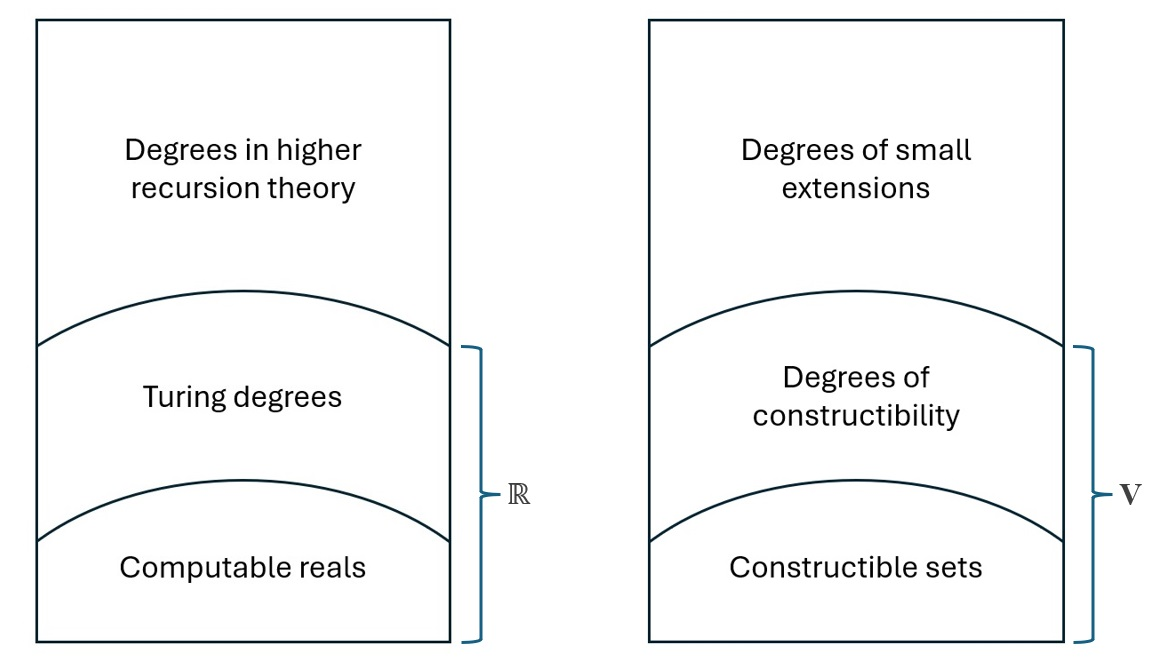
\includegraphics[width=\textwidth]{analogy.jpg}
    \captionsetup{width=0.8\textwidth, justification=centering}
    \caption{comparison between conventional notions of relative computability (left) and our generalised notions (right).}
    \label{analogy}
\end{figure}

Next, we wish to examine (necessarily non-constructive) methods of definably ``accessing'' small extensions of $V$ within $V$, or local methods in short. Set forcing is one such method, and a very well-studied one at that. In an application of set forcing, we pick a partially ordered set --- also known as a forcing notion --- $\mathbb{P} \in V$, and use a filter meeting all dense subsets of $\mathbb{P}$ in $V$ --- termed a $\mathbb{P}$-generic filter over $V$ --- to generate an extension of $V$. So the small extensions of $V$ set forcing brings about via $\mathbb{P}$ are precisely those in
\begin{equation*}
    \{V[g] : g \text{ is a } \mathbb{P} \text{-generic filter over } V\} \text{,}
\end{equation*}
a set definable outside $V$ with $\mathbb{P}$ and its dense subsets in $V$ as parameters. Consequently, one can view set forcing as a recipe in $V$ for generating small extensions of $V$ based only on parameters in $V$. The formal treatment of set forcing inspires a list of desiderata for a local method:
\begin{enumerate}[leftmargin=40pt, label=(DA\arabic*)]
    \item\label{da1} it should be definable in $V$,
    \item\label{da2} it should map parameters to descriptions of how those parameters are used to define generators of small extensions, and
    \item\label{da3} the generators it produces should depend locally on the parameters used to define them. 
\end{enumerate}

A convenient realisation at this juncture is that a recipe and its parameters (or equivalently, the two components of \ref{da2}) can be bundled up into a theory with constraints in interpretation (TCI). TCIs, already instrumental in the definition of RASMPs in Section \ref{sect2}, are basically first-order theories endowed with set constraints that may not be first-order expressible. Like standard first-order theories, TCIs admit models, and whether a set $X$ is a model of a TCI $\mathfrak{T}$ depends locally on $X$ and $\mathfrak{T}$. Defining a local method through the language of TCIs and their models thus provides immediate guarantee of \ref{da3}, and is appealing in both its brevity and robustness.

Accompanying the formalisation of local methods, ought to be a notion of relative complexity, a measure which can be utilised to check if one local method is ``more complex'' than another. Akin to relative computability, we want to define relative complexity as a transitive binary relation on the class of all local methods. There is actually a straightforward way to do this: we say method $Y$ is more complex than method $X$ iff the small extensions of $V$ picked out by $Y$ are a non-trivial refinement of those picked out by $X$. Connecting the first-order portion of a TCI with the relative complexity relation we defined, leads to the formulation of a complexity hierarchy --- the local method hierarchy --- very much in line with more notable hierarchies in theoretical computer science (e.g. the arithmetical and polynomial hierarchies).

Leveraging on a novel forcing framework developed in \cite{myself}, we are able to show that the method of set forcing is exactly $\mathsf{\Pi_2}$ in the local method hierarchy. This is the main result of Section \ref{sect3}, and it comes with two important adaptations.
\begin{enumerate}[label=(S\arabic*)]
    \item\label{s1} By applying an analogue of the Cantor-Bendixson derivative on a specific class of forcing notions, we prove that every TCI $\mathfrak{T} \in \mathsf{\Pi_2}$ either singles out $V$ or picks out continuum-many (as evaluated in the meta-theory) small extensions of $V$. The same is long known to be true for forcing notions: a trivial forcing notion gives $V$ as its sole generic extension, whereas a non-trivial one generates continuum-many generic extensions. 
    \item The main result, as well as the one in \ref{s1}, can be ported over to the context of recursion-theoretic genericity, and further strengthened. Through a closer analysis of the forcing framework of \cite{myself}, we provide an algorithm (in the conventional, Turing machine sense) that uniformly computes models of any TCI $\mathfrak{T} \in \mathsf{\Pi_2}$ from the combination of
    \begin{itemize}
        \item a real $r(\mathfrak{T})$ encoding information about $\mathfrak{T}$, and 
        \item $r(\mathfrak{T})$-$1$-generic reals.
    \end{itemize}
\end{enumerate}

\section{Relative Computability Relations on Arbitrary Sets}\label{sect2}

In this section, we progressively chip away at the very useful, but very inclusive, definition of a sequential abstract state machine to arrive at various notions of generalised (relative) computability.

\subsection{Abstract State Machines}

Gurevich introduced abstract state machines in \cite{gurevich} as general models of what we may conceptualise as an algorithm. He followed up with a number of collaborations and papers (e.g. \cite{gurevichblass}) on various subclasses of such machines. If we follow the convention of using ``algorithm'' and ``computer program'' interchangeably, then abstract state machines are natural candidates for capturing the general notion of computability. However, the claim that such machines are embodiments of algorithms seems to have undergone insufficient scrutiny. We shall start this section by refuting this claim through a set-theoretic argument. 

Briefly, a \emph{sequential abstract state machine} --- or sequential ASM (henceforth just ASM) --- $\mathfrak{M}$ comprises a class of states $S(\mathfrak{M})$, a class of initial states $I(\mathfrak{M})$, and a class transition function $\tau_{\mathfrak{M}} : S(\mathfrak{M}) \longrightarrow S(\mathfrak{M})$ such that
\begin{enumerate}[label=(A\arabic*)]
    \item\label{a1} every $s \in S(\mathfrak{M})$ is a first-order structure with the same finite signature, $\sigma(\mathfrak{M})$,
    \item\label{a2} $I(\mathfrak{M}) \subset S(\mathfrak{M})$, and
    \item\label{a3} for all $s \in S(\mathfrak{M})$, $\tau_{\mathfrak{M}}(s)$ has the same base set as $s$, and
    \item\label{a4} if $s_1, s_2 \in S(\mathfrak{M})$ and $s_1$ and $s_2$ are isomorphic, then $\tau_{\mathfrak{M}}(s_1)$ and $\tau_{\mathfrak{M}}(s_2)$ are isomorphic.
\end{enumerate}
A (finite) terminating run of $\mathfrak{M}$ is a sequence of states $(s_i : i \leq n < \omega)$ for which
\begin{enumerate}[label=(B\arabic*)]
    \item $s_0 \in I(\mathfrak{M})$,
    \item $\tau_{\mathfrak{M}}(s_n) = s_n$, and
    \item for all $m < n$, $s_{m+1} = \tau_{\mathfrak{M}}(s_m) \neq s_m$.
\end{enumerate}

For brevity's sake, some details are withheld here. First, Gurevich originally require states to have only function and constant symbols in their signatures. However, this restriction is purely cosmetic because every relation in a structure can be represented as a boolean function. Second, $\tau$ is supposed to satisfy the \emph{bounded exploration postulate}, which vaguely means that $\tau$ must perform the same updates to all states with the same interpretations of ground terms in a particular finite set. We shall keep this requirement (or at least its spirit) in mind for this subsection, even if we need not formally verify it. Finally, our definition above can be generalised so that $\tau_{\mathfrak{M}}$ need only be a binary relation -- resulting in ASMs which might not be sequential -- but that is unnecessary for the point we seek to put across.

Intuitively, a state of an ASM is a configuration of some generalised Turing machine. Each initial state corresponds to an initial configuration, from which one can read off the input (or one may take the initial state itself to be the input). The last state of a terminating run, sometimes called a \emph{final state}, corresponds in spirit to an end configuration of a Turing machine run, from which one can read off the output. For example, if we have a specific symbol $\ulcorner X \urcorner$ in the signature to represent an analogue of the Turing machine tape, then a terminating run $\Vec{r} = (s_1, \dots, s_n)$ should give an algorithmic transformation of the input representation $X^{s_1}$ into the output representation $X^{s_n}$.

We argue against ASMs as a good notion of generalised algorithms. Consider the example below.

\begin{ex}\label{ex21}
Let $\kappa$ be an infinite cardinal. Expand the signature of $(\kappa; \in)$ to include a unary relation symbol $\ulcorner A \urcorner$ and a constant symbol $\ulcorner c \urcorner$. Now if $A_1$ and $A_2$ are subsets of $\kappa$, then we can define a sequential ASM $\mathfrak{M}(\kappa, A_1, A_2)$ as follows:
\begin{gather*}
    s_1 := (\kappa; \in, A_1, 0) \\
    s_2 := (\kappa; \in, A_2, 1) \\
    S(\mathfrak{M}(\kappa, A_1, A_2)) := \{s_1, s_2\} \\
    I(\mathfrak{M}(\kappa, A_1, A_2)) := \{s_1\} \\
    \tau_{\mathfrak{M}(\kappa, A_1, A_2)} := \{(s_1, s_2), (s_2, s_2)\} \text{.}
\end{gather*}
Observe that $A_1$ and $A_2$ both interpret $\ulcorner A \urcorner$ on the base set $\kappa$, and that $s_1$ is not isomorphic to $s_2$ because 
\begin{itemize}
    \item $s_1$ interprets $\ulcorner c \urcorner$ as $0$ and $s_2$ interprets $\ulcorner c \urcorner$ as $1$, and
    \item there is no automorphism of $(\kappa; \in)$ other than the identity on $\kappa$.
\end{itemize}
This means $S(\mathfrak{M}(\kappa, A_1, A_2))$, $I(\mathfrak{M}(\kappa, A_1, A_2))$ and $\tau_{\mathfrak{M}(\kappa, A_1, A_2)}$ satisfy \ref{a1} to \ref{a4} in place of $S(\mathfrak{M})$, $I(\mathfrak{M})$ and $\tau_{\mathfrak{M}}$ respectively. Furthermore, $c$ is specifically added to the signature so that the finite set $\{c\}$ witnesses $\mathfrak{M}(\kappa, A_1, A_2)$ satisfy the bounded exploration postulate.
\end{ex}

Fix subsets $A_1$ and $A_2$ of $\kappa$. The only terminating run of $\mathfrak{M}(\kappa, A_1, A_2)$ is $(s_1, s_2)$. Morally, this is saying that we can algorithmically get from $A_1$ to $A_2$. If we set $A_1$ to be a simply definable set like the empty set, then every subset of $\kappa$ is algorithmically derivable from $A_1$. This seems incredible given the information content of arbitrary sets of ordinals, as exemplified by the next proposition.

\begin{prop}\label{prop22}
Let $M$ be a transitive model of $\mathsf{ZFC}$ and $X \in M$. Then there is a set of ordinals $c \in M$ such that if $N$ is any transitive model of $\mathsf{ZFC}$ containing $c$, then $X \in N$. 
\end{prop}

\begin{proof}
Let $Y'$ be the transitive closure of $X$ (under the membership relation $\in$) and set $Y := Y' \cup \{X\}$. Then $Y$ is $\in$-transitive. Choose a bijection $f$ from a cardinal $\kappa$ into $Y$. Use $\in'$ to denote the unique binary relation $R$ on $\kappa$ such that
\begin{equation*}
    R(\alpha, \beta) \iff f(\alpha) \in f(\beta) \text{.}
\end{equation*}
Now apply G\"{o}del's pairing function to code $\in'$ as a subset $c$ of $\kappa$. To recover $X$ from $c$, first apply the inverse of the pairing function followed by the Mostowski collapse to get $Y$. Then $X$ is definable from $Y$ as the unique $\in$-maximal element of $Y$. This decoding process is absolute for transitive models of $\mathsf{ZFC}$ because all its components are.
\end{proof}

Proposition \ref{prop22} allows us to code any set as a set of ordinals such that the decoding can be done in an absolute manner. If we believe that such a decoding scheme (particularly, G\"{o}del's pairing function) is algorithmic, then the definition of ASMs entails that we can algorithmically derive every set in $V$ from just $\emptyset$. Since most set theorists are of the opinion that sets in $V$ can be extremely complicated and far from constructible in a very strong sense, this conclusion is wholly unsatisfactory, if not patently false. In other words, ASMs are \emph{too} encompassing a paradigm for algorithms, and thus should not be used to draw the line for generalised computability.

For much of the rest of this section, we will make educated modifications to the definition of an ASM, in an attempt to formulate a philosophically justified notion of algorithms.

\subsection{Modifying the Satisfaction Relation}

An obvious cause of the triviality identified in the preceding paragraph, is the lack of restriction on the transition function $\tau_{\mathfrak{M}}$ of an ASM $\mathfrak{M}$. Ideally, $\tau_{\mathfrak{M}}(s)$ should be describable is a way which only depends locally on itself and $s$. One formalisation of a ``describable local property'' applicable to first-order structures is the notion of a \emph{first-order property}. A first-order formula $\phi$ over the signature of a structure $\mathfrak{A}$ is a first-order property of $\mathfrak{A}$ iff $\mathfrak{A} \models \phi$, where $\models$ is Tarski's satisfaction relation. However, in our use case, the formula $\phi$ might need to refer to two different structures, so some slight modifications to the satisfaction relation are in order.

\begin{defi}
Given an signature $\sigma$, define $2 \cdot \sigma$ to be the disjoint union of $\sigma$ and itself. In other words, for each symbol $\ulcorner X \urcorner \in \sigma$ and each $i < 2$, we choose a fresh symbol $\ulcorner X_{i} \urcorner$ and cast it to be of the same type and arity as $\ulcorner X \urcorner$. We then set
\begin{equation*}
    2 \cdot \sigma := \{\ulcorner X_{i} \urcorner : \ulcorner X \urcorner \in \sigma \text{ and } i < 2\} \text{.}
\end{equation*}
\end{defi}

\begin{defi}
A \emph{binary first-order formula} over a signature $\sigma$ is a first-order formula over $2 \cdot \sigma$.
\end{defi}

\begin{defi}
Let $\mathfrak{A}_0$ and $\mathfrak{A}_1$ be first-order structures with the same base set $A$ and signature $\sigma$. For each $a \in A$, choose a fresh constant symbol $\ulcorner a \urcorner$ not in $2 \cdot \sigma$. Denote
\begin{equation*}
    2 \cdot \sigma \cup \{\ulcorner a \urcorner : a \in A\}
\end{equation*}
as $\sigma(A, 2)$.
\end{defi}

\begin{defi}
Let $\mathfrak{A}_0$ and $\mathfrak{A}_1$ be first-order structures with the same base set $A$ and signature $\sigma$. Let $\ulcorner X \urcorner \in \sigma(A, 2)$.
Define
\begin{itemize}
    \item $X^{(\mathfrak{A}_0, \mathfrak{A}_1)} := a$ if $\ulcorner X \urcorner = \ulcorner a \urcorner$ for some $a \in A$,
    \item $X^{(\mathfrak{A}_0, \mathfrak{A}_1)} := Y^{\mathfrak{A}_0}$ if $\ulcorner X \urcorner = \ulcorner Y_0 \urcorner$ for some $\ulcorner Y \ulcorner \in \sigma$, and
    \item $X^{(\mathfrak{A}_0, \mathfrak{A}_1)} := Y^{\mathfrak{A}_1}$ if $\ulcorner X \urcorner = \ulcorner Y_1 \urcorner$ for some $\ulcorner Y \ulcorner \in \sigma$.
\end{itemize}
If $\ulcorner f \urcorner \in \sigma(A, 2)$ is a function symbol and $t$ is a term over $\sigma(A, 2)$ of which interpretation under $(\mathfrak{A}_0, \mathfrak{A}_1)$ is known, then 
\begin{equation*}
    f(t)^{(\mathfrak{A}_0, \mathfrak{A}_1)} := f^{(\mathfrak{A}_0, \mathfrak{A}_1)}(t^{(\mathfrak{A}_0, \mathfrak{A}_1)}) \text{.}
\end{equation*}
\end{defi}

\begin{defi}
Let $\mathfrak{A}_0$ and $\mathfrak{A}_1$ be first-order structures with the same base set $A$ and signature $\sigma$. We define what $(\mathfrak{A}_0, \mathfrak{A}_1) \models_2 \phi$ means for $\phi \in \sigma(A, 2)$ by recursion on the complexity of $\phi$.
\begin{itemize}
    \item If $\phi = \ulcorner t_1 = t_2 \urcorner$ for terms $t_1, t_2$ over $\sigma(A, 2)$, then $$(\mathfrak{A}_0, \mathfrak{A}_1) \models_2 \phi \text{ iff } t_1^{(\mathfrak{A}_0, \mathfrak{A}_1)} = t_2^{(\mathfrak{A}_0, \mathfrak{A}_1)} \text{.}$$
    \item If $\phi = \ulcorner R(t_1, \dots, t_n) \urcorner$ for a relation symbol $\ulcorner R \urcorner \in \sigma(A, 2)$ and terms $t_1, \dots, t_n$ over $\sigma(A, 2)$, then $$(\mathfrak{A}_0, \mathfrak{A}_1) \models_2 \phi \text{ iff } R^{(\mathfrak{A}_0, \mathfrak{A}_1)} (t_1^{(\mathfrak{A}_0, \mathfrak{A}_1)}, \dots, t_n^{(\mathfrak{A}_0, \mathfrak{A}_1)}) \text{.}$$
    \item If $\phi = \ulcorner \neg \psi \urcorner$ for a formula $\psi$ over $\sigma(A, 2)$, then $$(\mathfrak{A}_0, \mathfrak{A}_1) \models_2 \phi \text{ iff } \neg ((\mathfrak{A}_0, \mathfrak{A}_1) \models_2 \psi) \text{.}$$
    \item If $\phi = \ulcorner \psi_1 \wedge \psi_2 \urcorner$ for formulas $\psi_1$ and $\psi_2$ over $\sigma(A, 2)$, then $$(\mathfrak{A}_0, \mathfrak{A}_1) \models_2 \phi \text{ iff } ((\mathfrak{A}_0, \mathfrak{A}_1) \models_2 \psi_1 \wedge (\mathfrak{A}_0, \mathfrak{A}_1) \models_2 \psi_2) \text{.}$$
    \item If $\phi = \ulcorner \exists x \ \psi \urcorner$ for a free variable $\ulcorner x \urcorner$ and a formula $\psi$ over $\sigma(A, 2)$, then $$(\mathfrak{A}_0, \mathfrak{A}_1) \models_2 \phi \text{ iff } \exists a \in A ((\mathfrak{A}_0, \mathfrak{A}_1) \models_2 \psi[x \mapsto a]) \text{,}$$ where $\psi[x \mapsto a]$ is the result of replacing all instances of $\ulcorner x \urcorner$ in $\psi$ by $\ulcorner a \urcorner$.
\end{itemize}
\end{defi}

Before adding more requirements to the transition function of an ASM, let us enforce that every state in an ASM $\mathfrak{M}$ must have the same base set $b(\mathfrak{M})$. This can be done without loss of generality in the original definition of an ASM, because we can extend the base set of each state in $\mathfrak{M}$ to be the union of the base sets of states in $\mathfrak{M}$, while arbitrarily extending the interpretation of function and relation symbols in the signature by each state.

We stipulate that the transition function $\tau_{\mathfrak{M}}$ of an ASM $\mathfrak{M}$ must be finitely describable over $2 \cdot \sigma(\mathfrak{M})$. That is, there must exist a first-order sentence $\phi^{\tau}_{\mathfrak{M}}$ over $2 \cdot \sigma(\mathfrak{M})$ such that for all $s_1, s_2 \in S(\mathfrak{M})$, 
\begin{equation*}
    \tau_{\mathfrak{M}}(s_1) = s_2 \iff (s_1, s_2) \models_2 \phi^{\tau}_{\mathfrak{M}} \text{.}
\end{equation*}

This new imposition on transition functions seems sufficiently severe to rule out the cases in Example \ref{ex21}. Or does it?

\begin{ex}[\ref{ex21} revisited]
Let $\kappa$, $A_1$, $A_2$, $s_1$, $s_2$ and $\mathfrak{M}(\kappa, A_1, A_2)$ be as in Example \ref{ex21}. Set 
\begin{gather*}
    \phi^{\tau}_{\mathfrak{M}(\kappa, A_1, A_2)} := \ulcorner \forall x \ (x \in_1 c_1 \iff (\forall y \ (\neg (y \in_1 x)))) \urcorner \text{.}
\end{gather*}
Then given any two expansions $s'_1$ and $s'_2$ of $(\kappa; \in)$ with signature $\sigma$ containing $\ulcorner c \urcorner$, 
\begin{equation*}
    (s'_1, s'_2) \models_2 \phi^{\tau}_{\mathfrak{M}(\kappa, A_1, A_2)} \text{ iff } s'_2 \text{ interprets } \ulcorner c \urcorner \text{ to be } 1 \text{.}
\end{equation*}
In particular, $(s_1, s_2) \models_2 \phi^{\tau}_{\mathfrak{M}(\kappa, A_1, A_2)}$ and $(s_2, s_2) \models_2 \phi^{\tau}_{\mathfrak{M}(\kappa, A_1, A_2)}$, so $\tau_{\mathfrak{M}(\kappa, A_1, A_2)}$ is still a valid transition function. 
\end{ex}

It turns out that we can intentionally choose the set of states in an ASM to trivialise the definition of its transition function. To overcome this, we make it so that the set of states depends only on the base set and signature of the structures involved. What this means is, if $\mathfrak{M}_1$ and $\mathfrak{M}_2$ are ASMs, $s_1 \in S(\mathfrak{M}_1)$, $s_2 \in S(\mathfrak{M}_2)$ and $s_1$, $s_2$ share the same base set and signature, then $S(\mathfrak{M}_1) = S(\mathfrak{M}_2)$. To wit, we include $b(\mathfrak{M})$ as a primary datum of an ASM, and derive $S(\mathfrak{M})$ from $b(\mathfrak{M})$ and $\sigma(\mathfrak{M})$ as follows: 
\begin{equation*}
    S(\mathfrak{M}) := \{s : s \text{ is a first-order structure with base set } b(\mathfrak{M}) \text{ and signature } \sigma(\mathfrak{M})\} \text{.}
\end{equation*}

Now, there may be a nagging worry that we over-corrected, that our modified definition of an ASM is too restrictive. Indeed, this shortcoming becomes obvious when we try to define an ASM corresponding to a Turing machine.

\begin{diff}\label{diff29}
Consider a Turing machine $M$ with an $\omega$-length tape and $n$ states, for some $n < \omega$. An ASM $\mathfrak{M}$ representing $M$ naturally has $b(\mathfrak{M})$ include $\omega$ and the set of $M$'s states. A suitable transition function $\tau_{\mathfrak{M}}$ ought to speak of $M$'s states, and to do that it is imperative that each of these states identify uniquely with a term over $\sigma(\mathfrak{M})$. For example, we can have a constant symbol $\ulcorner c_i \urcorner \in \sigma(\mathfrak{M})$ uniquely represent the $i$-th state of $M$. 

However, as members of $S(\mathfrak{M})$ are allowed to freely interpret the $\ulcorner c_i \urcorner$s, there would be a problem of singling out the ``next state'' of $\mathfrak{M}$ based on an arbitrary ``current state'', using the relation $\models_2$ alone.
\end{diff}

Difficulty \ref{diff29} tells us $S(\mathfrak{M})$ should depend not just on $b(\mathfrak{M})$ and $\sigma(\mathfrak{M})$, but also on how symbols in $\sigma(\mathfrak{M})$ are to be interpreted in $b(\mathfrak{M})$. This leads us to the objects of focus in the next subsection.

\subsection{Theories with Constraints in Interpretation}\label{ssect23}

\emph{Theories with constraints in interpretation} (henceforth, \emph{TCI}s) were conceived in \cite{myself} as a convenient means of looking at generic objects produced by set-theoretic forcing. Their utility in that respect will be clearer in the next section. Nevertheless, we introduce them here so that they can be used to constrain the possible states of an ASM. 

\begin{defi}(Lau, \cite{myself})
A \emph{first-order theory with constraints in interpretation} (\emph{first-order TCI}) --- henceforth, just \emph{theory with constraints in interpretation} (\emph{TCI}) --- is a tuple $(T, \sigma, \dot{\mathcal{U}}, \vartheta)$, where
\begin{itemize}
    \item $T$ is a first order theory with signature $\sigma$,
    \item $\dot{\mathcal{U}}$ is a unary relation symbol not in $\sigma$,
    \item $\vartheta$ is a function (the \emph{interpretation constraint map}) with domain $\sigma \cup \{\dot{\mathcal{U}}\}$, 
    \item if $x \in ran(\vartheta)$, then there is $y$ such that 
    \begin{itemize}[label=$\circ$]
        \item either $x = (y, 0)$ or $x = (y, 1)$, and
        \item if $\vartheta(\dot{\mathcal{U}}) = (z, a)$, then $y \subset z^n$ for some $n < \omega$, and
    \end{itemize}
    \item if $\vartheta(\dot{\mathcal{U}}) = (z, a)$, then 
    \begin{itemize}[label=$\circ$]
        \item $z \cap z^n = \emptyset$ whenever $1 < n < \omega$, and
        \item $z^m \cap z^n = \emptyset$ whenever $1 < m < n < \omega$.
    \end{itemize}
\end{itemize}
\end{defi}

We call members of the interpretation constraint map \emph{interpretation constraints}.

\begin{defi}(Lau, \cite{myself})
Let $(T, \sigma, \dot{\mathcal{U}}, \vartheta)$ be a TCI. We say $\mathcal{M} := (U; \mathcal{I}) \models^* (T, \sigma, \dot{\mathcal{U}}, \vartheta)$ --- or $\mathcal{M}$ \emph{models} $(T, \sigma, \dot{\mathcal{U}}, \vartheta)$ --- iff all of the following holds:
\begin{itemize}
    \item $\mathcal{M}$ is a structure,
    \item $\sigma$ is the signature of $\mathcal{M}$,
    \item $\mathcal{M} \models T$,
    \item if $\vartheta(\dot{\mathcal{U}}) = (y, 0)$, then $U \subset y$,
    \item if $\vartheta(\dot{\mathcal{U}}) = (y, 1)$, then $U = y$, and
    \item for $\dot{X} \in \sigma$,
    \begin{itemize}[label=$\circ$]
        \item if $\dot{X}$ is a constant symbol and $\vartheta(\dot{X}) = (y, z)$, then $\mathcal{I}(\dot{X}) \in y \cap U$,
        \item if $\dot{X}$ is an $n$-ary relation symbol and $\vartheta(\dot{X}) = (y, 0)$, then $\mathcal{I}(\dot{X}) \subset y \cap U^{n}$,
        \item if $\dot{X}$ is an $n$-ary relation symbol and $\vartheta(\dot{X}) = (y, 1)$, then $\mathcal{I}(\dot{X}) = y \cap U^{n}$,
        \item if $\dot{X}$ is an $n$-ary function symbol and $\vartheta(\dot{X}) = (y, 0)$, then $$\{z \in U^{n+1} : \mathcal{I}(\dot{X})(z \! \restriction_n) = z(n)\} \subset y \cap U^{n+1}, \text{ and}$$
        \item if $\dot{X}$ is an $n$-ary function symbol and $\vartheta(\dot{X}) = (y, 1)$, then $$\{z \in U^{n+1} : \mathcal{I}(\dot{X})(z \! \restriction_n) = z(n)\} = y \cap U^{n+1}.$$
    \end{itemize}
\end{itemize}
We say $(T, \sigma, \dot{\mathcal{U}}, \vartheta)$ has a model if there exists $\mathcal{M}$ for which $\mathcal{M} \models^* (T, \sigma, \dot{\mathcal{U}}, \vartheta)$.
\end{defi}

To specify an ASM $\mathfrak{M}$, we should also specify a TCI $\mathfrak{T}(\mathfrak{M}) = (T, \sigma, \dot{\mathcal{U}}, \vartheta)$ such that 
\begin{gather*}
    T = \emptyset \\
    \sigma = \sigma(\mathfrak{M}) \\
    \vartheta(\dot{\mathcal{U}}) = (b(\mathfrak{M}), 1).
\end{gather*}
We can then stipulate that 
\begin{equation*}
    S(\mathfrak{M}) := \{s : s \models^* \mathfrak{T}(\mathfrak{M})\} \text{.}
\end{equation*}

Let us now check that any Turing machine can be easily represented as an ASM.

\begin{ex}\label{ex212}
As in Difficulty \ref{diff29}, let $M$ be a Turing machine with an $\omega$-length tape and $n$ states, for some $0 < n < \omega$. Let the set of $M$'s states be $\{c_i : i < n\}$, with $c_0$ being the only initial state and $c_{n-1}$ the only final state. 

Choose a binary relation symbol $\ulcorner \in \urcorner$, unary relation symbols $\dot{\mathcal{U}}$, $\ulcorner R \urcorner$, unary function symbols $\ulcorner \mathrm{Pre} \urcorner$, $\ulcorner \mathrm{Suc} \urcorner$, and constant symbols $\ulcorner h \urcorner$, $\ulcorner t \urcorner$, all of them distinct from one another. Set 
\begin{gather*}
    b(\mathfrak{M}) := \omega \\
    \sigma(\mathfrak{M}) := \{\ulcorner \in \urcorner, \ulcorner \mathrm{Pre} \urcorner, \ulcorner \mathrm{Suc} \urcorner, \ulcorner h \urcorner, \ulcorner t \urcorner, \ulcorner R \urcorner\} \text{.}
\end{gather*}
Define a function $\vartheta$ on $\sigma(\mathfrak{M}) \cup \{\dot{\mathcal{U}}\}$ as follows:
\begin{gather*}
    \vartheta(\dot{\mathcal{U}}) := (\omega, 1) \\
    \vartheta(\ulcorner \in \urcorner) := (\in \cap \ \omega, 1) \\
    \vartheta(\ulcorner \mathrm{Pre} \urcorner) := (\mathrm{Pre}, 1) \\
    \vartheta(\ulcorner \mathrm{Suc} \urcorner) := (\mathrm{Suc}, 1) \\
    \vartheta(\ulcorner h \urcorner) := (\omega, 0) \\
    \vartheta(\ulcorner t \urcorner) := (\omega, 0) \\
    \vartheta(\ulcorner R \urcorner) := (\omega, 0) \text{,}
\end{gather*}
where $\mathrm{Pre}$ and $\mathrm{Suc}$ are the predecessor and successor functions on $\omega$, respectively. Set
\begin{equation*}
    \mathfrak{T}(\mathfrak{M}) := (\emptyset, \sigma(\mathfrak{M}), \dot{\mathcal{U}}, \vartheta) \text{.}
\end{equation*}
Intuitively, we want $\ulcorner h \urcorner$ to interpret the current position of the read/write head of $M$, $\ulcorner t \urcorner$ to interpret the current state $M$ is in, and $\ulcorner R \urcorner$ to interpret the current contents of $M$'s tape. Notice that all members of $\omega$ are definable over the membership  relation without parameters. This implies references to them can be made in sentences over $\sigma(\mathfrak{M})$. We will use $\langle n \rangle$ to refer to the $n < \omega$ in such sentences. 

Define 
\begin{align*}
    I(\mathfrak{M}) := \{s : & s \models^* \mathfrak{T}(\mathfrak{M}) \text{ and } \\
    & s \models \ulcorner h = \langle 0 \rangle \wedge t = \langle 0 \rangle \urcorner \text{ and } \\
    & s \models \ulcorner \exists x \ (R(x)) \wedge \forall x \ \forall y \ (R(x) \wedge R(y) \implies x = y) \urcorner\} \text{.}
\end{align*}
Each member of $I(\mathfrak{M})$ represents an initial configuration of $M$ with the read/write head at the $0$-th cell of the tape, the current state being the initial state, and `$1$' written on exactly one cell of the tape. More specifically, `$1$' appears on the $k$-th cell of $M$'s tape in an initial configuration iff $M$ takes $k$ as input.

We are almost done with specifying our ASM $\mathfrak{M}$; the only thing left to do is to give a transition function $\tau_{\mathfrak{M}}$ accurately representing transitions among the Turing configurations of $M$. It suffices to concoct a suitable sentence $\phi^{\tau}_{\mathfrak{M}}$ based on the transition function $$\delta : \{c_i : i < n-1\} \times 2 \longrightarrow \{c_i : i < n\} \times 2 \times \{\mathrm{left}, \mathrm{right}\}$$ of $M$. For each pair $(j, k) \in n \times 2$, let
\begin{align*}
    \phi_{j,k} := \ & \ulcorner (q(R_0(h_0), k) \wedge t_0 \! = \! \langle j \rangle) \!\! \implies \!\! (q(R_1(h_0), k') \wedge t_1 \! = \! \langle j' \rangle \wedge h_1 \! = \mathrm{Pre}(h_0) \wedge \varphi) \urcorner \\ 
    & \text{ if } j < n-1 \text{ and } \delta((c_j, k)) = (c_{j'}, k', \mathrm{left}) \text{,} \\
    \phi_{j,k} := \ & \ulcorner (q(R_0(h_0), k) \wedge t_0 \! = \! \langle j \rangle) \!\! \implies \!\! (q(R_1(h_0), k') \wedge t_1 \! = \! \langle j' \rangle \wedge h_1 \! = \mathrm{Suc}(h_0) \wedge \varphi) \urcorner \\ 
    & \text{ if } j < n-1 \text{ and } \delta((c_j, k)) = (c_{j'}, k', \mathrm{right}) \text{, and} \\
    \phi_{j,k} := \ & \ulcorner h_0 = h_1 \wedge t_0 = t_1 \wedge \forall x \ (R_0(x) \iff R_1(x)) \urcorner \\ 
    & \text{ if } j = n-1 \text{,}
\end{align*}
where $q(\psi, k)$ is a shorthand for 
\begin{align*}
    \neg \psi & \text{ if } k = 0 \text{;} \\
    \psi & \text{ if } k = 1
\end{align*}
and $\varphi$ is the sentence
\begin{equation*}
    \ulcorner \forall x \ (\neg x = h_0 \implies (R_0(x) \iff R_1(x))) \urcorner \text{.}
\end{equation*}
Finally, 
\begin{equation*}
    \phi^{\tau}_{\mathfrak{M}} := \bigwedge \{\phi_{j,k} : (j, k) \in n \times 2\} \text{,}
\end{equation*}
is a first-order sentence over $2 \cdot \sigma(\mathfrak{M})$ that gives us the representation we want.
\end{ex}

\subsection{Absoluteness and the Bounded Exploration Postulate}

A good notion of algorithm ought to be absolute to a certain degree. In set-theoretic contexts, absoluteness for transitive models of set theory comes up the most often. 

\begin{defi}
A sentence $\phi$ in the language of set theory with set parameters is \emph{absolute for transitive models of} $\mathsf{ZFC}$ iff for all $A$ and $B$ such that
\begin{itemize}
    \item $A \subset B$,
    \item $(A; \in)$ and $(B; \in)$ are transitive models of $\mathsf{ZFC}$, and
    \item all parameters of $\phi$ are members of $A$,
\end{itemize}
\begin{equation*}
    (A; \in) \models \phi \iff (B; \in) \models \phi \text{.}
\end{equation*}
\end{defi}

\begin{defi}
Let $\phi$ be a formula in the language of set theory, with set parameters and free variables $x_1, \dots, x_n$. Suppose $\phi$ defines an $n$-ary relation $R$ (in $V$). Then $\phi$ is an \emph{absolute definition of} (or, $\phi$ \emph{absolutely defines}) $R$ \emph{for transitive models of} $\mathsf{ZFC}$ iff for all $A$ such that
\begin{itemize}
    \item $(A; \in)$ is a transitive model of $\mathsf{ZFC}$, and
    \item all parameters of $\phi$ are members of $A$,
\end{itemize}
\begin{equation*}
     \{(a_1, \dots, a_n) \in A^n : (A; \in) \models \phi[x_1 \mapsto a_1, \dots, x_n \mapsto a_n]\} = R \cap A \text{.}
\end{equation*}
\end{defi}

Recall that it is implicit in our modified definition of an ASM $\mathfrak{M}$, that $\phi^{\tau}_{\mathfrak{M}}$ needs to have the following property:
\begin{equation}\label{eq1}
    \forall s_0 \in S(\mathfrak{M}) \ \exists ! s_1 \in S(\mathfrak{M}) \ ((s_0, s_1) \models_2 \phi^{\tau}_{\mathfrak{M}}) \text{,}
\end{equation}
where
\begin{equation*}
    S(\mathfrak{M}) = \{s : s \models^* \mathfrak{T}(\mathfrak{M})\} \text{.}
\end{equation*}
However, given any $\mathfrak{T}(\mathfrak{M})$ and $\phi^{\tau}_{\mathfrak{M}}$, it is not immediate that (\ref{eq1}) is absolute for transitive models of $\mathsf{ZFC}$. As a result, it is difficult to ascertain that the definition of $\tau_{\mathfrak{M}}$ from $\mathfrak{T}(\mathfrak{M})$ and $\phi^{\tau}_{\mathfrak{M}}$ is absolute for transitive models of $\mathsf{ZFC}$. This implores us to make the dependency between the current and the next state of an ASM even more local.

At this point, it is useful to make precise Gurevich's bounded exploration postulate, for it is an example of highly local dependency. Combined with our stipulation that a transition function must be definable, we expect to obtain a level of local definability from which the absoluteness we want can be easily derived. Consequently, abiding by the bounded exploration postulate should net us absoluteness at no additional cost.

\begin{defi}
Let $\mathfrak{M}$ be an ASM and $s \in S(\mathfrak{M})$. Define $\Delta_{\mathfrak{M}}(s)$ to be the unique function from $\sigma(\mathfrak{M})$ into $\mathcal{P}(b(\mathfrak{M}))$ such that
\begin{itemize}
    \item if $\ulcorner X \urcorner \in \sigma(\mathfrak{M})$ is an $n$-ary function symbol, then 
    \begin{equation*}
        \Delta_{\mathfrak{M}}(s)(\ulcorner X \urcorner) = \{\Vec{z} \in b(\mathfrak{M})^n : \ulcorner X \urcorner^{s}(\Vec{z}) \neq \ulcorner X \urcorner^{\tau_{\mathfrak{M}}(s)}(\Vec{z})\} \text{,}
    \end{equation*}
    \item if $\ulcorner X \urcorner \in \sigma(\mathfrak{M})$ is an $n$-ary relation symbol, then 
    \begin{equation*}
        \Delta_{\mathfrak{M}}(s)(\ulcorner X \urcorner) = \{\Vec{z} \in b(\mathfrak{M})^n : \neg (\ulcorner X \urcorner^{s}(\Vec{z})) \iff \ulcorner X \urcorner^{\tau_{\mathfrak{M}}(s)}(\Vec{z})\} \text{,}
    \end{equation*}
    \item if $\ulcorner X \urcorner \in \sigma(\mathfrak{M})$ is a constant symbol, then 
    \begin{equation*}
        \Delta_{\mathfrak{M}}(s)(\ulcorner X \urcorner) =
        \begin{cases}
            \emptyset & \text{if } \ulcorner X \urcorner^{s} = \ulcorner X \urcorner^{\tau_{\mathfrak{M}}(s)} \\
            b(\mathfrak{M}) & \text{otherwise.}
        \end{cases}
    \end{equation*}
\end{itemize}
Note that if $b(\mathfrak{M}) = \emptyset$, then $S(\mathfrak{M})$ is a singleton and for every $s \in S(\mathfrak{M})$, $\tau_{\mathfrak{M}}(s) = s$. Necessarily, any such $\mathfrak{M}$ must have $\Delta_{\mathfrak{M}}(s_0) = \Delta_{\mathfrak{M}}(s_1)$ for all $s_0, s_1 \in S(\mathfrak{M})$.
\end{defi}

\begin{defi}
Let $\mathfrak{M}$ be an ASM. Its transition function $\tau_{\mathfrak{M}}$ satisfies the \emph{bounded exploration postulate} iff there is a finite set of ground terms $\mathcal{D}$ over $\sigma(\mathfrak{M})$ such that for all $\ulcorner X \urcorner \in \sigma(\mathfrak{M})$ and $s_0, s_1 \in S(\mathfrak{M})$,
\begin{equation*}
    \forall t \in \mathcal{D} \ (t^{s_0} = t^{s_1}) \implies \Delta_{\mathfrak{M}}(s_0) = \Delta_{\mathfrak{M}}(s_1) \text{.}
\end{equation*}
\end{defi}

As every relation is a boolean function, there is a canonical way of simulating relation symbols in a ground term. Thus from a computability point of view, the bounded exploration postulate seems intuitive enough at first glance. Upon closer inspection, however, the emphasis on changes in valuations gives rise to artefacts such as the one below.

\begin{ex}
Consider ASMs $\mathfrak{M}_1$ and $\mathfrak{M}_2$ such that 
\begin{gather*}
    \sigma(\mathfrak{M}_1) = \sigma(\mathfrak{M}_2) = \{\ulcorner \mathrm{In} \urcorner, \ulcorner \mathrm{Out} \urcorner\} \\
    \mathfrak{T}(\mathfrak{M}_1) = \mathfrak{T}(\mathfrak{M}_2) \text{,}
\end{gather*}
$b(\mathfrak{M}_1)$ is infinite, and
\begin{gather*}
    \phi^{\tau}_{\mathfrak{M}_1} = \ulcorner \forall x \ ((\mathrm{In}_1(x) \iff \neg \mathrm{In}_0(x)) \wedge (\mathrm{Out}_1(x) \iff \neg \mathrm{Out}_0(x))) \urcorner \\
    \phi^{\tau}_{\mathfrak{M}_2} = \ulcorner \forall x \ ((\mathrm{In}_1(x) \iff x \neq x) \wedge (\mathrm{Out}_1(x) \iff \mathrm{Out}_0(x))) \urcorner \text{.}
\end{gather*}
Here, $\ulcorner \mathrm{In} \urcorner$ and $\ulcorner \mathrm{Out} \urcorner$ are supposed to represent input and output tapes respectively, with cells indexed by $b(\mathfrak{M}_1) = b(\mathfrak{M}_2)$ and entries from a binary alphabet. $\tau_{\mathfrak{M}_1}$ flips each bit of the input and output tapes, whereas $\tau_{\mathfrak{M}_2}$ resets the input tape to its all-zeroes state, an operation one can think of as a complete erasure of input tape data.

Observe that $\tau_{\mathfrak{M}_1}$ satisfies the bounded exploration postulate because for all $s_0, s_1 \in S(\mathfrak{M}_1)$, 
\begin{equation*}
    \Delta_{\mathfrak{M}}(s_0) = \Delta_{\mathfrak{M}}(s_1) = \{(\ulcorner \mathrm{In} \urcorner, b(\mathfrak{M}_1)), (\ulcorner \mathrm{Out} \urcorner, b(\mathfrak{M}_1))\} \text{.}
\end{equation*}
On the other hand, $\tau_{\mathfrak{M}_2}$ does not satisfy the bounded exploration postulate because for $s_0, s_1 \in S(\mathfrak{M}_1)$, $\Delta_{\mathfrak{M}}(s_0) = \Delta_{\mathfrak{M}}(s_1)$ only if $\ulcorner \mathrm{In} \urcorner^{s_0} = \ulcorner \mathrm{In} \urcorner^{s_1}$, and whether $\ulcorner \mathrm{In} \urcorner^{s_0} = \ulcorner \mathrm{In} \urcorner^{s_1}$ cannot be determined by just examining a finite fragment of $s_0$ and a finite fragment of $s_1$. This means the transition function of any ASM built on $\tau_{\mathfrak{M}_2}$ by enlarging its signature while maintaining its function (``erase all data from the input tape and do nothing else''), cannot possibly satisfy the postulate.

We hence find ourselves in a weird position whereby universal bit-flipping --- which requires some information of prior states --- is an acceptably bounded, but universal erasure --- which requires no prior knowledge --- is not.
\end{ex}

Besides the erasure of a tape's contents, one would expect the copying of one tape's contents to another to be as valid a step as universal bit-flipping. We seek to reformulate the bounded exploration postulate with these in mind.

\begin{defi}\label{def220}
Let $\sigma$ be a signature. We say a sentence $\phi$ over $2 \cdot \sigma$ is \emph{bounded for} $\sigma$ iff for each $\ulcorner X \urcorner \in \sigma$ there are $\phi^{\ulcorner X \urcorner}$ and $\psi^{\ulcorner X \urcorner}$ such that
\begin{itemize}
    \item $\phi^{\ulcorner X \urcorner}$ is a formula over $\{\ulcorner Y_0 \urcorner : \ulcorner Y \urcorner \in \sigma\}$ ($\subset 2 \cdot \sigma$),
    \item $\psi^{\ulcorner X \urcorner}$ is a sentence over $2 \cdot \sigma$,
    \item if $\ulcorner X \urcorner$ is an $n$-ary function symbol, then 
    \begin{itemize}[label=$\circ$, leftmargin=20pt]
        \item $\phi^{\ulcorner X \urcorner}$ contains $n + 1$ free variables, and
        \item for some variable symbols $y_1, \dots, y_{n+1}$,
        \begin{align*}
            \psi^{\ulcorner X \urcorner} = \ulcorner \forall y_1 \dots \forall y_{n+1} \ (X_1(y_1, \dots, y_n) = y_{n+1} \iff \phi^{\ulcorner X \urcorner}(y_1, \dots, y_{n+1})) \urcorner \text{,}
        \end{align*}
    \end{itemize}
    \item if $\ulcorner X \urcorner$ is an $n$-ary relation symbol, then 
    \begin{itemize}[label=$\circ$, leftmargin=20pt]
        \item $\phi^{\ulcorner X \urcorner}$ contains $n$ free variables, and
        \item for some variable symbols $y_1, \dots, y_n$,
        \begin{align*}
            \psi^{\ulcorner X \urcorner} = \ulcorner \forall y_1 \dots \forall y_n \ (X_1(y_1, \dots, y_n) \iff \phi^{\ulcorner X \urcorner}(y_1, \dots, y_n)) \urcorner \text{,}
        \end{align*}
    \end{itemize}
    \item if $\ulcorner X \urcorner$ is a constant symbol, then 
    \begin{itemize}[label=$\circ$, leftmargin=20pt]
        \item $\phi^{\ulcorner X \urcorner}$ contains $1$ free variable, and
        \item for some variable symbol $y$,
        \begin{align*}
            \psi^{\ulcorner X \urcorner} = \ulcorner \forall y \ (X_1 = y \iff \phi^{\ulcorner X \urcorner}(y)) \urcorner \text{, and}
        \end{align*}
    \end{itemize}
    \item $\phi = \bigwedge \{\psi^{\ulcorner X \urcorner} : \ulcorner X \urcorner \in \sigma\}$.
\end{itemize}
We call $\phi^{\ulcorner X \urcorner}$ the \emph{witness for} $\ulcorner X \urcorner$ \emph{to} $\phi$ \emph{being bounded for} $\sigma$.
\end{defi}

A few things are easily verifiable from Definition \ref{def220}. Let $\sigma$, $\phi$ and the $\phi^{\ulcorner X \urcorner}$s be as in the definition. Suppose $A$ is a set and $\mathfrak{A}$ is a structure with signature $\sigma$ and base set $A$.
\begin{enumerate}[label=(C\arabic*)]
    \item We can efficiently recover $\phi$ from the $\phi^{\ulcorner X \urcorner}$s, up to substitution of variable symbols.
    \item\label{c2} If there exists a structure $\mathfrak{B}$ with signature $\sigma$ and base set $A$, for which $(\mathfrak{A}, \mathfrak{B}) \models_2 \phi$, then such $\mathfrak{B}$ must be unique. Furthermore, $(\mathfrak{A}, \mathfrak{B}) \models_2 \phi$ is absolute for transitive models of $\mathsf{ZFC}$ containing $\mathfrak{A}$ and $\mathfrak{B}$.
    \item\label{c3} If there is no structure $\mathfrak{B}$ with signature $\sigma$ and base set $A$, for which $(\mathfrak{A}, \mathfrak{B}) \models_2 \phi$, then the cause of said non-existence is necessarily witnessed by a $\Delta_0$-definable (i.e. definable by a first-order formula over $\{\in\}$ with only bounded quantifiers) fragment of $\mathfrak{A}$'s partial valuation map of one of the $\phi^{\ulcorner X \urcorner}$s, with parameters in $A^{< \omega}$. As $\Delta_0$ definitions are absolute for transitive models of $\mathsf{ZFC}$, the existence of a witness to the non-existence such $\mathfrak{B}$ must be too.
    \item\label{c4} Points \ref{c2} and \ref{c3} guarantee that whenever $\mathfrak{M}$ is an ASM with $\sigma(\mathfrak{M}) = \sigma$, the statement
    \begin{equation*}
        \forall s_0 \in S(\mathfrak{M}) \ \exists ! s_1 \in S(\mathfrak{M}) \ ((s_0, s_1) \models_2 \phi)
    \end{equation*}
    is absolute for transitive models of $\mathsf{ZFC}$ containing $\mathfrak{T}(\mathfrak{M})$.
    \item Suppose $\phi = \phi^{\tau}_{\mathfrak{M}}$ for some ASM $\mathfrak{M}$. Then in the context of $\mathfrak{M}$, for each $\ulcorner X \urcorner \in \sigma$, the value of the next state's interpretation of $\ulcorner X \urcorner$ at a point depends only on finitely many values of the current state's interpretations of symbols in $\sigma$. This agrees in spirit with the requirement of bounded exploration.
\end{enumerate}

\subsection{Input and Output}

In Example \ref{ex212}, we are able to easily read the input of a Turing machine off its corresponding initial state in the ASM representation. Similarly, we expect to easily read the output off any of its final states. These are self-evident desiderata if we were to port the input-output paradigm of computability to ASMs. 

To simplify things, let us require any input or output of an ASM $\mathfrak{M}$ to be a subset of $b(\mathfrak{M})$.

\begin{defi}
A \emph{loading function} of an ASM $\mathfrak{M}$ is a function $l$ from $\mathcal{P}(b(\mathfrak{M}))$ onto $I(\mathfrak{M})$, such that for some first-order formula $\phi$ with one free variable $x$ over $\sigma(\mathfrak{M})$,
\begin{align*}
    l(A) = s \text{ iff } \forall a \in b(\mathfrak{M}) \ (a \in A \iff s \models \phi[x \mapsto a])
\end{align*}
whenever $A \in \mathcal{P}(b(\mathfrak{M}))$ and $s \in S(\mathfrak{M})$. In this case, we say $\phi$ is a witness for $l$ (as a loading function of $\mathfrak{M}$).
\end{defi}

\begin{defi}
An \emph{unloading function} of an ASM $\mathfrak{M}$ is a function $u$ from $S(\mathfrak{M})$ into $\mathcal{P}(b(\mathfrak{M}))$, such that for some first-order formula $\phi$ with one free variable $x$ over $\sigma(\mathfrak{M})$,
\begin{align*}
    u(s) = A \text{ iff } \forall a \in b(\mathfrak{M}) \ (a \in A \iff s \models \phi[x \mapsto a])
\end{align*}
whenever $A \in \mathcal{P}(b(\mathfrak{M}))$ and $s \in S(\mathfrak{M})$. In this case, we say $\phi$ is a witness for $u$ (as an unloading function of $\mathfrak{M}$).
\end{defi}

The next two facts are easy to see.

\begin{fact}\label{fact215}
Let $\mathfrak{M}$ be an ASM. If $\phi$ is a witness for $l_1$ and $l_2$ as loading functions of $\mathfrak{M}$, then $l_1 = l_2$.
\end{fact}

\begin{fact}\label{fact216}
Let $\mathfrak{M}$ be an ASM. If $\phi$ is a witness for $u_1$ and $u_2$ as unloading functions of $\mathfrak{M}$, then $u_1 = u_2$.
\end{fact}

Let $\mathfrak{M}$ be an ASM, $\phi$ be a witness for a loading function of $\mathfrak{M}$, and $\mathfrak{T}(\mathfrak{M}) = (\emptyset, \sigma(\mathfrak{M}), \dot{\mathcal{U}}, \vartheta)$. Assume $|b(\mathfrak{M})| > 1$. 

Replace
\begin{itemize}
    \item each $n$-ary function symbol $\ulcorner f \urcorner \in \sigma(\mathfrak{M})$ with an $(n+1)$-ary relation symbol $\ulcorner R^f \urcorner$, and
    \item each constant symbol $\ulcorner c \urcorner \in \sigma(\mathfrak{M})$ with a unary relation symbol $\ulcorner R^c \urcorner$.
\end{itemize}
Make the same replacements in the definition of $\vartheta$. Fix distinct members of $b(\mathfrak{M})$, $x$ and $y$. Add fresh constant symbols $\ulcorner c \urcorner$, $\ulcorner 0 \urcorner$ and $\ulcorner 1 \urcorner$ and a fresh unary relation symbol $\ulcorner \mathrm{In} \urcorner$ to $\sigma(\mathfrak{M})$, and extend $\vartheta$ so that
\begin{gather*}
    \vartheta(\ulcorner c \urcorner) = (b(\mathfrak{M}), 0) \\
    \vartheta(\ulcorner 0 \urcorner) = (\{x\}, 1) \\
    \vartheta(\ulcorner 1 \urcorner) = (\{y\}, 1) \\
    \vartheta(\ulcorner \mathrm{In} \urcorner) = (b(\mathfrak{M}), 0) \text{.}
\end{gather*}

Now, there is a standard way to speak of functions and constants as if they are relations satisfying either functionality or constancy, wherever relevant. In this way, every first-order sentence over the original $\sigma(\mathfrak{M})$ can be translated into a semantically equivalent sentence over the new $\sigma(\mathfrak{M})$, if we identify each non-relational $\ulcorner X \urcorner$ in the original $\sigma(\mathfrak{M})$ with $\ulcorner R^X \urcorner$. Let $\theta$ be such a translation of $\phi^{\tau}_{\mathfrak{M}}$. Let $\psi$ denote a first-order sentence stating that 
\begin{itemize}
    \item ``$\ulcorner R^f \urcorner$ is a function'' for each function symbol $\ulcorner f \urcorner$ in the original $\sigma(\mathfrak{M})$, and
    \item ``$\ulcorner R^c \urcorner$ is a constant'' for each constant symbol $\ulcorner c \urcorner$ in the original $\sigma(\mathfrak{M})$.
\end{itemize}
Update $\phi^{\tau}_{\mathfrak{M}}$ as follows: 
\begin{align*}
    \phi^{\tau}_{\mathfrak{M}} := \ulcorner & (c_0 = 0_0 \implies (\psi_1 \wedge c_1 = 1_0 \wedge \forall x \ (\mathrm{In}_0 (x) \iff \phi_1 (x) \iff \mathrm{In}_1 (x)))) \\
    & \wedge (\neg c_0 = 0_0 \implies (c_1 = c_0 \wedge \forall x \ (\mathrm{In}_0 (x) \iff \mathrm{In}_1 (x)) \wedge \theta)) \urcorner \text{,}
\end{align*}
where $\psi_1$ and $\phi_1$ are the results of replacing every symbol $\ulcorner z \urcorner \in \sigma(\mathfrak{M})$ occurring in $\psi$ and $\phi$ respectively, with $\ulcorner z_1 \urcorner \in 2 \cdot \sigma(\mathfrak{M})$. 

Next, define 
\begin{equation*}
    \varphi := \bigwedge \{\ulcorner \forall x \ (\neg R(x)) \urcorner : \ulcorner R \urcorner \neq \ulcorner \mathrm{In} \urcorner \text{ and } \ulcorner R \urcorner \text{ is a relation symbol in } \sigma(\mathfrak{M})\} \text{.}
\end{equation*}
Then for every $A \in \mathcal{P}(b(\mathfrak{M}))$ there is a unique $s \in S(\mathfrak{M})$ such that 
\begin{equation*}
    \forall a \ (a \in b(\mathfrak{M}) \implies (a \in A \iff s \models \ulcorner \varphi \wedge c = 0 \wedge \mathrm{In}(x) \urcorner [x \mapsto a])) \text{.}
\end{equation*}
In other words, 
\begin{equation*}
    \phi_l := \ulcorner \varphi \wedge c = 0 \wedge \mathrm{In}(x) \urcorner
\end{equation*}
defines a function $l$ from $\mathcal{P}(b(\mathfrak{M}))$ into $S(\mathfrak{M})$. Resetting $I(\mathfrak{M}) := ran(l)$, we have that $\phi_l$ is a witness for a loading function of the new $\mathfrak{M}$. 

For the new $\mathfrak{M}$, the relation symbol $\ulcorner \mathrm{In} \urcorner$ morally interprets a generalised Turing tape of shape $(b(\mathfrak{M}); \sigma(\mathfrak{M}) \setminus \{\ulcorner \mathrm{In} \urcorner\}$. Each initial state has the input written on the tape, while the other components of the machine are set to default values. As such, variability of initial states occurs only on the tape, as is the case for any Turing machine. 

Identifying each non-relational $\ulcorner X \urcorner$ in the original $\sigma(\mathfrak{M})$ with $\ulcorner R^X \urcorner$, we can conclude that for every $A \subset b(\mathfrak{M})$, 
\begin{itemize}
    \item the original $\mathfrak{M}$ terminates on input $A$ iff the new $\mathfrak{M}$ terminates on input $A$, and
    \item if the original and the new $\mathfrak{M}$ terminate on input $A$ with runs $(s_i : i < m)$ and $(s'_i : i < n)$ respectively, then $n = m + 1$ and for each $i < m$, $s_i$ is a reduct of $s'_{i+1}$.
\end{itemize} 
This means that our modifications to $\mathfrak{M}$ do not change its essence as an algorithm. There is thus no loss in computability resulting from a Turing-machine-like standardisation of loading functions. A similar (in fact, simpler) argument can be used to justify a Turing-machine-like standardisation of unloading functions.

In accordance to the discussion above, we want an ASM $\mathfrak{M}$ to have a signature $\sigma(\mathfrak{M})$ containing two distinguished unary relation symbols $\ulcorner \mathrm{In} \urcorner$ and $\ulcorner \mathrm{Out} \urcorner$, representing the input and output tapes respectively. Moreover, we want the specification of $\mathfrak{M}$ to include a first-order sentence $\phi^d_{\mathfrak{M}}$ over $\sigma(\mathfrak{M}) \setminus \{\ulcorner \mathrm{In} \urcorner, \ulcorner \mathrm{Out} \urcorner\}$ that describes the default ``non-tape'' configuration of $\mathfrak{M}$. As in the case of transition functions, we want the loading function described by $\phi^d_{\mathfrak{M}}$ to be absolute for transitive models of $\mathsf{ZFC}$. To do so, we want to first impose a greater amount of structure on the states of an ASM.

Within the context of Turing computability, a countable set $A$ is computable iff there is a computable subset of $\omega$ coding an isomorphic copy of $A$. By Proposition \ref{prop22}, every set can be similarly coded as a subset of a large enough limit ordinal. It makes sense then to simplify things by requiring the uniform base set of an ASM $\mathfrak{M}$ to be a limit ordinal $\kappa(\mathfrak{M})$. To successfully decode a set of ordinals using the G\"{o}del pairing function, we also need the true membership relation to be a part of each state of $S(\mathfrak{M})$. In other words, $\ulcorner \in \urcorner \in \sigma(\mathfrak{M})$, and whenever $s \in S(\mathfrak{M})$, $s$ interprets $\ulcorner \in \urcorner$ as the true membership relation so that $s$ an expansion of the structure $(\kappa(\mathfrak{M}); \in)$.

Now we can formally state our requirements for $\phi^d_{\mathfrak{M}}$. Taking a leaf from Definition \ref{def220}, for each 
\begin{equation*}
    \ulcorner X \urcorner \in \sigma(\mathfrak{M}) \setminus \{\ulcorner \in \urcorner, \ulcorner \mathrm{In} \urcorner, \ulcorner \mathrm{Out} \urcorner\}
\end{equation*} there must be $\phi^{\ulcorner X \urcorner}$ and $\psi^{\ulcorner X \urcorner}$ such that
\begin{itemize}
    \item $\phi^{\ulcorner X \urcorner}$ is a formula over $\{\ulcorner \in \urcorner\}$,
    \item $\psi^{\ulcorner X \urcorner}$ is a sentence over $\sigma(\mathfrak{M}) \setminus \{\ulcorner \mathrm{In} \urcorner, \ulcorner \mathrm{Out} \urcorner\}$,
    \item if $\ulcorner X \urcorner$ is an $n$-ary function symbol, then 
    \begin{itemize}[label=$\circ$, leftmargin=20pt]
        \item $\phi^{\ulcorner X \urcorner}$ contains $n + 1$ free variables, and
        \item for some variable symbols $y_1, \dots, y_{n+1}$,
        \begin{align*}
            \psi^{\ulcorner X \urcorner} = \ulcorner \forall y_1 \dots \forall y_{n+1} \ (X(y_1, \dots, y_n) = y_{n+1} \iff \phi^{\ulcorner X \urcorner}(y_1, \dots, y_{n+1})) \urcorner \text{,}
        \end{align*}
    \end{itemize}
    \item if $\ulcorner X \urcorner$ is an $n$-ary relation symbol, then 
    \begin{itemize}[label=$\circ$, leftmargin=20pt]
        \item $\phi^{\ulcorner X \urcorner}$ contains $n$ free variables, and
        \item for some variable symbols $y_1, \dots, y_n$,
        \begin{align*}
            \psi^{\ulcorner X \urcorner} = \ulcorner \forall y_1 \dots \forall y_n \ (X(y_1, \dots, y_n) \iff \phi^{\ulcorner X \urcorner}(y_1, \dots, y_n)) \urcorner \text{,}
        \end{align*}
    \end{itemize}
    \item if $\ulcorner X \urcorner$ is a constant symbol, then 
    \begin{itemize}[label=$\circ$, leftmargin=20pt]
        \item $\phi^{\ulcorner X \urcorner}$ contains $1$ free variable, and
        \item for some variable symbol $y$,
        \begin{align*}
            \psi^{\ulcorner X \urcorner} = \ulcorner \forall y \ (X = y \iff \phi^{\ulcorner X \urcorner}(y)) \urcorner \text{, and}
        \end{align*}
    \end{itemize}
    \item $\phi^d_{\mathfrak{M}} = \bigwedge \{\psi^{\ulcorner X \urcorner} : \ulcorner X \urcorner \in \sigma\}$.
\end{itemize}
We call such $\phi^d_{\mathfrak{M}}$ \emph{simple for} $\sigma(\mathfrak{M})$, and $\phi^{\ulcorner X \urcorner}$ the \emph{witness for} $\ulcorner X \urcorner$ \emph{to} $\phi^d_{\mathfrak{M}}$ \emph{being simple for} $\sigma(\mathfrak{M})$ Additionally,
\begin{equation*}
    \ulcorner \phi^d_{\mathfrak{M}} \wedge \forall y \ (\neg \mathrm{Out}(y)) \wedge \mathrm{In}(x) \urcorner
\end{equation*}
must be a witness for a (necessarily unique, by Fact \ref{fact215}) loading function $l_{\mathfrak{M}}$ of $\mathfrak{M}$. We call $l_{\mathfrak{M}}$ the \emph{default loading function} of $\mathfrak{M}$. The \emph{default unloading function} $u_{\mathfrak{M}}$ of $\mathfrak{M}$ is the unique (by Fact \ref{fact216}) unloading function of $\mathfrak{M}$ for which $\ulcorner \mathrm{Out}(x) \urcorner$ is a witness.

Analogous to \ref{c2}, given $A \subset \kappa(\mathfrak{M})$, if there is $s$ satisfying
\begin{equation*}
    \forall a \in \kappa(\mathfrak{M}) \ (a \in A \iff s \models \ulcorner \phi^d_{\mathfrak{M}} \wedge \forall y \ (\neg \mathrm{Out}(y)) \wedge \mathrm{In}(a) \urcorner) \text{,}
\end{equation*}
then such $s$ is unique and absolute for transitive models of $\mathsf{ZFC}$ containing $A$ and $\kappa(\mathfrak{M})$. By an argument similar to that through which \ref{c4} is concluded, we can see that 
\begin{equation*}
    \forall A \subset \kappa(\mathfrak{M}) \ \exists ! s \in S(\mathfrak{M}) \ \forall a \in \kappa(\mathfrak{M}) \ (a \in A \iff s \models \ulcorner \phi^d_{\mathfrak{M}} \wedge \forall y \ (\neg \mathrm{Out}(y)) \wedge \mathrm{In}(a) \urcorner)
\end{equation*}
is absolute for transitive models of $\mathsf{ZFC}$ containing $\kappa(\mathfrak{M})$. It goes without saying that a unique $A$ satisfying
\begin{equation*}
    \forall a \in \kappa(\mathfrak{M}) \ (a \in A \iff s \models \ulcorner \mathrm{Out}(a) \urcorner)
\end{equation*}
exists for any given $s \in S(\mathfrak{M})$, and is absolute for transitive models of $\mathsf{ZFC}$ containing $s$ and $\kappa(\mathfrak{M})$. Likewise obvious is the absoluteness of the sentence
\begin{equation*}
    \forall s \in S(\mathfrak{M}) \ \exists ! A \subset \kappa(\mathfrak{M}) \ \forall a \in \kappa(\mathfrak{M}) \ (a \in A \iff s \models \ulcorner \mathrm{Out}(a) \urcorner)
\end{equation*}
for transitive models of $\mathsf{ZFC}$. As a consequence, our designated witnesses for the default loading and unloading functions must also be absolute for transitive models of $\mathsf{ZFC}$.

\subsection{Constraining the Interpretation Constraints} 

Now that we require $\ulcorner \in \urcorner$ to be a member of the signature of every ASM, and for it to always be interpreted as the true membership relation, should there be further requirements on the interpretation constraints of $\mathfrak{T}(\mathfrak{M})$?

\begin{ex}\label{ex217}
Choose a limit ordinal $\kappa$ and $A \subset \kappa$. Let $\mathfrak{M}$ be an ASM with $\kappa(\mathfrak{M}) = \kappa$, signature $\sigma(\mathfrak{M}) = \{\ulcorner \in \urcorner, \ulcorner \mathrm{In} \urcorner, \ulcorner \mathrm{Out} \urcorner, \ulcorner R \urcorner\}$ and associated TCI $\mathfrak{T}(\mathfrak{M}) = (\emptyset, \sigma(\mathfrak{M}), \dot{\mathcal{U}}, \vartheta)$, such that $\ulcorner \in \urcorner$, $\ulcorner \mathrm{In} \urcorner$ and $\ulcorner \mathrm{Out} \urcorner$ are as stipulated and $\ulcorner R \urcorner$ is a unary relation symbol. To wit, it must be the case that
\begin{gather*}
    \vartheta(\dot{\mathcal{U}}) = (\kappa, 1) \\
    \vartheta(\ulcorner \in \urcorner) = (\in \cap \ \kappa, 1) \\
    \vartheta(\ulcorner \mathrm{In} \urcorner) = (\kappa, 0) \\
    \vartheta(\ulcorner \mathrm{Out} \urcorner) = (\kappa, 0) \text{.}
\end{gather*}
Now suppose
\begin{gather*}
    \vartheta(\ulcorner R \urcorner) = (A, 1) \\
    \phi^d_{\mathfrak{M}} = \ulcorner \urcorner
\end{gather*}
and
\begin{align*}
    \phi^{\tau}_{\mathfrak{M}} = \ulcorner & (\forall x \ (R_0(x) \iff \mathrm{Out}_0(x)) \implies \\
    & \forall x \ ((\mathrm{In}_0(x) \iff \mathrm{In}_1(x)) \wedge (\mathrm{Out}_0(x) \iff \mathrm{Out}_1(x)))) \\
    & \wedge (\neg (\forall x \ (R_0(x) \iff \mathrm{Out}_0(x))) \implies \\
    & \forall x \ ((\mathrm{In}_0(x) \iff \mathrm{In}_1(x)) \wedge (R_0(x) \iff \mathrm{Out}_1(x)))) \urcorner \text{.}
\end{align*}
Then basically, $\mathfrak{M}$ is a machine that starts with $\ulcorner R \urcorner$ holding $A$, before copying $A$ onto the output tape. As it does this regardless of input, $\mathfrak{M}$ computes $A$ from any input, even if $A$ is a very complicated set by any other measure.
\end{ex}

In the usual input-output paradigm of computability where the output complexity should depend solely on the input complexity, Example \ref{ex217} cautions against hiding too much information in the states of an ASM. One way to fix this is to enforce certain definability constraints on the interpretation constraints. 

Fix an ASM $\mathfrak{M}$ with $\mathfrak{T}(\mathfrak{M}) = (\emptyset, \sigma(\mathfrak{M}), \dot{\mathcal{U}}, \vartheta)$. We want $A$ to be definable over the structure $(\kappa(\mathfrak{M}); \in)$ for all $(A, z) \in ran(\vartheta)$. In other words, if $(A, z) \in ran(\vartheta)$, then for some $n < \omega$ there is a formula $\varphi$ over $\{\ulcorner \in \urcorner\}$ with free variables $x_1, \dots, x_n$ such that 
\begin{equation*}
    A = \{(\alpha_1, \dots, \alpha_n) \in \kappa^n : (\kappa; \in) \models \varphi[x_1 \mapsto \alpha_n, \dots, x_n \mapsto \alpha_n]\} \text{.}
\end{equation*}
Due to the fact that every state of $\mathfrak{M}$ is an expansion of $(\kappa(\mathfrak{M}); \in)$, we can actually include the definition of any such $A$ in $\phi^{\tau}_{\mathfrak{M}}$ --- more specifically, in each $\phi^{\ulcorner X \urcorner}$ for which $\vartheta(\ulcorner X \urcorner) = (A, z)$. Doing this would allow all the ``programming'' to occur in the formulation of $\phi^{\tau}_{\mathfrak{M}}$; all symbols in $\sigma(\mathfrak{M})$ besides $\ulcorner \in \urcorner$ can simply be viewed as declarations of the ``programming variables'' we expect to occur in $\phi^{\tau}_{\mathfrak{M}}$. 

Justifiably, we shall stipulate that whenever $(A, z) \in ran(\vartheta)$, $z = 0$ and $A = \kappa^n$ for some $n < \omega$. We are now ready to formally define our modified version of an ASM.

\begin{defi}\label{def224}
A \emph{sequential restricted abstract state machine} --- or sequential RASM (henceforth just RASM) --- $\mathfrak{M}$ is fully specified by a limit ordinal $\kappa(\mathfrak{M})$, a finite signature $\sigma(\mathfrak{M})$, and sentences $\phi^{\tau}_{\mathfrak{M}}$ and $\phi^d_{\mathfrak{M}}$ such that
\begin{enumerate}[label=(D\arabic*)]
    \item $\{\ulcorner \in \urcorner, \ulcorner \mathrm{In} \urcorner, \ulcorner \mathrm{Out} \urcorner\} \subset \sigma(\mathfrak{M})$,
    \item there is a unique $\vartheta_{\mathfrak{M}} : (\sigma(\mathfrak{M}) \cup \{\dot{\mathcal{U}}\}) \longrightarrow V$ with the following properties:
    \begin{itemize}
        \item $\vartheta(\dot{\mathcal{U}}) = (\kappa(\mathfrak{M}), 1)$,
        \item $\vartheta(\ulcorner \in \urcorner) = (\in, 1)$,
        \item $\vartheta(\ulcorner \mathrm{In} \urcorner) = (\kappa(\mathfrak{M}), 0)$,
        \item $\vartheta(\ulcorner \mathrm{Out} \urcorner) = (\kappa(\mathfrak{M}), 0)$, and
        \item for all $\ulcorner X \urcorner \in \sigma(\mathfrak{M}) \setminus \{\ulcorner \in \urcorner, \ulcorner \mathrm{In} \urcorner, \ulcorner \mathrm{Out} \urcorner\}$ there is $n < \omega$ satisfying 
        \begin{equation*}
            \vartheta(\ulcorner X \urcorner) = (\kappa(\mathfrak{M})^n, 0) \text{,}
        \end{equation*}
    \end{itemize}
    \item there is a unique $\mathfrak{T}(\mathfrak{M})$ for which $\mathfrak{T}(\mathfrak{M}) = (\emptyset, \sigma(\mathfrak{M}), \dot{\mathcal{U}}, \vartheta_{\mathfrak{M}})$,
    \item there is a unique $S(\mathfrak{M})$ for which $S(\mathfrak{M}) = \{s : s \models^* \mathfrak{T}(\mathfrak{M})\}$,
    \item $\phi^{\tau}_{\mathfrak{M}}$ is bounded for $\sigma(\mathfrak{M})$, 
    \item for all $s_0 \in S(\mathfrak{M})$ there is a unique $s_1 \in S(\mathfrak{M})$ for which $(s_0, s_1) \models_2 \phi^{\tau}_{\mathfrak{M}}$,
    \item $\phi^d_{\mathfrak{M}}$ is simple for $\sigma(\mathfrak{M})$, and
    \item for all $A \subset \kappa(\mathfrak{M})$ there is a unique $s \in S(\mathfrak{M})$ for which
    \begin{equation*}
        \forall a \in \kappa(\mathfrak{M}) \ (a \in A \iff s \models \ulcorner \phi^d_{\mathfrak{M}} \wedge \forall y \ (\neg \mathrm{Out}(y)) \wedge \mathrm{In}(a) \urcorner) \text{.}
    \end{equation*}
\end{enumerate}
In this case, we say $\mathfrak{M} = (\kappa(\mathfrak{M}), \sigma(\mathfrak{M}), \phi^{\tau}_{\mathfrak{M}}, \phi^d_{\mathfrak{M}})$.
\end{defi}

\begin{rem}\label{rem225}
Fix any limit ordinal $\kappa$. Notice that there are only countably many RASMs $\mathfrak{M}$ satisfying $\kappa(\mathfrak{M}) = \kappa$. Indeed, this countable set of RASM specifications is absolute for transitive models of $\mathsf{ZFC}$ containing $\kappa$.
\end{rem}

\begin{defi}
If $\mathfrak{M} = (\kappa(\mathfrak{M}), \sigma(\mathfrak{M}), \phi^{\tau}_{\mathfrak{M}}, \phi^d_{\mathfrak{M}})$ is an RASM, define 
\begin{itemize}
    \item $S(\mathfrak{M})$ as in Definition \ref{def224},
    \item $\tau_{\mathfrak{M}} := \{(s_0, s_1) \in S(\mathfrak{M})^2 : (s_0, s_1) \models_2 \phi^{\tau}_{\mathfrak{M}}\}$,
    \item 
    \!
    $\begin{aligned}[t]
       l_{\mathfrak{M}} := \{ & (A, s) \in \mathcal{P}(\kappa(\mathfrak{M})) \times S(\mathfrak{M}) : \\
       & \forall a \in \kappa(\mathfrak{M}) \ (a \in A \iff s \models \ulcorner \phi^d_{\mathfrak{M}} \wedge \forall y \ (\neg \mathrm{Out}(y)) \wedge \mathrm{In}(a) \urcorner)\} 
    \end{aligned}$
    \item $I(\mathfrak{M}) := ran(l_{\mathfrak{M}})$
    \item 
    \!
    $\begin{aligned}[t]
        u_{\mathfrak{M}} := \{ & (s, A) \in S(\mathfrak{M}) \times \mathcal{P}(\kappa(\mathfrak{M})) : \\
        & \forall a \in \kappa(\mathfrak{M}) \ (a \in A \iff s \models \ulcorner \mathrm{Out}(a) \urcorner)\} \text{.}
    \end{aligned}$
\end{itemize}
\end{defi}

The next proposition highlights the important properties of RASM, based on what we have discussed so far.

\begin{prop}\label{prop226}
Let $\mathfrak{M}$ be an RASM. Then the following are absolute for transitive models of $\mathsf{ZFC}$ containing $\mathfrak{T}(\mathfrak{M})$:
\begin{itemize}
    \item the definition of $S(\mathfrak{M})$,
    \item the definition of $\tau_{\mathfrak{M}}$ and $\tau_{\mathfrak{M}}$ being a function from $S(\mathfrak{M})$ into $S(\mathfrak{M})$,
    \item the definition of $l_{\mathfrak{M}}$ and $l_{\mathfrak{M}}$ being a function from $\mathcal{P}(\kappa(\mathfrak{M}))$ into $S(\mathfrak{M})$,
    \item the definition of $I(\mathfrak{M})$,
    \item the definition of $u_{\mathfrak{M}}$ and $u_{\mathfrak{M}}$ being a function from $S(\mathfrak{M})$ into $\mathcal{P}(\kappa(\mathfrak{M}))$. 
\end{itemize}
\end{prop}

Now that RASMs have been officially defined, it is imperative to revisit Example \ref{ex212}, for any notion of generalised algorithm that cannot represent an arbitrary Turing cannot be too useful.

\begin{ex}[\ref{ex212} revisited]\label{ex228}
Let us describe changes to the $\mathfrak{M}$ defined in Example \ref{ex212} that would qualify it for an RASM. First, an observation: there are formulas $\phi_P$ and $\phi_S$ over $\ulcorner \in \urcorner$, each with two free variables $x$ and $y$, such that for all $s \in S(\mathfrak{M})$,
\begin{equation*}
    s \models \forall x \ \forall y \ ((\mathrm{Pre}(x) = y \iff \phi_P(x, y)) \wedge (\mathrm{Suc}(x) = y \iff \phi_S(x, y))) \text{.}
\end{equation*}
Since the definition of the functions $\mathrm{Pre}$ and $\mathrm{Suc}$ are absolute for transitive models of $\mathsf{ZFC}$, we can omit $\ulcorner \mathrm{Pre} \urcorner$ and $\ulcorner \mathrm{Suc} \urcorner$ from $\sigma(\mathrm{M})$.

Next, we shall replace $\ulcorner R \urcorner$ with $\ulcorner \mathrm{Out} \urcorner$ while adding $\ulcorner \mathrm{In} \urcorner$ to $\sigma(\mathrm{M})$. We also want to have another constant symbol $\ulcorner e \urcorner$ in $\sigma(\mathrm{M})$. Set 
\begin{gather*}
    \vartheta_{\mathfrak{M}}(\ulcorner e \urcorner) := (\omega, 0) \\
    \phi^d_{\mathfrak{M}} := \ulcorner h = \langle 0 \rangle \wedge t = \langle 0 \rangle \wedge e = \langle 0 \rangle \urcorner \text{.}
\end{gather*}

We are left to define the $\phi^{\ulcorner X \urcorner}$s for $\ulcorner X \urcorner \in \sigma(\mathfrak{M})$. The only non-trivial ones are for $\ulcorner X \urcorner \in \{\ulcorner h \urcorner, \ulcorner t \urcorner, \ulcorner e \urcorner, \ulcorner \mathrm{In} \urcorner, \ulcorner \mathrm{Out} \urcorner\}$. So let
\begin{align*}
    \phi^{\ulcorner h \urcorner}(x) := \ulcorner & (e_0 = \langle 0 \rangle \wedge h_0 = x) \ \vee \\
    & \bigvee \{(\neg e_0 = \langle 0 \rangle) \wedge q(\mathrm{Out}_0(h_0), k) \wedge t_0 \! = \! \langle j \rangle \wedge x = \mathrm{Pre}(h_0) : \\
    & \exists x \ \exists y \ (\delta((c_j, k)) = (x, y, \mathrm{left}))\} \ \vee \\ 
    & \bigvee \{(\neg e_0 = \langle 0 \rangle) \wedge q(\mathrm{Out}_0(h_0), k) \wedge t_0 \! = \! \langle j \rangle \wedge x = \mathrm{Suc}(h_0) : \\
    & \exists x \ \exists y \ (\delta((c_j, k)) = (x, y, \mathrm{right}))\} \urcorner
\end{align*}
\begin{align*}
    \phi^{\ulcorner t \urcorner}(x) := \ulcorner & (e_0 = \langle 0 \rangle \wedge t_0 = x) \ \vee \\
    & \bigvee \{(\neg e_0 = \langle 0 \rangle) \wedge q(\mathrm{Out}_0(h_0), k) \wedge t_0 \! = \! \langle j \rangle \wedge x = \langle j' \rangle : \\
    & \exists x \ \exists y \ (\delta((c_j, k)) = (c_{j'}, x, y))\} \urcorner \\
    \phi^{\ulcorner e \urcorner}(x) := \ulcorner & (e_0 = \langle 0 \rangle \wedge x = \langle 1 \rangle) \vee ((\neg e_0 = \langle 0 \rangle) \wedge x = e_0) \urcorner \\
    \phi^{\ulcorner \mathrm{In} \urcorner}(x) := \ulcorner & \mathrm{In}_0(x) \urcorner \\
    \phi^{\ulcorner \mathrm{Out} \urcorner}(x) := \ulcorner & (e_0 = \langle 0 \rangle \wedge \mathrm{In}_0(x)) \vee ((\neg e_0 = \langle 0 \rangle) \wedge (\neg x = h_0) \wedge \mathrm{Out}_0(x)) \ \vee \\
    & \bigvee \{(\neg e_0 = \langle 0 \rangle) \wedge q(\mathrm{Out}_0(h_0), k) \wedge t_0 \! = \! \langle j \rangle \wedge x = h_0 \wedge (\neg x = x) : \\
    & \exists x \ \exists y \ (\delta((c_j, k)) = (x, 0, y))\} \ \vee \\
    & \bigvee \{(\neg e_0 = \langle 0 \rangle) \wedge q(\mathrm{Out}_0(h_0), k) \wedge t_0 \! = \! \langle j \rangle \wedge x = h_0 \wedge x = x : \\
    & \exists x \ \exists y \ (\delta((c_j, k)) = (x, 1, y))\} \urcorner \text{,}
\end{align*}
where $x = \mathrm{Pre}(h_0)$ and $x = \mathrm{Suc}(h_0)$ are shorthand notations for semantically equivalent formulas over $\{\ulcorner \in_0 \urcorner, \ulcorner h_0 \urcorner\}$. 

A rotuine check would reveal that the aforementioned details are sufficient to specify $\mathfrak{M}$ as an RASM, and that they allow $\mathfrak{M}$ to accurately simulate the Turing machine $M$. 
\end{ex}

From the next subsection onwards, the construction of RASMs used in proofs and arguments can be too cumbersome to formally spell out. In such cases, only high level details will be given. The reader should always try to convince themselves that those details can be properly realised by RASMs.

\subsection{Transfinite Runs}

Consider a finite terminating run $\Vec{s} = (s_1, \dots, s_n)$ of an RASM $\mathfrak{M}$. Then by combining witnesses to $\phi^{\tau}_{\mathfrak{M}}$ being bounded for $\sigma(\mathfrak{M})$, we can conjure witnesses to some sentence $\phi$ being bounded for $\sigma(\mathfrak{M})$, such that using $\phi$ in place of $\phi^{\tau}_{\mathfrak{M}}$ in the definition of $\mathfrak{M}$ gives us an RASM $\mathfrak{M}'$ with $\tau_{\mathfrak{M}'}(s_1) = s_n$. Therefore, as far as computability is concerned, allowing finite steps of arbitrary sizes in computations is no more powerful than allowing only one-step computations. This goes to show that
RASMs are in fact built for runs of infinite lengths.

Given an infinite ordinal $\delta$, what does it mean to have an RASM computation of length $\delta$? Naturally, every state of the computation must depend on the states prior. For successor ordinals $\alpha < \delta$, the $\alpha$-th state of the computation depends solely on its unique previous state, according to the transition function of the RASM. But what about limit ordinals less than $\delta$? How do we describe the states associated with these ordinals in terms of states occurring in the computation before them? This is equivalent to asking how we are going to process the limit of a sequence of states.

Fix an RASM $\mathfrak{M}$, a limit ordinal $\delta$, and let $Sq$ be a sequence of states of $\mathfrak{M}$. We want to have a uniform definition of $lim(Sq) \in S(\mathfrak{M})$. One natural way to do so is to take ordinal limits point-wise (according to the order topology on $\kappa(\mathfrak{M})$ induced by $\in$), while treating relations as boolean functions. The obvious hindrance to this method is, the limit of a sequence of ordinals does not always exist. However, for various purposes, there are suitable ersatzes.

\begin{defi}
Let $T$ be a function from some ordinal into $ORD$. Then $lim \ inf (T)$, $lim \ sup (T)$ and $lim(T)$ refer respectively to the limit inferior, the limit superior and the limit of $T$ as a sequence, with respect to the order topology induced on $\kappa(\mathfrak{M})$ by $\in$.
\end{defi}

\begin{fact}
If $T$ is a function from some ordinal into $ORD$, then $lim \ inf (T)$ and $lim \ sup (T)$ always exist.
\end{fact}

\begin{fact}\label{fact230}
If $T$ is a function from $\delta < \kappa(\mathfrak{M})$ into $ORD$ and
\begin{equation*}
    sup \{T(\alpha) : \alpha \in \delta\} < \kappa(\mathfrak{M}) \text{,}
\end{equation*}
then $lim \ inf (T)$ and $lim \ sup (T)$ always exist in $\kappa(\mathfrak{M})$.
\end{fact}

Point-wise $lim \ inf$ and $lim \ sup$ operations are commonly used to define the limit stages of transfinite computations. Hamkins and Lewis, in \cite{ittm}, defined each cell in the tape of an infinite time Turing machine to take the $lim \ sup$ of its previous values. Koepke, in his definition of ordinal Turing machines (\cite{koepke1} and \cite{koepke2}), instead require each cell of the machine tape to take the $lim \ inf$ of its previous values. Point-wise $lim \ inf$ and $lim \ sup$ always exist in these generalised Turing machines, for computations shorter than the lengths of their tapes. This is because single-step movements of these machines are always small, and consequently the hypothesis of Fact \ref{fact230} applies.

Hereon, we shall identify relations with boolean functions and constants with $0$-ary functions wherever convenient, in part so that only function symbols need to be considered in definitions and case analyses. 

\begin{defi}
Let $\mathfrak{M}$ be an RASM and $Sq$ be a function from some ordinal into $S(\mathfrak{M})$. Given $\ulcorner X \urcorner \in \sigma(\mathfrak{M})$ an $n$-ary function symbol, denote by $\ulcorner R^{\ulcorner X \urcorner} \urcorner$ a distinguished $(n+2)$-ary relation symbol and define the relation 
\begin{equation*}
    R_{Sq}^{\ulcorner X \urcorner} := \{(\alpha, \beta_1, \dots, \beta_n, \beta) \in dom(Sq) \times \kappa(\mathfrak{M})^{n+1} : X^{Sq(\alpha)} (\beta_1, \dots, \beta_n) = \beta\} \text{.}
\end{equation*}
\end{defi}

\begin{defi}
Let $\mathfrak{M}$ be an RASM. Given $\ulcorner X \urcorner \in \sigma(\mathfrak{M})$ an $n$-ary function symbol, we say $\phi$ is a \emph{simple limit formula for} $(\ulcorner X \urcorner, \mathfrak{M})$ iff $\phi$ is a formula over $\{\ulcorner \in \urcorner, \ulcorner R^{\ulcorner X \urcorner} \urcorner\}$ with free variables $x_1, \dots, x_{n+1}$.
\end{defi}

\begin{defi}\label{def234c}
Let $\mathfrak{M}$ be an RASM. Given $\ulcorner X \urcorner \in \sigma(\mathfrak{M})$ an $n$-ary function symbol and $\phi$ a \emph{simple limit formula for} $(\ulcorner X \urcorner, \mathfrak{M})$, we say $\phi$ \emph{preserves ordinal limits} iff interpreting $\ulcorner \in \urcorner$ as $\in$ and $\ulcorner R^{\ulcorner X \urcorner} \urcorner$ as $R_{Sq}^{\ulcorner X \urcorner}$, 
\begin{equation*}
    (\kappa(\mathfrak{M}); \in, R_{Sq}^{\ulcorner X \urcorner}) \models \phi[x_1 \mapsto \alpha_1, \dots, x_{n+1} \mapsto \alpha_{n+1}]
\end{equation*}
for all functions $Sq$ from a limit ordinal $< \kappa(\mathfrak{M})$ into $S(\mathfrak{M})$ and all $(\alpha_1, \dots, \alpha_{n+1}) \in \kappa(\mathfrak{M})^{n+1}$ such that 
\begin{equation*}
    \alpha_{n+1} = lim \{(\beta, \ulcorner X \urcorner^{Sq(\beta)}(\alpha_1, \dots, \alpha_n)) : \beta < dom(Sq)\} \text{.}
\end{equation*}
\end{defi}

\begin{defi}\label{def234}
Let $\mathfrak{M}$ be an RASM and $Sq$ be a function from a limit ordinal $< \kappa(\mathfrak{M})$ into $S(\mathfrak{M})$. A state $s \in S(\mathfrak{M})$ is a \emph{simple limit of} $Sq$ iff for each $n$-ary function symbol $\ulcorner X \urcorner \in \sigma(\mathfrak{M})$ there is a simple limit formula $\phi_{lim}^{\ulcorner X \urcorner}$ for $(\ulcorner X \urcorner, \mathfrak{M})$ such that, interpreting $\ulcorner \in \urcorner$ as $\in$ and $\ulcorner R^{\ulcorner X \urcorner} \urcorner$ as $R_{Sq}^{\ulcorner X \urcorner}$, 
\begin{equation*}
    \ulcorner X \urcorner^s (\alpha_1, \dots, \alpha_n) = \alpha_{n+1} \iff (\kappa(\mathfrak{M}); \in, R_{Sq}^{\ulcorner X \urcorner}) \models \phi[x_1 \mapsto \alpha_1, \dots, x_{n+1} \mapsto \alpha_{n+1}]
\end{equation*}
whenever $(\alpha_1, \dots, \alpha_{n+1}) \in \kappa(\mathfrak{M})^{n+1}$. In this case, we say $\{\phi_{lim}^{\ulcorner X \urcorner} : \ulcorner X \urcorner \in \sigma(\mathfrak{M})\}$ \emph{witnesses} $s$ \emph{is a simple limit of} $Sq$.
\end{defi}

It is immediate from Definition \ref{def234} and our assumption that $\sigma(\mathfrak{M})$ contains only function symbols, that a simple limit of a $< \kappa(\mathfrak{M})$-length ordinal sequence of states of $\mathfrak{M}$ must be unique if it exists. Furthermore, for any such sequence $Sq$ and any set $Y$, whether $Y$ witnesses the existence of a simple limit of $Sq$, as well as the identity of said limit if it exists, is absolute for transitive models of $\mathsf{ZFC}$ containing $Sq$.

\begin{prop}\label{prop233}
Let $\mathfrak{M}$ be an RASM. For each $n$-ary function symbol $\ulcorner X \urcorner \in \sigma(\mathfrak{M})$ there is simple limit formula $\phi_{lim}^{\ulcorner X \urcorner}$ for $(\ulcorner X \urcorner, \mathfrak{M})$ that preserves ordinal limits, such that whenever $Sq$ is a function from $\delta < \kappa(\mathfrak{M})$ into $S(\mathfrak{M})$, $\{\phi_{lim}^{\ulcorner X \urcorner} : \ulcorner X \urcorner \in \sigma(\mathfrak{M})\}$ witnesses the existence of a simple limit $s$ of $Sq$ satisfying 
\begin{gather*}
    \ulcorner X \urcorner^{s} (\alpha_1, ..., \alpha_n) = 
    \begin{cases}
        lim \ inf \{(\beta, \ulcorner X \urcorner^{Sq(\beta)}(\alpha_1, ..., \alpha_n)) : \beta < \delta\} & \!\!\!\! \text{if it exists} < \kappa(\mathfrak{M}) \\
        0 & \!\!\!\! \text{otherwise}
    \end{cases} 
\end{gather*}
for every $n$-ary function symbol $\ulcorner X \urcorner \in \sigma(\mathfrak{M})$.
\end{prop}

\begin{proof}
By the definition of an RASM and the observation that 
\begin{equation*}
    lim \ inf (T) = lim (T)
\end{equation*}
whenever $T$ is a function from some ordinal in $ORD$ and $lim (T)$ exists. The reader should check that the $lim \ inf$ values specified by the proposition relative to $\ulcorner X \urcorner$ and $Sq$, in case they exist, are definable over $(\kappa(\mathfrak{M}); \in, R_{Sq}^{\ulcorner X \urcorner})$. In fact, there is one such definition that depends only on $\ulcorner X \urcorner$ and not on $\mathfrak{M}$.
\end{proof}

Colloquially, Proposition \ref{prop233} tells us that every RASM is \emph{strongly closed under limit inferiors}. The following definitions generalise this concept.

\begin{defi}\label{def237}
Let $\mathfrak{M}$ be an RASM. Then $\mathfrak{M}$ is \emph{strongly closed under} a set $Y$ iff for each $n$-ary function symbol $\ulcorner X \urcorner \in \sigma(\mathfrak{M})$ there is a simple limit formula $\phi_{lim}^{\ulcorner X \urcorner}$ for $(\ulcorner X \urcorner, \mathfrak{M})$, such that 
\begin{equation*}
    Y = \{\phi_{lim}^{\ulcorner X \urcorner} : \ulcorner X \urcorner \in \sigma(\mathfrak{M})\}
\end{equation*}
and whenever $Sq$ is a function from some limit ordinal $< \kappa(\mathfrak{M})$ into $S(\mathfrak{M})$, there is $s \in S(\mathfrak{M})$ witnessed by $Y$ to be a simple limit of $Sq$.
\end{defi}

\begin{defi}\label{def238}
Let $\mathfrak{M}$ be an RASM. Then $\mathfrak{M}$ is \emph{practically closed under} a set $Y$ iff for each $n$-ary function symbol $\ulcorner X \urcorner \in \sigma(\mathfrak{M})$ there is a simple limit formula $\phi_{lim}^{\ulcorner X \urcorner}$ for $(\ulcorner X \urcorner, \mathfrak{M})$, such that 
\begin{equation*}
    Y = \{\phi_{lim}^{\ulcorner X \urcorner} : \ulcorner X \urcorner \in \sigma(\mathfrak{M})\}
\end{equation*}
and whenever $Sq$ is a function from some limit ordinal $\delta < \kappa(\mathfrak{M})$ into $S(\mathfrak{M})$ satisfying
\begin{itemize}
    \item $Sq(0) \in I(\mathfrak{M})$,
    \item $Sq(\alpha + 1) = \tau_{\mathfrak{M}}(Sq(\alpha))$ for all $\alpha < \delta$, and
    \item $Y$ witnesses $Sq(\gamma)$ is a simple limit of $Sq \restriction \gamma$ for all limit $\gamma < \delta$,
\end{itemize}
there is $s \in S(\mathfrak{M})$ witnessed by $Y$ to be a simple limit of $Sq$.
\end{defi}

Clearly, for any RASM $\mathfrak{M}$ and any set $Y$,
\begin{align*}
    \mathfrak{M} \text{ is strongly closed under } Y \implies \mathfrak{M} \text{ is practically closed under } Y \text{.}
\end{align*}

We are ready to define transfinite terminating runs of RASMs.

\begin{defi}
Let $\mathfrak{M}$ be an RASM that is practically closed under $Y$. A \emph{short terminating run of} $(\mathfrak{M}, Y)$ \emph{with input} $A$ \emph{and output} $B$ is a function $Sq$ from some successor ordinal $\delta < \kappa(\mathfrak{M})$ into $S(\mathfrak{M})$ such that 
\begin{itemize}
    \item $A, B \subset \kappa(\mathfrak{M})$,
    \item $Sq(0) = l_{\mathfrak{M}}(A)$,
    \item $Sq(\alpha + 1) = \tau_{\mathfrak{M}}(Sq(\alpha)) \neq Sq(\alpha)$ for all $\alpha < \delta - 1$,
    \item $Y$ witnesses $Sq(\gamma)$ is a simple limit of $Sq \restriction \gamma$ for all limit $\gamma < \delta$,
    \item $\tau_{\mathfrak{M}}(Sq(\delta - 1)) = Sq(\delta - 1)$, and
    \item $u_{\mathfrak{M}}(Sq(\delta - 1)) = B$.
\end{itemize}
\end{defi}

\begin{prop}\label{prop239}
Suppose $\mathfrak{M}$ is an RASM practically closed under $Y$. Then for some signature $\sigma'$, as long as $\mathfrak{M}'$ is an RASM satisfying 
\begin{itemize}
    \item $\sigma(\mathfrak{M}') = \sigma'$ and
    \item $\kappa(\mathfrak{M}') = \kappa(\mathfrak{M})$,
\end{itemize}
and $Z$ is a set of simple limit formulas preserving ordinal limits with $\mathfrak{M}'$ strongly closed under $Z$, there is an RASM $\mathfrak{M}^*$ such that
\begin{enumerate}[label=(\arabic*)]
    \item\label{2391} $\sigma(\mathfrak{M}^*) = \sigma'$,
    \item\label{2392} $\kappa(\mathfrak{M}^*) = \kappa(\mathfrak{M})$, and
    \item\label{2393} for all $A, B \subset \kappa(\mathfrak{M})$, a short terminating run of $(\mathfrak{M}, Y)$ with input $A$ and output $B$ exists iff a short terminating run of $(\mathfrak{M}^*, Z)$ with input $A$ and output $B$ exists.
\end{enumerate}
\end{prop}

\begin{proof}
Define 
\begin{equation*}
    \sigma' := \sigma(\mathfrak{M}) \cup \{\ulcorner R^{\ulcorner X \urcorner} \urcorner : \ulcorner X \urcorner \in \sigma(\mathfrak{M})\} \cup \{\ulcorner c_0 \urcorner, \ulcorner c_1 \urcorner\} \text{,}
\end{equation*}
where $\ulcorner c_0 \urcorner, \ulcorner c_1 \urcorner$ are constant symbols distinct from all members of
\begin{equation*}
    \sigma(\mathfrak{M}) \cup \{\ulcorner R^{\ulcorner X \urcorner} \urcorner : \ulcorner X \urcorner \in \sigma(\mathfrak{M})\} \text{.}
\end{equation*}

Let $\mathfrak{M}'$ and $Z$ be as given by the proposition. We need to define $\mathfrak{M}^*$ so that \ref{2391} to \ref{2393} are satisfied. We are thus forced to set 
\begin{gather*}
    \sigma(\mathfrak{M}^*) := \sigma' \\
    \kappa(\mathfrak{M}^*) := \kappa \text{.}
\end{gather*}
But this means $S(\mathfrak{M}^*) = S(\mathfrak{M}')$, so $\mathfrak{M}^*$ is strongly closed under $Z$. We briefly describe the default ``non-tape'' configuration and the transition function of $\mathfrak{M}^*$. 

The symbols in $\sigma(\mathfrak{M})$ have default interpretations following $\mathfrak{M}$. For all $\ulcorner X \urcorner \in \sigma(\mathfrak{M})$, the default interpretation of $\ulcorner R^{\ulcorner X \urcorner} \urcorner$ is the empty set. The two extra constant symbols $\ulcorner c_0 \urcorner$ and $\ulcorner c_1 \urcorner$ default to $0$ and $1$ respectively. 

At every step of a computation of $\mathfrak{M}^*$, it checks if ``$c_0 = c_1$''. If the answer is no, it copies the previous $\mathfrak{M}$ portion data to the $R^{\ulcorner X \urcorner}$s within the fibers denoted by $c_0$ (which is supposed to count the steps in every short terminating run), simulates the next step of its $\mathfrak{M}$ portion, and increments both $c_0$ and $c_1$. Otherwise, the moral implication is that a limit stage has been reached, whence it first verifies if $Y$ is functional on the current $R^{\ulcorner X \urcorner}$s (note that the $R^{\ulcorner X \urcorner}$s might contain gibberish in states not reachable from any initial state). If so, it computes point-wise limits of the $R^{\ulcorner X \urcorner}$s according to $Y$, copies the resulting limit state information to its $\mathfrak{M}$ portion, and increments just $c_1$. Otherwise, it terminates. We can argue by induction that $\mathfrak{M}^*$ always correctly computes the states of a short terminating run of $\mathfrak{M}$, primarily because the preservation of ordinal limits by the simple limit formulas in $Z$ allows both
\begin{itemize}
    \item the preservation of data previously stored in the $R^{\ulcorner X \urcorner}$s, and
    \item the pair of constants $c_0$ and $c_1$ to flag limit stages of a terminating run.
\end{itemize} 

In conclusion, the $\mathfrak{M}$ portion of $\mathfrak{M}^*$ simulates (with some latency) the entirety of each short terminating run of $\mathfrak{M}$. As said portion contains both the input and output tapes of $\mathfrak{M}^*$, \ref{2393} holds.
\end{proof}

The following definition is now well-motivated.

\begin{defi}
Let $\mathfrak{M}$ and $Y_{\mathrm{lf}} := \{\phi_{lim}^{\ulcorner X \urcorner} : \ulcorner X \urcorner \in \sigma(\mathfrak{M})\}$ be as in Proposition \ref{prop233}. A \emph{short terminating run of} $\mathfrak{M}$ \emph{with input} $A$ \emph{and output} $B$ is a short terminating run of $(\mathfrak{M}, Y_{\mathrm{lf}})$ with input $A$ and output $B$.
\end{defi}

Basically, we are mandating the taking of limit inferiors point-wise wherever possible to be the standard method by which we compute limit states of transfinite runs. This is not a real restriction, for we have established from Propositions \ref{prop233} and \ref{prop239} that our new standard is among the most powerful ways to take limits of an RASM's states, while still maintaining absoluteness and the spirit of local definability.

Until now, we have only considered ``short'' transfinite runs, that is, runs that take less steps than the length of the input/output tape. What about longer runs? After all, the ability for Turing machines to run forever is the reason they can ``output'' non-computable computably enumerable sets. Allowing a Turing machine to run transfinitely (e.g. in \cite{ittm}) allows it to explicitly decide these sets. Through such means, oracle computation becomes more straightforward: the oracle can be incorporated into the input, and the result of the machine being fed that oracle can be directly written on the output tape. We want to have an analogous concept of ``long'' runs on RASMs. It turns out that removing the length constraint on terminating runs works just fine; 

\begin{defi}\label{def242}
Let $\mathfrak{M}$ be an RASM. A \emph{terminating run of} $\mathfrak{M}$ \emph{with input} $A$ \emph{and output} $B$ is a function $Sq$ from some successor ordinal $\delta$ into $S(\mathfrak{M})$ such that 
\begin{itemize}
    \item $A, B \subset \kappa(\mathfrak{M})$,
    \item $Sq(0) = l_{\mathfrak{M}}(A)$,
    \item $Sq(\alpha + 1) = \tau_{\mathfrak{M}}(Sq(\alpha)) \neq Sq(\alpha)$ for all $\alpha < \delta - 1$,
    \item for every limit $\gamma < \delta$, $n$-ary function symbol $\ulcorner X \urcorner \in \sigma(\mathfrak{M})$, and $\alpha_1, \dots, \alpha_n \in \kappa(\mathfrak{M})$,
    \begin{gather*}
        \ulcorner X \urcorner^{Sq(\gamma)} (\alpha_1, ..., \alpha_n) \! = \! 
        \begin{cases}
            lim \ inf \{(\beta, \ulcorner X \urcorner^{Sq(\beta)}(\alpha_1, ..., \alpha_n)) \! : \! \beta < \gamma\} & \!\!\!\! \text{if it exists} \\
            0 & \!\!\!\! \text{otherwise,}
        \end{cases} 
    \end{gather*}
    \item $\tau_{\mathfrak{M}}(Sq(\delta - 1)) = Sq(\delta - 1)$, and
    \item $u_{\mathfrak{M}}(Sq(\delta - 1)) = B$.
\end{itemize}
\end{defi}

A key realisation informing Definition \ref{def242} is that the existence, the uniqueness and the computation of limit inferiors, with regards to sequences of ordinals indexed by ordinals, are absolute. This, coupled with Proposition \ref{prop226}, gives us the absoluteness of terminating runs. More precisely, let $\kappa$ be a limit ordinal and $A, B$ be two sets of ordinals. Due to the absoluteness of taking limit inferior in general, the sets
\begin{align*}
    \mathrm{SRuns}_{\kappa}(A, B) := \{(\mathfrak{M}, Sq) : \ & \mathfrak{M} \text{ is an RASM with } \kappa(\mathfrak{M}) = \kappa \text{ and } Sq \text{ is a short} \\
    & \text{terminating run of } \mathfrak{M} \text{ with input } A \text{ and output } B\}
\end{align*}
and
\begin{align*}
    \mathrm{Runs}_{\kappa}(A, B) := \{(\mathfrak{M}, Sq) : \ & \mathfrak{M} \text{ is an RASM with } \kappa(\mathfrak{M}) = \kappa \text{ and } Sq \text{ is a} \\
    & \text{terminating run of } \mathfrak{M} \text{ with input } A \text{ and output } B\}
\end{align*}
as defined are absolute for transitive models of $\mathsf{ZFC}$ containing $A, B$ and $\kappa$. 

\begin{rem}\label{rem243}
For a limit ordinal $\kappa$ and two sets of ordinals $A$ and $B$, that $\mathrm{Runs}_{\kappa}(A, B)$ is a set and not a proper class stems from the fact that by our definition of terminating runs, $Sq$ must be an injection into $S(\mathfrak{M})$ whenever $(\mathfrak{M}, Sq) \in \mathrm{Runs}_{\kappa}(A, B)$. The aforementioned fact also means that all terminating runs of an RASM $\mathfrak{M}$ must be of length $< (2^{\kappa(\mathfrak{M})})^+$.
\end{rem}

\subsection{Computability and Comparisons}

As prefaced in the previous subsection, we aim to use our definition of terminating runs to capture the notion of relative computability right off the bat.

\begin{defi}
For any limit ordinal $\kappa$ and any two sets of ordinals $A$ and $B$, $B$ is $\kappa$\emph{-computable from} $A$ --- denoted $B \leq^C_{\kappa} A$ --- iff
\begin{itemize}
    \item $A, B \subset \kappa$, and
    \item for some RASM $\mathfrak{M}$ with $\kappa(\mathfrak{M}) = \kappa$, there is a terminating run of $\mathfrak{M}$ with input $A$ and output $B$. 
\end{itemize}
In this case, $\mathfrak{M}$ \emph{witnesses} $B \leq^C_{\kappa} A$.
\end{defi}

\begin{defi}
We say $B$ is \emph{computable from} $A$, or $B \leq^C A$, iff $B \leq^C_{\kappa} A$ for some limit ordinal $\kappa$.
\end{defi}

By Proposition \ref{prop226}, Remark \ref{rem225} and the absoluteness of how the $\mathrm{Runs}_{\kappa}(A, B)$s are defined, $\leq^C_{\kappa}$ is absolute for transitive models of $\mathsf{ZFC}$ containing $\kappa$. Further, $\leq^C$ is absolute for transitive models of $\mathsf{ZFC}$ with the same ordinals. 

Given any candidate for relative computability, we want to approach a definition for outright computability, i.e. computability without qualification. Perhaps the most natural way to do so is to define computable sets as sets that can be computed with the simplest of inputs. 

\begin{defi}
Let $A$ be a set of ordinals.
\begin{enumerate}[label=(\arabic*)]
    \item $A$ is $\kappa$\emph{-computable} iff $A \leq^C_{\kappa} \emptyset$.
    \item $A$ is \emph{computable} iff $A$ is $\kappa$-computable for some limit ordinal $\kappa$.
\end{enumerate}
\end{defi}

Let us look into some basic properties of the relations $\leq^C_{\kappa}$ and $\leq^C$, in an attempt to reflect on the validity of our notion of (relative) computability. Intuitively, any good notion of relative computability should be transitive. 

\begin{prop}\label{prop245}
Let $\kappa$ be a limit ordinal. Suppose $A \leq^C_{\kappa} B$ and $B \leq^C_{\kappa} C$. Then $A \leq^C_{\kappa} C$.
\end{prop}

\begin{proof}
Let $\mathfrak{M}_1$ witness $B \leq^C_{\kappa} C$ and $\mathfrak{M}_2$ witness $A \leq^C_{\kappa} B$. We shall construct an RASM $\mathfrak{M}^*$ with $\kappa(\mathfrak{M}^*) = \kappa$ that essentially simulates $\mathfrak{M}_1$ followed by $\mathfrak{M}_2$, so that $\mathfrak{M}^*$ witnesses $A \leq^C_{\kappa} C$. Set $\sigma(\mathfrak{M}^*)$ to be a disjoint union of $\sigma(\mathfrak{M}_1)$ and $\sigma(\mathfrak{M}_2)$, and 
\begin{equation*}
    \phi^d_{\mathfrak{M}^*} := \phi^d_{\mathfrak{M}_1} \wedge \phi^d_{\mathfrak{M}_2} \text{.}
\end{equation*}

At the beginning, the $\mathfrak{M}^*$ simulates $\mathfrak{M}_1$ in its $\mathfrak{M}_1$ portion, updating this portion of each configuration while keeping the ``non-tape'' $\mathfrak{M}_2$ portion undisturbed. In the background, checks are consistently being done. At the start of each step, before an update to its $\mathfrak{M}_1$ portion is carried out, $\mathfrak{M}^*$ checks if said portion will change going from the current state to the next. If so, it continues to simulate $\mathfrak{M}_1$. Otherwise, it copies the contents of the output tape to the input tape, erases all data from the output tape, and starts having its $\mathfrak{M}_2$ portion simulate $\mathfrak{M}_2$. From then on, the ``non-tape'' $\mathfrak{M}_1$ portion of each configuration is left untouched, so that $\mathfrak{M}^*$ terminates exactly when its simulation of $\mathfrak{M}_2$ ends.

Checking that $\mathfrak{M}^*$ fulfils our requirement is straightforward.
\end{proof}

It makes sense that a machine is more powerful when endowed with more space. This might not quite be the case for RASMs, but we can get close to this sort of monotonicity with a mild assumption.

\begin{prop}\label{prop246}
Suppose $\kappa, \kappa'$ are limit ordinals, $\kappa < \kappa'$, $A \leq^C_{\kappa} B$, and $\kappa$ is definable over the structure $(\kappa'; \in)$. Then $A \leq^C_{\kappa'} B$.
\end{prop}

\begin{proof}
Let $\mathfrak{M}$ be an RASM witnessing $A \leq^C_{\kappa} B$. Define an RASM $\mathfrak{M}'$ with $\kappa(\mathfrak{M}') = \kappa'$ and $\sigma(\mathfrak{M}') = \sigma(\mathfrak{M})$. Since $\kappa$ is definable over $(\kappa'; \in)$, we can relativise both $\phi^d_{\mathfrak{M}}$ and $\phi^{\tau}_{\mathfrak{M}}$ to $\kappa'$ so that if $\ulcorner X \urcorner \in \sigma(\mathfrak{M})$ is an $n$-ary function symbol and $\alpha_1, \dots, \alpha_n \in \kappa'$, then 
\begin{itemize}
    \item the default value of $X(\alpha_1, \dots, \alpha_n)$
    \begin{itemize}[label=$\circ$]
        \item follows what is given by $\phi^d_{\mathfrak{M}}$ if $\alpha_1, \dots, \alpha_n \in \kappa$, and
        \item is set to $0$ otherwise, and
    \end{itemize}
    \item the next-stage value of $X(\alpha_1, \dots, \alpha_n)$
    \begin{itemize}[label=$\circ$]
        \item follows the result of computation by $\tau_{\mathfrak{M}}$ if $\alpha_1, \dots, \alpha_n \in \kappa$, and
        \item is set to $0$ otherwise.
    \end{itemize}
\end{itemize} 
Set $\phi^d_{\mathfrak{M}'}$ and $\phi^{\tau}_{\mathfrak{M}'}$ to be the relativised versions of $\phi^d_{\mathfrak{M}}$ and $\phi^{\tau}_{\mathfrak{M}}$ respectively. Then $\mathfrak{M}'$ witnesses $A \leq^C_{\kappa'} B$.
\end{proof}

The definability requirement in Proposition \ref{prop246} hinders us from concluding the transitivity of $\leq^C$. One can read this as a sign that $\leq^C$, and by extension the $\leq^C_{\kappa}$s, is not quite the right notion of relative computability.

Moreover, it can be unsatisfactory to see that
\begin{equation*}
    \{A \subset \kappa : A \leq^C_{\kappa} B\} \text{ is countable}
\end{equation*}
for all limit ordinals $\kappa$ and $B \subset \kappa$. An ideal relative computability relation uniformly definable in $\kappa$ should have its predecessor sets grow along with $\kappa$. Towards such a relation, we shall introduce an augmentation to RASMs.

\begin{defi}
An \emph{RASM with parameters} (henceforth \emph{RASMP}) 
\begin{equation*}
    \mathfrak{M} = (\kappa(\mathfrak{M}), \sigma(\mathfrak{M}), \phi^{\tau}_{\mathfrak{M}}, \phi^d_{\mathfrak{M}}, \vartheta_{\mathfrak{M}})
\end{equation*} 
is defined like an RASM, except constants in $\sigma(\mathfrak{M})$ are allowed to evaluate to $(\{\alpha\}, 1)$ under $\vartheta_{\mathfrak{M}}$ for any $\alpha \in \kappa(\mathfrak{M})$. In this case, we call $\alpha$ a \emph{parameter} of $\mathfrak{M}$.
\end{defi}

\begin{rem}\label{rem248}
Fix any limit ordinal $\kappa$. There are $|\kappa|$ many RASMPs $\mathfrak{M}$ satisfying $\kappa(\mathfrak{M}) = \kappa$. Also, this set of RASMP specifications is absolute for transitive models of $\mathsf{ZFC}$ containing $\kappa$ (cf. Remark \ref{rem225}).
\end{rem}

The definitions and properties so far associated with RASMs adapt perfectly to RASMPs. We will use the adapted definitions in the context of RASMPs without further clarifications.

\begin{defi}
For any limit ordinal $\kappa$ and any two sets of ordinals $A$ and $B$, $B$ is $\kappa$\emph{-computable with parameters from} $A$ --- denoted $B \leq^P_{\kappa} A$ --- iff 
\begin{itemize}
    \item $A, B \subset \kappa$, and
    \item for some RASMP $\mathfrak{M}$ with $\kappa(\mathfrak{M}) = \kappa$, there is a terminating run of $\mathfrak{M}$ with input $A$ and output $B$. 
\end{itemize}
In this case, $\mathfrak{M}$ \emph{witnesses} $B \leq^P_{\kappa} A$.
\end{defi}

\begin{defi}
We say $B$ is \emph{computable with parameters from} $A$, or $B \leq^P A$, iff $B \leq^P_{\kappa} A$ for some limit ordinal $\kappa$.
\end{defi}

\begin{defi}
Let $A$ be a set of ordinals.
\begin{enumerate}[label=(\arabic*)]
    \item $A$ is $\kappa$\emph{-computable with parameters} iff $A \leq^P_{\kappa} \emptyset$.
    \item $A$ is \emph{computable with parameters} iff $A$ is $\kappa$-computable with parameters for some limit ordinal $\kappa$.
\end{enumerate}
\end{defi}

Let $\kappa$ be a limit ordinal and $A, B$ be two sets of ordinals. Like $\mathrm{SRuns}_{\kappa}(A, B)$ and $\mathrm{Runs}_{\kappa}(A, B)$, the sets
\begin{align*}
    \mathrm{SRunsP}_{\kappa}(A, B) := \{(\mathfrak{M}, Sq) : \ & \mathfrak{M} \text{ is an RASMP with } \kappa(\mathfrak{M}) = \kappa \text{ and } Sq \text{ is a short} \\
    & \text{terminating run of } \mathfrak{M} \text{ with input } A \text{ and output } B\}
\end{align*}
and
\begin{align*}
    \mathrm{RunsP}_{\kappa}(A, B) := \{(\mathfrak{M}, Sq) : \ & \mathfrak{M} \text{ is an RASMP with } \kappa(\mathfrak{M}) = \kappa \text{ and } Sq \text{ is a} \\
    & \text{terminating run of } \mathfrak{M} \text{ with input } A \text{ and output } B\}
\end{align*}
have absolute definitions for transitive models of $\mathsf{ZFC}$ containing $A, B$ and $\kappa$. 

Adapting Proposition \ref{prop226} to RASMPs, in conjunction with Remark \ref{rem248}, the absoluteness of $\kappa^{< \omega}$, and the absoluteness of the definition of the $\mathrm{RunsP}_{\kappa}(A, B)$s, gives us that $\leq^P_{\kappa}$ is absolute for transitive models of $\mathsf{ZFC}$ containing $\kappa$. As a result, like $\leq^C$, $\leq^P$ is absolute for transitive models of $\mathsf{ZFC}$ with the same ordinals. 

By Remark \ref{rem248}, the predecessor sets
\begin{equation*}
    \{A \subset \kappa : A \leq^P_{\kappa} B\}
\end{equation*}
are of size $|\kappa|$ for all limit ordinals $\kappa$ and $B \subset \kappa$. Therefore, in the $\leq^P_{\kappa}$s we get a class of relative computability relations with predecessor sets that grow uniformly in $\kappa$.

A routine check confirms that the parameterised version of Proposition \ref{prop245} holds with the same proof.

\begin{prop}\label{prop251}
Let $\kappa$ be a limit ordinal. Suppose $A \leq^P_{\kappa} B$ and $B \leq^P_{\kappa} C$. Then $A \leq^P_{\kappa} C$.
\end{prop}

If we substitute the parametrised counterparts of relative computability for the non-parametrised ones in Proposition \ref{prop246}, we can do away with the definability hypothesis.

\begin{prop}\label{prop252}
Suppose $\kappa, \kappa'$ are limit ordinals, $\kappa < \kappa'$ and $A \leq^P_{\kappa} B$. Then $A \leq^P_{\kappa'} B$.
\end{prop}

\begin{proof}
We modify the construction of $\mathfrak{M}'$ in the proof of Proposition \ref{prop246}. To ensure $\kappa$ can be referred to in the relativisation process, we add two fresh constant symbols $\ulcorner c \urcorner$ and $\ulcorner d \urcorner$ to $\sigma(\mathfrak{M'})$ and set
\begin{gather*}
    \vartheta_{\mathfrak{M}'}(\ulcorner c \urcorner) := (\{\kappa\}, 1) \\
    \vartheta_{\mathfrak{M}'}(\ulcorner d \urcorner) := (\kappa', 0) \text{.}
\end{gather*}
As there is no way to formulate $\phi^d_{\mathfrak{M}'}$ such that $\ulcorner c \urcorner$ occurs in it, we choose $\phi^d_{\mathfrak{M}'}$ to be any universally valid sentence over $\sigma(\mathfrak{M'})$. For example, setting all return values to $0$ works. Define $\tau_{\mathfrak{M}'}$ as follows. If ``$d = 0$'' in the current state, make use of $c$ to set up the $\sigma(\mathfrak{M})$ portion of the next state according to the relativised version of $\phi^d_{\mathfrak{M}}$, then increment $d$. Otherwise, do nothing to $d$ and modify the $\sigma(\mathfrak{M})$ portion of the next state according to $\phi^{\tau}_{\mathfrak{M}}$ relativised to $c$. The $\mathfrak{M}'$ defined thus witnesses $A \leq^P_{\kappa'} B$.
\end{proof}

\begin{rem}\label{rem256}
The $\mathfrak{M}'$ defined based on $\mathfrak{M}$ in Proposition \ref{prop252} simulates $\mathfrak{M}$ with finite overhead. That is, given any $A, B \subset \kappa$, if there is an $\alpha$-length terminating run of $\mathfrak{M}$ with input $A$ and output $B$, then for some $n < \omega$ there is an $(\alpha + n)$-length terminating run of $\mathfrak{M}'$ with input $A$ and output $B$.
\end{rem}

Notice that the construction in Proposition \ref{prop252} of $\mathfrak{M}'$ from any $\mathfrak{M}$ witnessing $A \leq^P_{\kappa} B$ and any $\kappa'$ can be made uniform. So let $\mathcal{G}$ be a definable class function mapping each such pair $(\mathfrak{M}, \kappa')$ to such a $\mathfrak{M}'$.

The next proposition is immediate from Propositions \ref{prop251} and \ref{prop252}.

\begin{prop}
Suppose $A \leq^P B$ and $B \leq^P C$. Then $A \leq^P C$.
\end{prop} 

Proposition \ref{prop252}, the transitivity of $\leq^P$, and the nice relationship between limit ordinals $\kappa$ and the sizes of $\leq^P_{\kappa}$ predecessor sets, all point to $\leq^P$, $\leq^P_{\kappa}$ being the superior and more valid notion of relative computability. In fact, they also point to an RASMP being a better model of generalised algorithm than an RASM. For this reason, the rest of this subsection will focus on $\leq^P$, $\leq^P_{\kappa}$ and RASMPs.

We are now able to solidify our case for using point-wise limit inferiors, whenever they exist, to compute limit states of terminating runs which are not short. Let us first generalise the concepts of ordinal limits preservation and simple limit states (Definitions \ref{def234c} and \ref{def234}) to RASMPs and sequences of arbitrary lengths.

\begin{defi}\label{257c}
Let $\mathfrak{M}$ be an RASMP. Given $\ulcorner X \urcorner \in \sigma(\mathfrak{M})$ an $n$-ary function symbol and $\phi$ a \emph{simple limit formula for} $(\ulcorner X \urcorner, \mathfrak{M})$, we say $\phi$ \emph{preserves ordinal limits} iff interpreting $\ulcorner \in \urcorner$ as $\in$ and $\ulcorner R^{\ulcorner X \urcorner} \urcorner$ as $R_{Sq}^{\ulcorner X \urcorner}$, 
\begin{equation*}
    (\lambda; \in, R_{Sq}^{\ulcorner X \urcorner}) \models \phi[x_1 \mapsto \alpha_1, \dots, x_{n+1} \mapsto \alpha_{n+1}]
\end{equation*}
for all functions $Sq$ from a limit ordinal into $S(\mathfrak{M})$, all limit ordinals 
\begin{equation*}
    \lambda \geq max\{\kappa(\mathfrak{M}), dom(Sq)\}
\end{equation*}
and all $(\alpha_1, \dots, \alpha_{n+1}) \in \kappa(\mathfrak{M})^{n+1}$ such that 
\begin{equation*}
    \alpha_{n+1} = lim \{(\beta, \ulcorner X \urcorner^{Sq(\beta)}(\alpha_1, \dots, \alpha_n)) : \beta < dom(Sq)\} \text{.}
\end{equation*}
\end{defi}

\begin{defi}\label{def256}
Let $\mathfrak{M}$ be an RASMP and $Sq$ be a function from a limit ordinal into $S(\mathfrak{M})$. A state $s \in S(\mathfrak{M})$ is a \emph{simple limit of} $Sq$ iff for each $n$-ary function symbol $\ulcorner X \urcorner \in \sigma(\mathfrak{M})$ there is a simple limit formula $\phi_{lim}^{\ulcorner X \urcorner}$ for $(\ulcorner X \urcorner, \mathfrak{M})$ such that, interpreting $\ulcorner \in \urcorner$ as $\in$ and $\ulcorner R^{\ulcorner X \urcorner} \urcorner$ as $R_{Sq}^{\ulcorner X \urcorner}$, 
\begin{equation*}
    \ulcorner X \urcorner^s (\alpha_1, \dots, \alpha_n) = \alpha_{n+1} \iff (\lambda; \in, R_{Sq}^{\ulcorner X \urcorner}) \models \phi[x_1 \mapsto \alpha_1, \dots, x_{n+1} \mapsto \alpha_{n+1}]
\end{equation*}
whenever $\lambda$ is a limit ordinal $\geq max\{\kappa(\mathfrak{M}), dom(Sq)\}$ and $(\alpha_1, \dots, \alpha_{n+1}) \in \kappa(\mathfrak{M})^{n+1}$. In this case, we say $\{\phi_{lim}^{\ulcorner X \urcorner} : \ulcorner X \urcorner \in \sigma(\mathfrak{M})\}$ \emph{witnesses} $s$ \emph{is a simple limit of} $Sq$.
\end{defi}

Similarly, we can generalise Definitions \ref{def237} and \ref{def238}.

\begin{defi}\label{def257}
Let $\mathfrak{M}$ be an RASMP. Then $\mathfrak{M}$ is \emph{strongly closed under} a set $Y$ iff for each $n$-ary function symbol $\ulcorner X \urcorner \in \sigma(\mathfrak{M})$ there is a simple limit formula $\phi_{lim}^{\ulcorner X \urcorner}$ for $(\ulcorner X \urcorner, \mathfrak{M})$, such that 
\begin{equation*}
    Y = \{\phi_{lim}^{\ulcorner X \urcorner} : \ulcorner X \urcorner \in \sigma(\mathfrak{M})\}
\end{equation*}
and whenever $Sq$ is a function from some limit ordinal into $S(\mathfrak{M})$, there is $s \in S(\mathfrak{M})$ witnessed by $Y$ to be a simple limit of $Sq$.
\end{defi}

\begin{defi}\label{def258}
Let $\mathfrak{M}$ be an RASMP. Then $\mathfrak{M}$ is \emph{practically closed under} a set $Y$ iff for each $n$-ary function symbol $\ulcorner X \urcorner \in \sigma(\mathfrak{M})$ there is a simple limit formula $\phi_{lim}^{\ulcorner X \urcorner}$ for $(\ulcorner X \urcorner, \mathfrak{M})$, such that 
\begin{equation*}
    Y = \{\phi_{lim}^{\ulcorner X \urcorner} : \ulcorner X \urcorner \in \sigma(\mathfrak{M})\}
\end{equation*}
and whenever $Sq$ is a function from some limit ordinal into $S(\mathfrak{M})$ satisfying
\begin{itemize}
    \item $Sq(0) \in I(\mathfrak{M})$,
    \item $Sq(\alpha + 1) = \tau_{\mathfrak{M}}(Sq(\alpha))$ for all $\alpha < \delta$, and
    \item $Y$ witnesses $Sq(\gamma)$ is a simple limit of $Sq \restriction \gamma$ for all limit $\gamma < \delta$,
\end{itemize}
there is $s \in S(\mathfrak{M})$ witnessed by $Y$ to be a simple limit of $Sq$.
\end{defi}

Note that Definitions \ref{def257} and \ref{def258} are almost word-for-word the same as Definitions \ref{def237} and \ref{def238}. This only changes made are \begin{itemize}
    \item substituting ``RASMP'' for ``RASM'' and 
    \item removing the requirement for $\delta$ to be $< \kappa(\mathfrak{M})$.
\end{itemize} 

\begin{prop}\label{prop261c}
Proposition \ref{prop233} holds with ``RASMP'' substituted for ``RASM'' and the requirement for $\delta$ to be $< \kappa(\mathfrak{M})$ removed.
\end{prop}

\begin{proof}
Any formula that works for all RASMs $\mathfrak{M}$ with $\ulcorner X \urcorner \in \sigma(\mathfrak{M})$ in the context of proving Proposition \ref{prop233} (such a formula exists by the last sentence of the proof of Proposition \ref{prop233}) also works here.
\end{proof}

\begin{prop}\label{prop261}
Suppose $\mathfrak{M}$ is an RASMP practically closed under $Y$. Then for some signature $\sigma'$, as long as $\mathfrak{M}'$ is an RASMP satisfying
\begin{itemize}
    \item $\sigma(\mathfrak{M}') = \sigma'$ and
    \item $\kappa(\mathfrak{M}') = \kappa(\mathfrak{M})$,
\end{itemize}
and $Z$ is a set of simple limit formulas preserving ordinal limits with $\mathfrak{M}'$ strongly closed under $Z$, there is an RASM $\mathfrak{M}^*$ such that
\begin{enumerate}[label=(\arabic*)]
    \item $\sigma(\mathfrak{M}^*) = \sigma'$,
    \item $\kappa(\mathfrak{M}^*) = (2^{\kappa(\mathfrak{M})})^+$, and
    \item\label{2613} for all $A, B \subset \kappa(\mathfrak{M}^*)$, a terminating run of $(\mathfrak{M}, Y)$ with input $A \restriction \kappa(\mathfrak{M})$ and output $B \restriction \kappa(\mathfrak{M})$ exists iff a terminating run of $(\mathfrak{M}^*, Z)$ with input $A$ and output $B \restriction \kappa(\mathfrak{M})$ exists.
\end{enumerate}
\end{prop}

\begin{proof}
Let us try to follow the proof of Proposition \ref{prop239} with $\mathfrak{M}^{\dagger} := \mathcal{G}(\mathfrak{M}, (2^{\kappa(\mathfrak{M})})^+)$ specified in place of the arbitrary ``$\mathfrak{M}$'' given by said proposition. Note that 
\begin{itemize}
    \item Remark \ref{rem243} remains true with ``$\mathrm{RunsP}_{\kappa}(A, B)$'' substituted for ``$\mathrm{Runs}_{\kappa}(A, B)$'' and ``RASMP'' substituted for ``RASM'', and 
    \item \ref{2613} holds with $\mathfrak{M}^{\dagger}$ in place of $\mathfrak{M}^*$.
\end{itemize}
Also observe that by having $\mathfrak{M}^{\dagger}$ as our starting point and choosing $\sigma'$ to be $\sigma(\mathfrak{M}^{\dagger})$, the argument from the second paragraph onwards in the proof of Proposition \ref{prop239} applies here if we just assume the hypotheses for $\mathfrak{M}'$ and $Z$ to be as stated in this proposition. 
\end{proof}

Propositions \ref{prop261c} and \ref{prop261} allude to our method of computing limit states being utmost encompassing computability-wise amidst ``locally definable'' competition, regardless of sequence lengths.

Clearly, $\leq^P$ is reflexive, witnessed by the one-step copying of input tape contents onto the output tape. Hence $\leq^P$ is a preorder. We can quotient $\leq^P$ by a canonical equivalence relation to produce a proper-class-sized partial order analogous to the order of Turing degrees.

\begin{defi}
Let $A, B$ be two sets of ordinals. We define two equivalence relations below.
\begin{enumerate}[label=(\arabic*)]
    \item For any limit ordinal $\kappa$, we say $A \equiv^P_{\kappa} B$ iff $A \leq^P_{\kappa} B$ and $B \leq^P_{\kappa} A$.
    \item We say $A \equiv^P B$ iff $A \leq^P B$ and $B \leq^P A$.
\end{enumerate}
\end{defi}

Taking quotient of $\leq^P$ by $\equiv^P$ would result in a partial order. Denote this partial order by $(\mathcal{D}_P, \leq_{\mathcal{D}_P})$. Members of $\mathcal{D}_P$ are called $P$\emph{-degrees}. We would like to study the structure of $P$-degrees under $\leq_{\mathcal{D}_P}$ the way we study the structure of Turing degrees under Turing reducibility (modulo Turing equivalence). But before that, it would serve us well to consult and compare with existing literature on models of generalised computability. 

If classical recursion or computability theory is about the study of subsets of $\omega$ through Turing reducibility and degrees, then one can envision a natural extension of this study aiming at analogous notions of reducibility and degrees for subsets of ordinals larger than $\omega$. Indeed, there have been a number of successful extensions, lumped under the subject of \emph{higher recursion theory}. The theories of alpha recursion (or $\alpha$-recursion) and $E$-recursion are the most developed among them, but both recursion theories in their typical presentations are built upon schemata akin to G\"{o}del's model of real computation (see \cite{takeuti} and \cite{normann} respectively).

Emerging later into the scene is the theory of ordinal computability, started by Koepke in \cite{koepke1}. A comparison with $\alpha$-recursion theory is given in \cite{koepke2}. We will drawn on parts of this comparative study to give an equivalent definition of $\leq^P$.

Before that, we need a brief introduction to select set-theoretic concepts, for set theory is unavoidable in the study of sets beyond $\omega$.

\begin{defi}
We use $L[A]$ to denote the \emph{constructible universe relative to a set} $A$, and $L$ to denote $L[\emptyset]$. For each ordinal $\alpha$, let $L_{\alpha}[A]$ respectively denote the $\alpha$-th level $L[A]$, so $L_{\alpha}[\emptyset]$ is just $L_{\alpha}$. The reader may refer to Chapter 13 of \cite{jech} for more details.
\end{defi}

\begin{defi}
Let $\alpha$ be an ordinal and $A$ be a set. Then $\mathbf{\Sigma_1}(L_{\alpha}[A])$ denotes the set of $X \subset \alpha$ with the following property: 
\begin{quote}
    for some $n < \omega$ there are parameters $y_1, \dots, y_n \in L_{\alpha}[A]$ and a $\Sigma_1$ formula $\phi$ with free variables $x_1, \dots, x_{n}, z$ over the signature $\{\ulcorner \in \urcorner, \ulcorner A \urcorner\}$, such that 
    \begin{equation*}
        X = \{\beta < \alpha : (L_{\alpha}[A]; \in, A) \models \phi[x_1 \mapsto y_1, \dots, x_n \mapsto y_n, z \mapsto \beta]\}
    \end{equation*}
    having $\ulcorner \in \urcorner$ interpreted as $\in$ and $\ulcorner A \urcorner$ as $A$.
\end{quote}
In addition, $\mathbf{\Delta_1}(L_{\alpha}[A])$ denotes the set of $X \subset \alpha$ such that $X \in \mathbf{\Sigma_1}(L_{\alpha}[A])$ and $\alpha \setminus X \in \mathbf{\Sigma_1}(L_{\alpha}[A])$.
\end{defi}

\begin{fact}
For every ordinal $\alpha$ and every set $A$, $\mathbf{\Delta_1}(L_{\alpha}[A]) \subset \mathbf{\Sigma_1}(L_{\alpha}[A]) \subset L_{\alpha}[A]$.
\end{fact}

Kripke-Platek set theory, or $\mathsf{KP}$, is a weak fragment of $\mathsf{ZF}$ with close connections to $\alpha$-recursion theory.

\begin{defi}
An ordinal $\alpha$ is \emph{admissible} iff $L_{\alpha} \models \mathsf{KP}$.
\end{defi}

An admissible ordinal has reasonably strong closure properties. For example, it is closed under ordinal addition, multiplication and exponentiation.

We require the concept of $\kappa$-computability with short runs for an upcoming lemma.

\begin{defi}\label{def269}
Let $\kappa$ be a limit ordinal. We say $B$ is $\kappa$\emph{-computable with parameters from} $A$ \emph{with short runs}, or $B \leq^{P, s}_{\kappa} A$, if there is an RASMP $\mathfrak{M}$ witnessing $B \leq^P_{\kappa} A$ and a short terminating run of $\mathfrak{M}$ with input $A$ and output $B$. Here, $\mathfrak{M}$ is said to witness $B \leq^{P, s}_{\kappa} A$.
\end{defi}

Unsurprisingly, we have $\leq^{P, s}_{\kappa}$-analogues of Propositions \ref{prop251} and \ref{prop252}.

\begin{prop}\label{prop270n}
Let $\kappa$ be an admissible ordinal. Suppose $A \leq^{P, s}_{\kappa} B$ and $B \leq^{P, s}_{\kappa} C$. Then $A \leq^{P, s}_{\kappa} C$.
\end{prop}

\begin{proof}
As in the case of Proposition \ref{prop251}. the proof here is exactly the same as the proof of Proposition \ref{prop245}. We should additionally note that the termination run of $\mathfrak{M}^*$ --- as in the proof of Proposition \ref{prop245} --- with input $A$ and output $C$ is still short because it combines two short runs and $\kappa$ is closed under ordinal addition.
\end{proof}

\begin{prop}\label{prop271n}
Suppose $\kappa, \kappa'$ are admissible ordinals, $\kappa < \kappa'$ and $A \leq^{P, s}_{\kappa} B$. Then $A \leq^{P, s}_{\kappa'} B$.
\end{prop}

\begin{proof}
Noting Remark \ref{rem256}, the proof here is exactly the same as the proof of Proposition \ref{prop252}.
\end{proof}

There is a natural follow-up to Definition \ref{def269}.

\begin{defi}
Let $A, B$ be sets of ordinals. We say $B$ is \emph{computable with parameters from} $A$ \emph{with short runs}, or $B \leq^{P, s} A$, iff $B \leq^{P, s}_{\kappa} A$ for some limit ordinal $\kappa$.
\end{defi}

It so happens that $\leq^P$ and $\leq^{P, s}$ are fundamentally the same.

\begin{prop}\label{prop271}
Let $A, B$ be sets of ordinals. Then $B \leq^P A$ iff $B \leq^{P, s}_{\kappa} A$ for some regular ordinal $\kappa$.
\end{prop}

\begin{proof}
Clearly, $B \leq^P A$ holds if $B \leq^{P, s}_{\kappa} A$ for some regular ordinal $\kappa$. Now assume $B \leq^P A$. Then $B \leq^P_{\kappa'} A$ for some limit ordinal $\kappa'$. Let $\lambda := (2^{|\kappa'|})^+$, so that $\lambda$ is a regular ordinal. By Proposition \ref{prop252} and Remarks \ref{rem243} and \ref{rem256}, $B \leq^{P, s}_{\lambda} A$.
\end{proof}

\begin{prop}
Let $A, B$ be sets of ordinals. Then $B \leq^P A$ iff $B \leq^{P, s} A$.
\end{prop}

\begin{proof}
Again, the ``if`` portion is obvious, so assume $B \leq^P A$. By Proposition \ref{prop271}, $B \leq^{P, s}_{\kappa} A$ for some regular ordinal $\kappa$, which implies $B \leq^{P, s} A$.
\end{proof}

\begin{lem}\label{lem269}
Let $B \leq^{P, s}_{\kappa} A$ for some regular ordinal $\kappa$. Then $B \in \mathbf{\Delta_1}(L_{\kappa}[A])$.
\end{lem}

\begin{proof}
Let $\mathfrak{M}$ be an RASMP with parameter set $K$ witnessing $B \leq^{P, s}_{\kappa} A$, and $Sq$ be a short terminating run of $\mathfrak{M}$ with input $A$ and output $B$. Suppose we want to find out whether some $\beta < \kappa$ is a member of $B$. To do so, we draw up a dependency tree of terms of which interpretations among members of $ran(Sq)$ are needed to decide if $\beta \in B$. This tree is finitely branching by the bounded exploration postulate, and it has number of levels no more than $dom(Sq)$. By the regularity of $\kappa$, it has size $< \kappa$. 

Now, the statement $x \in B$ is semantically equivalent over $V$ to a $\Sigma_1$ formula with free variable $x$ and parameters among $K \cup \{dom(Sq)\}$ saying that such a (unique) tree of terms and interpretations exist. The construction of said tree, due to its simplicity, can be carried out correctly in $L[A]$ through transfinite recursion. Moreover, $L[A]$ recognises the tree has size $< \kappa$, so indeed $B \in \mathbf{\Sigma_1}(L_{\kappa}[A])$.

We can define an RASMP $\mathfrak{M}'$ that copies what $\mathfrak{M}$ does on each input until $\mathfrak{M}$ terminates, and flips every bit of the output tape thereafter. Now $\mathfrak{M}'$ witnesses $\kappa \setminus B \leq^{P, s}_{\kappa} A$, so by the argument in the preceding paragraph we have $\kappa \setminus B \in \mathbf{\Sigma_1}(L_{\kappa}[A])$.
\end{proof}

For a limit ordinal $\alpha$, an $\alpha$-machine according to Koepke (see \cite{koepke2}) is essentially a Turing machine with tape length $\alpha$, oracle length up to $\alpha$, and finitely many fixed ordinal parameters $< \alpha$. We can think of an input to an $\alpha$-machine as a code $\langle X, O \rangle$ of a pair of sets, where $X$ represents the non-oracle component of the input and $O$ represents the oracle. At limit steps the limit inferiors of previous head and state positions, along with the previous contents of each cell, are taken. The machine \emph{halts} iff it terminates in $< \alpha$ many steps.

\begin{prop}\label{prop270}
Let $\alpha$ be a limit ordinal. An $\alpha$-machine $M$ can be simulated by an RASMP $\mathfrak{M}$ in the sense that for any $A, B \subset \alpha$, $M$ halts on input $A$ with output $B$ iff $\mathfrak{M}$ has a short terminating run with input $A$ and output $B$.
\end{prop}

\begin{proof}
It is not difficult to check that modifying Example \ref{ex228} by substituting $\alpha$ for $\omega$, and adding oracle reads based on how the oracle is coded into the input (through e.g. adding a third tape), works out just fine. The finitely many ordinal parameters of an $\alpha$-machine can be ported wholesale to an RASMP as the latter's ordinal parameters; the way an RASMP determines the limit states of a computation also perfectly mimicks how limit configurations of an $\alpha$-machine are defined. Moreover, an $\alpha$-machine halting on input $A$ with output $B$ is equivalent to the RASMP simulating it having a short terminating run with input $A$ and output $B$.
\end{proof}

\begin{defi}[Koepke, \cite{koepke2}]
Let $\alpha$ be a limit ordinal. A set $B \subset \alpha$ is $\alpha$\emph{-computably enumerable in} $A$ iff there is an $\alpha$-machine $M$ for which
\begin{equation*}
    B = \{\beta < \alpha : M \text{ halts on input } \langle \{\beta\}, A \rangle\} \text{.}
\end{equation*}
In this case, $M$ \emph{witnesses} $B$ \emph{is} $\alpha$\emph{-computably enumerable in} $A$.
\end{defi}

\begin{fact}[Koepke, \cite{koepke2}]\label{fact272}
Let $\alpha$ be an admissible ordinal. Then $B$ is $\alpha$-computably enumerable in $A$ iff $B \in \mathbf{\Sigma_1}(L_{\alpha}[A])$.
\end{fact}

\begin{lem}\label{lem273}
Let $B \in \mathbf{\Sigma_1}(L_{\kappa}[A])$ for some admissible ordinal $\kappa$. Then $B \leq^P_{\kappa} A$.
\end{lem}

\begin{proof}
By Fact \ref{fact272}, $B$ is $\kappa$-computably enumerable in $A$, as witnessed by some $\kappa$-machine $M$. Let $\mathfrak{M}$ be an RASMP simulating $M$ as per Proposition \ref{prop270}. We define an RASMP $\mathfrak{M}'$ that, when given input $A$, dovetails and runs $M$ through $\mathfrak{M}$ on each input in
\begin{equation*}
    \{\langle \{\beta\}, A \rangle : \beta < \kappa\}
\end{equation*}
for arbitrarily many steps $< \kappa$, in order to determine if $M$ halts on said input. In the end, $\mathfrak{M}'$ should consolidate the findings and output them as a subset of $\kappa$.

More formally, add to $\sigma(\mathfrak{M})$ fresh constant symbols $\ulcorner c_0 \urcorner$, $\ulcorner c_1 \urcorner$, $\ulcorner c_2 \urcorner$, $\ulcorner d \urcorner$ and a fresh unary function symbol $\ulcorner R \urcorner$, and have the result be $\sigma(\mathfrak{M}')$. Set all constants to $0$ and $R$ to be empty by default. We are left to describe the transition function of $\mathfrak{M}'$, which we shall do by cases. In our description, $I$ denotes the input to $\mathfrak{M}'$.
\begin{enumerate}[leftmargin=60pt, label=Case \arabic*:]
    \item ``$c_0 = d = 0$''. We increment both $c_0$ and $d$ and set the input tape to display $\langle \emptyset, I \rangle$.
    \item ``$c_0 \neq 0 \wedge d \neq 0$''. We do the dovetailing. In other words, for each $\beta$ satisfying ``$\neg R(\beta) \wedge \beta \leq c_0$'', we use $\mathfrak{M}$ to simulate $M$ on input $\langle \{\beta\}, I \rangle$ for up to $c_0$ steps, using $c_1$ and $c_2$ to keep track of the counts. At the end of every step in simulation, we check if $\mathfrak{M}$ terminates. If so, we set $R(\beta)$ to \texttt{true} and move on to simulate $M$ on input $\langle \{\beta + 1\}, I \rangle$, if $\beta \neq c_0$. At the end of all the simulations and possible updates to $R$, set $c_1$ and $c_2$ to $0$ and increment $c_0$. The constant $d$ is left unchanged.
    \item ``$c_0 = 0 \wedge d \neq 0$''. We copy the contents of $R$ to the output tape, before terminating.
    \item ``$c_0 \neq 0 \wedge d = 0$''. Just terminate.
\end{enumerate}
Every terminating run of $\mathfrak{M}'$ is of length $\kappa + 2$, and if its input is $I$, then its output will be the set
\begin{equation*}
    \{\beta < \alpha : M \text{ halts on input } \langle \{\beta\}, I \rangle\} \text{.}
\end{equation*}This is because
\begin{itemize}
    \item no state where Case 4 applies is reachable from an initial state, so a run can only terminate from an initial state as a consequence of Case 3, and
    \item $c_0$ first returns to $0$ in a state other than an initial state after exactly $\kappa + 1$ many steps, at which point $M$ would have been simulated on every input in 
    \begin{equation*}
        \{\langle \{\beta\}, I \rangle : \beta < \kappa\}
    \end{equation*}
    for up to arbitrarily many steps $< \kappa$, with all eventual haltings recorded in $R$.
\end{itemize}
In particular, there is a terminating run of $\mathfrak{M}'$ with input $A$ and output $B$, whence $B \leq^P A$.
\end{proof}

Lemmas \ref{lem269} and \ref{lem273} reflect the difference in computability between considering all terminating runs of RASMPs and considering only short terminating runs, for regular ordinal tape lengths. In tandem, the lemmas also give us a nice characterisation of the reducibility relation $\leq^P$.

\begin{lem}\label{lem275}
Let $A$ and $B$ be two sets of ordinals. Then $B \leq^P A$ iff $B \in L[A]$.
\end{lem}

\begin{proof}
Assume $B \in L[A]$. Then $B \in L_{\kappa}[A]$ for some admissible ordinal $\kappa$. But $L_{\kappa}[A] \subset \mathbf{\Sigma_1}(L_{\kappa}[A])$, so by Lemma \ref{lem273}, $B \leq^P A$. 

Next, assume $B \leq^P A$. Then by Proposition \ref{prop271}, $B \leq^{P, s}_{\kappa} A$ for some regular ordinal $\kappa$. Lemma \ref{lem269} tells us $B \in \mathbf{\Delta_1}(L_{\kappa}[A])$, but $\mathbf{\Delta_1}(L_{\kappa}[A]) \subset L[A]$, so we are done.
\end{proof}

\begin{cor}
A set of ordinals $B$ is computable with parameters iff $B \in L$.
\end{cor}

\begin{proof}
Apply Lemma \ref{lem275} with $\emptyset$ in place of $A$. 
\end{proof}

The following are two basic facts about relative constructibility.

\begin{fact}\label{fact276}
Let $A, B$ be sets of ordinals. Then $B \in L[A]$ iff $L[B] \subset L[A]$.
\end{fact}

\begin{fact}\label{fact277}
Let $X$ be any set. Then there exists a set of ordinals $A$ such that $L[X] = L[A]$.
\end{fact}

From a second-order viewpoint of $V$, we can consider the multiverse of constructible worlds relative to sets in $V$, i.e.
\begin{equation*}
    \mathbf{M}_C := \{L[X] : X \in V\} \text{.}
\end{equation*}
By Lemma \ref{lem275} and Facts \ref{fact276} and \ref{fact277}, 
\begin{equation*}
    (\mathcal{D}_P, \leq_{\mathcal{D}_P}) \cong (\mathbf{M}_C, \subset) \text{.}
\end{equation*}
Philosophically, this seems to indicate that the amount of computing power a set holds is equivalent to how it can extend a particular model of set theory through transfinite recursion. This is far from an original take, for if we take the notion of computability to an extreme, we can argue that any construction via transfinite recursion is a generalised algorithm. What might be slightly more surprising is, by only allowing transfinite recursion that involves very simple formulas (satisfying a version of Gurevich's bounded exploration postulate), we can still achieve the same reach. Even so, a careful reading of our references would convince one that augmenting the ordinal length Turing machine in \cite{koepke1} with the oracle system of $\alpha$-machines already produces a notion of relative computability on sets of ordinals equivalent to relative constructibility. 

Just as practical implementations of finitary ASMs do not aim to model algorithmic intuition beyond the limits of Church-Turing thesis, RASMPs should not allow for algorithms that are non-constructible. We can view RASMPs as a paradigm for easy high-level descriptions of algorithms on arbitrary sets, one that gives the user enough structure to organise their ideas, and serves as guardrails to rule out clearly non-algorithm descriptions.

It is consistent that $(\mathcal{D}_P, \leq_{\mathcal{D}_P})$ is highly non-trivial; in fact, this level of non-triviality is implied by suitable large cardinals.

\begin{fact}\label{fact284}
\leavevmode
\begin{enumerate}[label=(\arabic*)]
    \item 
    \!
    $\begin{aligned}[t]
        \mathsf{ZFC} + \text{``} \exists \text{ a transitive model of } \mathsf{ZFC} \text{''} \vdash \text{``} & \exists \text{ a transitive model of } \mathsf{ZFC} \ + \\
        & \text{`} V \neq L[A] \text{ for all } A \in V \text{'''.}
    \end{aligned}$
    \item $\mathsf{ZFC} + \text{``} \exists \text{ a supercompact cardinal''} \vdash \text{``} V \neq L[A] \text{ for all } A \in V \text{''}$ (see \cite{schindlerallsharpsexist}).
\end{enumerate}
\end{fact}

Note that $V \neq L[A]$ for all $A \in V$ is equivalent to $(\mathcal{D}_P, \leq_{\mathcal{D}_P})$ having no maximal element, so Fact \ref{fact284} actually gives us

\begin{enumerate}[label=(E\arabic*)]
    \item\label{e1}
    \!
    $\begin{aligned}[t]
        \mathsf{ZFC} + \text{``} \exists \text{ a transitive model of } \mathsf{ZFC} \text{''} \vdash \text{``} & \exists \text{ a transitive model of } \mathsf{ZFC} \ + \\
        & \text{`} (\mathcal{D}_P, \leq_{\mathcal{D}_P}) \text{ has no maximal element''',}
    \end{aligned}$
    \item $\mathsf{ZFC} + \text{``} \exists \text{ a supercompact cardinal''} \vdash \text{``} (\mathcal{D}_P, \leq_{\mathcal{D}_P}) \text{ has no maximal element''}$.
\end{enumerate}
If $(\mathcal{D}_P, \leq_{\mathcal{D}_P})$ has no maximal element, then by applications of iterated forcing over $L$, one can uncover a rich lattice structure of $(\mathcal{D}_P, \leq_{\mathcal{D}_P})$.

Let us now turn our attention to the bounded relations $\leq^{P, s}_{\alpha}$ and $\leq^P_{\alpha}$. Let $\leq_{\alpha}$, $\leq_{w \alpha}$ and $\preceq_{\alpha}$ respectively denote the relations ``$\alpha$-recursive in'', ``weakly $\alpha$-recursive in'' and ``$\alpha$-computable in''. The first two relations are well-studied in the once-bustling field of $\alpha$-recursion theory (see e.g. Part C of \cite{sacks}), whereas the last relation comes from the emerging field of $\alpha$-computability theory. It is known (Section 3 of \cite{koepke2}) that 
\begin{equation*}
    \leq_{\alpha} \ \subset \ \leq_{w \alpha} \ \subset \ \preceq_{\alpha}
\end{equation*}
for any admissible ordinal $\alpha$, and the inclusions cannot be reversed in general. By Fact \ref{fact272} and Lemma \ref{lem273}, we have
\begin{equation}\label{eq2}
    \leq_{\alpha} \ \subset \ \leq_{w \alpha} \ \subset \ \preceq_{\alpha} \ \subset \ \leq^P_{\alpha}
\end{equation}
for admissible ordinals $\alpha$. The last inclusion cannot be reversed in general because $\leq^P_{\alpha}$ is transitive for all admissible $\alpha$ but $\preceq_{\alpha}$ is not. On the other hand, it is clear that $\leq^{P, s}_{\alpha} \ \subset \ \leq^P_{\alpha}$ for all limit $\alpha$, and the reverse is not true due to Lemmas \ref{lem269} and \ref{lem273}. Further, for admissible $\alpha$, $\leq_{w \alpha} \ \neq \ \leq^{P, s}_{\alpha} \ \neq \ \preceq_{\alpha}$ in general because $\leq^{P, s}_{\alpha}$ is transitive unlike the other two relations. We do not know if $\leq^{P, s}_{\alpha} \ = \ \leq_{\alpha}$ in general because $\leq^{P, s}_{\alpha}$ is upward absolute in the sense of Proposition \ref{prop252}, but it is not known if $\leq_{\alpha}$ is too. 

\begin{ques}
\leavevmode
\begin{enumerate}[label=(\arabic*)]
    \item Is it true that $\leq^{P, s}_{\alpha} \ = \ \leq_{\alpha}$?
    \item Is the set 
    \begin{equation*}
        \{\leq_{\alpha}, \leq_{w \alpha}, \preceq_{\alpha}, \leq^{P, s}_{\alpha}\}
    \end{equation*}
    linearly ordered by inclusion?
\end{enumerate}
\end{ques}

In the next section, instead of looking at the small extensions of $L$ in $V$ the way we essentially did with $\leq^P$, we will be examining the small extensions of $V$ from outside $V$. Further, we aim for a classification scheme dictating the ``complexity'' of classes of such extensions, rather than one relating the ``computability'' of one extension to another.

\section{Degrees of Small Extensions and Complexity of Local Method Definitions}\label{sect3}

Extending a structure through means of adjoining ``new'' objects is commonly seen in mathematics. Here, ``new'' just means ``existing outside of the structure in question''. For example, a standard course in algebra would talk about field extensions the likes of $\mathbb{Q}[\sqrt{2}]$. In set theory, the subjects of study are models of set theory, often models of $\mathsf{ZFC}$. For convenience, we usually assume such models are countable and transitive. If a \emph{countable transitive model of} $\mathsf{ZFC}$ (henceforth, \emph{CTM}) exists, then extensions of it exist, but due to the complicated closure properties required of a model of $\mathsf{ZFC}$, the proof of their existence is much hairier than that of field extensions. 

Given a CTM $U$ and an extension $W$ of $U$, we can always find an extension of $W$ that is generated over $U$ by a ``small set''. Methods of generating such ``small extensions'' include, but are not limited to, set forcing. If we associate a method of small extension generation with the various sets of extensions it generates, we can get a sense of its power by analysing the complexity of this set of sets. In this section, we develop a framework to measure the complexity of certain ``locally definable'' methods within a ``small extension multiverse''. We will then locate where set forcing sit in a complexity hierarchy of methods that naturally falls out from our framework.

The section consolidates many of the results found in Section 5 of \cite{myself}, tying them together into a more philosophically compelling and coherent package.

\subsection{Small Extensions as Degrees}

\begin{rem}
We avoid the usual meta-theoretic concerns regarding forcing and the set-theoretic multiverse by working in the theory 
\begin{equation*}
    \mathsf{ZFC} \ + \text{ ``there is a transitive model of } \mathsf{ZFC}\text{''.}
\end{equation*} 
The existence of CTMs can be proven in this theory.
\end{rem}

\begin{defi}
Given $U$ and $W$, we say $U$ is an \emph{inner model} of $W$ (or equivalently, $W$ is a \emph{outer model} of $U$) iff
\begin{itemize}
    \item $U$ and $W$ are CTMs,
    \item $U \subset W$, and
    \item $ORD^U = ORD^W$.
\end{itemize}
\end{defi}

\begin{defi}
Let $W$ be an outer model of $U$. Then $W$ is a \emph{small extension of} $U$ iff for some $x \in W$, $W$ is the smallest CTM $W'$ satisfying
\begin{itemize}
    \item $U \subset W'$, and
    \item $x \in W'$.
\end{itemize}
In this case, we say $x$ \emph{generates} $W$ \emph{from} $U$, and $W = U[x]$.
\end{defi}

We know that sets of outer models can always be used to generate small extensions.

\begin{fact}\label{fact34}
Let $W$ be an outer model of $U$, and $x \in \mathcal{P}(y) \cap W$ for some $y \in U$. Then there is a smallest CTM $W'$ satisfying
\begin{itemize}
    \item $U \subset W'$, and
    \item $x \in W'$.
\end{itemize}
In other words, $U[x]$ exists.
\end{fact}

There is a simple and useful characterisation of small extensions of a CTM.

\begin{prop}\label{prop35}
If $W$ is a small extension of $U$, then for some ordinal $\kappa \in U$, $W$ is generated from $U$ by an unbounded subset of $\kappa$. Furthermore, we can choose $\kappa$ such that
\begin{equation*}
    (U; \in) \models \text{``} \kappa \text{ is a cardinal''.}
\end{equation*}
\end{prop}

\begin{proof}
Let $x \in W$ be such that $W = U[x]$. By the proof of Proposition \ref{prop22}, for some cardinal $\kappa \in W$ there is an unbounded subset $c$ of $\kappa$ in $W$ coding $x$. Since $U$ is an inner model of $W$, $\kappa$ is also a cardinal in $U$. By Fact \ref{fact34}, $U[c]$ exists. Now, $U[c] \subset W$ as $c \in W$; but also $W \subset U[c]$ because $c$ can be decoded in $U[c]$ to give $x$ and $W = U[x]$.
\end{proof}

\begin{defi}
Let $U$ be a CTM. The \emph{outward multiverse centred at} $U$ is the set
\begin{equation*}
    \mathbf{M}(U) := \{W : W \text{ is an outer model of } U\} \text{.}
\end{equation*}
The \emph{small outward multiverse centred at} $U$ is the set
\begin{equation*}
    \mathbf{M}_{S}(U) := \{W : W \text{ is a small extension of } U\} \text{.}
\end{equation*}
\end{defi}

Clearly, $\mathbf{M}_{S}(U) \subset \mathbf{M}(U)$. By Jensen's remarkable result on ``coding the universe'' into a real, $\mathbf{M}_{S}(U)$ is not that much smaller than $\mathbf{M}(U)$.

\begin{fact}[Jensen, \cite{jensencoding}]\label{fact37}
Every CTM has an outer model satisfying 
\begin{equation*}
    \text{``} V = L[r] \text{ for some } r \subset \omega \text{''.}
\end{equation*}
\end{fact}

\begin{prop}
Given a CTM $U$, $(\mathbf{M}_{S}(U), \subset)$ is a cofinal subposet of $(\mathbf{M}(U), \subset)$.
\end{prop}

\begin{proof}
Let $W \in \mathbf{M}(U)$. Then by Fact \ref{fact37}, there is $W' \in \mathbf{M}(U)$ such that $W \subset W'$ and $W'$ satisfies
\begin{equation*}
    \text{``} V = L[r] \text{ for some } r \subset \omega \text{''.}
\end{equation*}
Since $L^{W'} = L^U \subset U$ and indeed $W' = L^{W'}[r]$ for some real $r \in W'$ from the outside, necessarily $W' = U[r]$. But this means $W' \in \mathbf{M}_{S}(U)$.
\end{proof}

We can characterise members $\mathbf{M}_{S}(U)$ in a way that is conducive to the discussion of relative computability.

\begin{prop}\label{prop37}
Let $U$ be a CTM. Then
\begin{equation*}
    \mathbf{M}_{S}(U) = \{U[x] : x \in (\bigcup \mathbf{M}(U)) \cap \mathcal{P}(ORD^U)\} \text{.}
\end{equation*}
\end{prop}

\begin{proof}
By Fact \ref{fact34} and Proposition \ref{prop35}.
\end{proof}

Proposition \ref{prop37} gives us a natural reducibility relation on 
\begin{equation*}
    \mathbf{N}(U) := (\bigcup \mathbf{M}(U)) \cap \mathcal{P}(ORD^U)
\end{equation*}
given a CTM $U$. 

\begin{defi}
Let $U$ be a CTM. Define the binary relation $\leq_U$ on $\mathbf{N}(U)$ as follows: for $x, y \in \mathbf{N}(U)$,
\begin{equation*}
    x \leq_U y \iff U[x] \subset U[y] \text{.}
\end{equation*}
Given $x, y \in \mathbf{N}(U)$, write $x \equiv_U y$ iff $x \leq_U y$ and $y \leq_U x$.
\end{defi}

One can easily check that $\leq_U$ is a preorder, so taking its quotient by $\equiv_U$ results in a partial order we shall denote as $(\mathcal{D}(U), \leq_{\mathcal{D}(U)})$.

The case of $(\mathcal{D}(U), \leq_{\mathcal{D}(U)})$ parallels that of $(\mathcal{D}_P, \leq_{\mathcal{D}_P})$, in the sense that the former partial order, like the latter one, is isomorphic to a class of set-theoretic universes under inclusion. Specifically, 
\begin{equation*}
   (\mathcal{D}(U), \leq_{\mathcal{D}(U)}) \cong (\mathbf{M}_S(U), \subset) \text{,} 
\end{equation*} 
just as $(\mathcal{D}_P, \leq_{\mathcal{D}_P}) \cong (\mathbf{M}_C, \subset)$. This motivates viewing $(\mathcal{D}(U), \leq_{\mathcal{D}(U)})$ as degrees of computability over $U$. These degrees are necessarily non-constructible (and indeed, non-constructive) if $U$ is not a model of ``$V = L$''. Whereas $(\mathcal{D}_P, \leq_{\mathcal{D}_P})$ partially orders a partition of an $\in$-model of $\mathsf{ZFC}$ and is definable within said model, the field of $(\mathcal{D}(U), \leq_{\mathcal{D}(U)})$ may not be realisable as a partition of any such model. We thus expect the structure of $(\mathcal{D}(U), \leq_{\mathcal{D}(U)})$ to be much more varied and dependent on $U$, compared to the structure of $(\mathcal{D}_P, \leq_{\mathcal{D}_P})$ evaluated in $U$. Nevertheless, we will attempt to stratify $(\mathcal{D}_P, \leq_{\mathcal{D}_P})$.

Hereon, we shall analyse and reason about $(\mathcal{D}(U), \leq_{\mathcal{D}(U)})$ by moving to $(\mathbf{M}_S(U), \subset)$, so that we can apply set-theoretic arguments and leverage on set-theoretic techniques.

\subsection{Forcing and the Generic Multiverse}

Forcing is a technique invented by Cohen in \cite{cohen1} to prove that the continuum hypothesis is independent of $\mathsf{ZFC}$. It has since taken on a life of its own, becoming an indispensable tool in set theory, and even in other branches of logic. The modern treatment of forcing is largely due to Scott, Solovay, Silver, and Rowbottom, as communicated by Shoenfield in \cite{shoenfield}. We shall give a very brief and high-level introduction to forcing, following the layout found in Section 2.4 of \cite{myself}.

In a typical application of forcing, we start with a CTM, called the \emph{ground model}. The usual forcing argument can be rewritten to occur entirely in the ground model with respect to a \emph{forcing notion} that lives therein. Exactly because of this, we often forget the fact that our ground model is a CTM, or at least we eschew mentioning it. This is also why our ground model is conventionally taken to be $V$ itself. 

Forcing parlance dictates a forcing notion to just be a partial order. The crux of forcing is the analysis of generic filters (which may not exist in $V$) of a forcing notion $\mathbb{P} \in V$ via the \emph{forcing relation} $\Vdash_{\mathbb{P}}$ defined on $\mathbb{P}$ in $V$. Forcing relations are the trick to reasoning about extensions of $V$ without needing to step out of $V$.

\begin{defi}
Let $\mathbb{P} = (P, \leq_{\mathbb{P}})$ be a forcing notion, $D \subset P$ and $A$ be any set. We say a subset $g$ of $P$ \emph{meets} $D$ \emph{with respect to} $\mathbb{P}$ \emph{in} $A$ iff $$g \cap \{p \in P : p \in D \text{ or } \forall q \ (q \leq_{\mathbb{P}} p \implies q \not\in D)\} \cap A \neq \emptyset.$$ We say $g$ \emph{meets} $D$ \emph{with respect to} $\mathbb{P}$ iff $g$ meets $D$ with respect to $\mathbb{P}$ in $V$.
\end{defi}

\begin{defi}
Let $\mathbb{P} = (P, \leq_{\mathbb{P}})$ be a forcing notion and $\mathfrak{A} = (A; \in, \Vec{X})$ be a structure in a possibly expanded language of set theory. We say a subset $g$ of $P$ is $\mathbb{P}$\emph{-generic over} $\mathfrak{A}$ (or $g$ is a $\mathbb{P}$\emph{-generic subset over} $\mathfrak{A}$) iff $g$ meets $D$ with respect to $\mathbb{P}$ in $A$ for all $D$ such that
\begin{itemize}
    \item $D \subset P$
    \item $D$ is dense in $\mathbb{P}$, and
    \item $D$ is definable over $\mathfrak{A}$ with parameters in $A$.
\end{itemize}
If in addition, $g$ is a filter on $\mathbb{P}$, then we call $g$ a $\mathbb{P}$\emph{-generic filter over} $\mathfrak{A}$.
\end{defi}

\begin{ob}\label{ob0}
Let $\mathbb{P} = (P, \leq_{\mathbb{P}})$ be a forcing notion and $X$ be any set. Then there is a structure $\mathfrak{A} = (A; \in) \in V$ such that in every outer model of $V$, 
\begin{align*}
    x \text{ is a } (\mathbb{P}, \mathfrak{A}) \text{-generic object} \iff x \text{ is a } (\mathbb{P}, V) \text{-generic object}
\end{align*}
for all $x \subset X$. In fact, we can choose $A$ to be $H(\kappa)$ for any $\kappa > |trcl(\{P, X\})|$.
\end{ob}

Given a forcing notion $\mathbb{P} = (P, \leq_{\mathbb{P}})$ in $V$, the forcing relation $\Vdash_{\mathbb{P}}^V$ is a binary relation that relates members of $P$ with formulas parametrised by members of $V^{\mathbb{P}}$, where $V^{\mathbb{P}}$ is the class of $\mathbb{P}$\emph{-names} in $V$. Both $V^{\mathbb{P}}$ and $\Vdash_{\mathbb{P}}^V$ are uniformly definable in $V$ over the class of all forcing notions $\mathbb{P}$. $\mathbb{P}$-names in $V$ are ``evaluated at" a $\mathbb{P}$-generic filter $g$ over $V$ to obtain the $\mathbb{P}$-generic extension $V[g]$, which is necessarily a CTM, and thus is a small extension of $V$. In more formal writing, if $g$ is a $\mathbb{P}$-generic filter over $V$, then
\begin{equation*}
    V \subset V[g] := \{\dot{x}[g] : \dot{x} \in V^{\mathbb{P}}\},
\end{equation*}
where $\dot{x}[g]$ means ``$x$ evaluated at $g$". Of course, this evaluation procedure is done outside $V$ because any such non-trivial $g$ would not exist in $V$. Even so, the ingenuity of forcing as a technique lies in the amount of knowledge we can deduce about $V[g]$ in $V$ through examining $\Vdash_{\mathbb{P}}^V$ alone.

\begin{con}
When it is clear that the background universe is $V$, we suppress mention of $V$ when writing forcing relations in $V$. This means that given a forcing notion $\mathbb{P}$ in $V$, $\Vdash_{\mathbb{P}}$ is used interchangeably with $\Vdash_{\mathbb{P}}^V$.
\end{con}

\begin{defi}
We call $W$ a \emph{generic extension} (or a \emph{forcing extension}) of $V$ iff there exists a forcing notion $\mathbb{P}$ in $V$ and a $\mathbb{P}$-generic filter $g$ over $V$, such that $W = V[g]$.
\end{defi}

\begin{defi}
We write ``$\Vdash_{\mathbb{P}} \phi$" to mean $$\text{``} \forall p \ (p \in \mathbb{P} \implies p \Vdash_{\mathbb{P}} \phi) \text{''.}$$ 
\end{defi}

The next theorem is important enough to be stated here in full, but not relevant enough to the spirit of this section to warrant a reproduction of its proof.

\begin{thm}\label{thm310}
If $\mathbb{P}$ is a forcing notion in $V$, $p \in \mathbb{P}$, $\phi$ is a formula with $n$ free variables, and $\dot{x}_1$, ..., $\dot{x}_n$ are $\mathbb{P}$-names in $V$, then
\begin{itemize}
    \item 
    \!
    $\begin{aligned}[t]
    & p \Vdash_{\mathbb{P}} \phi(\dot{x}_1, \dots, \dot{x}_n) \iff \\
    & \forall g \ ((g \text{ is } \mathbb{P} \text{-generic over } V \text{ and } p \in g) \\
    & \implies V[g] \models \phi(\dot{x}_1[g], \dots, \dot{x}_n[g])), \text{ and}
    \end{aligned}$
    \item 
    \!
    $\begin{aligned}[t]
    \forall g \ ( & (g \text{ is } \mathbb{P} \text{-generic over } V \text{ and } V[g] \models \phi(\dot{x}_1[g], \dots, \dot{x}_n[g])) \\
    & \implies \exists q \ (q \Vdash_{\mathbb{P}} \phi(\dot{x}_1, \dots, \dot{x}_n) \text{ and } q \in g)) \text{.}
    \end{aligned}$
\end{itemize}
\end{thm}

Theorem \ref{thm310} intricately connects the forcing relation $\Vdash_{\mathbb{P}}^V$ with truth in $\mathbb{P}$-generic extensions and is fundamental to forcing as a technique. Colloquially known as the \emph{forcing theorem}, it enables us to reason about truth in generic extensions from within the ground model, and often reduces the argument from one about semantic entailment to one pertaining to combinatorial properties of partial orders. For more details about forcing and the proof of the forcing theorem, the reader is encouraged to read Chapter IV of \cite{kunen}. 

A careful reader might have noticed the overloading of the notation $\cdot [\cdot]$ to represent both small extensions and forcing extensions. This is intentional, for the latter class is subsumed under the former by the following fact.

\begin{fact}
Let $g$ be $\mathbb{P}$-generic over a CTM $V$ for some $\mathbb{P} \in V$. Then $V[g]$ is the smallest CTM $W$ for which
\begin{itemize}
    \item $V \subset W$, and
    \item $g \in W$.
\end{itemize}
\end{fact}

\begin{defi}
Let $V$ be a CTM. The \emph{generic multiverse of} $V$ is the set
\begin{equation*}
    \mathbf{M}_F(V) := \{W : W \text{ is a forcing extension of } V\} \text{.}
\end{equation*}
\end{defi}

Now that we know $\mathbf{M}_F(V) \subset \mathbf{M}_S(V)$ for all CTMs $V$, an immediate question is, must $\mathbf{M}_F(V)$ always equal $\mathbf{M}_S(V)$? The answer is ``no'', if we assume a sufficiently strong large cardinal axiom in addition to $\mathsf{ZFC}$.

\begin{prop}\label{prop318}
Let 
\begin{equation*}
    \mathsf{T} := \mathsf{ZFC} + \text{``}0^{\sharp}\text{ exists''.}
\end{equation*} 
Assume $\mathsf{ZFC} + \text{``there is a transitive model of } T \text{''}$. Then $\mathbf{M}_F(V) \subsetneq \mathbf{M}_S(V)$ for some CTM $V$.
\end{prop}

\begin{proof}
Given the hypothesis of the proposition, there is a CTM $W$ satisfying $\mathsf{T}$. Define 
\begin{gather*}
    V := L^W \\
    U := L[I]^W \text{,}
\end{gather*}
where $I$ is an uncountable set of Silver indiscernibles in $W$ witnessing the fact that $0^{\sharp}$ exists. Then $U$ is a small extension of $V$ generated by $I \in U$ but not a forcing extension of $V$.
\end{proof}

By Proposition \ref{prop318}, it is consistent that $\mathbf{M}_S(V)$ is non-trivial --- and includes at least one important yet non-trivial subset --- under strong enough assumptions. However, the small outward multiverse example exhibited by the proof of the proposition is undesirable because it is centred at a universe with a trivial theory of $(\mathcal{D}_P, \leq_{\mathcal{D}_P})$. A much stronger and much more useful statement would be
\begin{equation}\label{eq31}
    \text{``} \mathbf{M}_F(V) \neq \mathbf{M}_S(V) \text{ for all } V \text{''.}
\end{equation}
Let us sketch how this can be true. We start with a universe $V$, force (with a proper class forcing notion) to an outer model $V[G]$ of $V$ satisfying ``$V[G]$ is not a set forcing extension of $V$'', then apply Fact \ref{fact37} to $V[G]$. The end result is an outer model $W$ of $V[G]$ such that $W = L^V[r]$ for some real $r \in W$. This can even be arranged such that $V$ is a definable class in $W$. Now if $W$ is a set forcing extension of $V$, then so are all intermediate outer models of $V$, including $V[G]$. But we have just ensured $V[G]$ is not a set forcing extension of $V$. 

The argument above, like and including the proof of Fact \ref{fact37}, can be formalised in a conservative second order extension of $\mathsf{ZFC}$ (the second-order portion is needed for proper class forcing), so our meta-theory suffices when $V$ is a CTM. We have thus established the following.

\begin{fact}\label{fact319}
(\ref{eq31}) holds.
\end{fact}

Combining \ref{e1} and Fact \ref{fact319} gives us a universe $V$ with $\mathbf{M}_S(V)$ being non-trivial, and in which the theory of $(\mathcal{D}_P, \leq_{\mathcal{D}_P})$ is rich.

\subsection{Locally Definable Methods of Small Extensions}

If we look at forcing as a way to uniformly describe by intension members of a subset of $\mathbf{N}(V)$ for some CTM $V$, where the evaluation of intension is done outside $V$, then we quickly realise that said description can be very simple. We essentially just shortlist a class of structures in $V$ (forcing notions augmented with predicates for their dense subsets) and describe how we pick substructures (generic filters) of these structures outside $V$. Note also that the description of each substructure $\mathfrak{A}'$ involves only information about its associated superstructure $\mathfrak{A}$, so we expect every reasonable universe containing $\mathfrak{A}$ to see that $\mathfrak{A}'$ fits the description. This is analogous to (albeit stronger than) the kind of local definablity the the transition function of an RASM(P) should satisfy in its computation of the next state from the current one.

This idea of generating new structures outside the universe based locally on recipes defined in the universe can be formalised rather conveniently using the language of TCIs. Recall that TCIs have been defined in Subsection \ref{ssect23}. 

\begin{defi}\label{def320}
Let $V$ be a CTM. A set $X \subset V$ is a $\mathbf{M}_S(V)$ \emph{method definition of small extensions} (henceforth, $\mathbf{M}_S(V)$ \emph{method definition}) iff it contains only TCIs.
\end{defi}

\begin{defi}\label{def323}
If $V$ is a CTM and $\mathfrak{T} \in V$ is a TCI, then the \emph{evaluation of} $\mathfrak{T}$, denoted $\mathrm{Eval}^V(\mathfrak{T})$, is the set
\begin{equation*}
    \{V[\mathcal{M}] : \exists W \ \exists \mathcal{M} \ (W \in \mathbf{M}(V) \wedge \mathcal{M} \in W \wedge \mathcal{M} \models^* \mathfrak{T})\} \text{.}
\end{equation*}
\end{defi}

\begin{defi}
Let $V$ be a CTM. A set $X \subset V$ is a $\mathbf{M}_S(V)$ \emph{local method definition of small extensions} (henceforth, $\mathbf{M}_S(V)$ \emph{local method definition}) iff it is a $\mathbf{M}_S(V)$ method definition and $X$ is definable in $V$ with parameters in $V$. 
\end{defi}

It might not be immediately obvious that whenever there are $W$ and $\mathcal{M}$ for which $\mathcal{M} \in W \in \mathbf{M}(V)$ and $\mathcal{M} \models^* \mathfrak{T}$ for some TCI $\mathfrak{T} \in V$, $V[\mathcal{M}]$ must exist. The next proposition shows that one can translate between models of a TCI $\mathfrak{T}$ and subsets of a set associated with $\mathfrak{T}$, in an absolute and uniform manner.

\begin{prop}\label{prop322}
There are formulas $\phi$ and $\psi$ in the language of set theory with the following properties: 
\begin{enumerate}[label=(\arabic*)]
    \item $\phi$ and $\psi$ have two and three free variables respectively,
    \item $\phi$ defines a function from the class of all TCIs into the universe,
    \item $\psi$ defines a function from the class
    \begin{equation*}
        \{(\mathfrak{T}, \mathcal{M}) : \mathfrak{T} \text{ is a TCI and } \mathcal{M} \models^* \mathfrak{T}\}
    \end{equation*}
    into the universe,
    \item $\phi$ and $\psi$ are absolute for transitive models of $\mathsf{ZFC}$,
    \item\label{3245} whenever $\mathfrak{T}$ is a TCI, the relation
    \begin{equation*}
        R_{\mathfrak{T}} := \{(\mathcal{M}, x) : \psi(\mathfrak{T}, \mathcal{M}, x)\}
    \end{equation*}
    is one-one, 
    \item\label{3246} for all $\mathfrak{T}$, $\mathcal{M}$ and $x$, $\psi(\mathfrak{T}, \mathcal{M}, x)$ implies there is $\mathcal{L}$ for which $\phi(\mathfrak{T}, \mathcal{L})$ and $x \subset \mathcal{L}$, and
\end{enumerate}
\end{prop}

\begin{proof}
This is implicit in the proofs of Lemmas 5.17 and 5.22 of \cite{myself}. We shall recapitulate. Let $\mathfrak{T}$ be a TCI. Using only information about $\mathfrak{T}$, we will constructively define a set $\mathcal{L}$. Set 
\begin{align*}
    \sigma' := \ & \sigma \cup \{\dot{\mathcal{U}}\} \text{, and} \\
    U := \ & \text{the unique } y \text{ for which there exists } z \text{ such that } \vartheta(\dot{\mathcal{U}}) = (y, z).
\end{align*}
For $\dot{X} \in \sigma'$, define $\mathcal{L}(\dot{X})$ as follows:
\begin{itemize}
    \item if $\dot{X}$ is a constant symbol and $\vartheta(\dot{X}) = (y, z)$, then $$\mathcal{L}(\dot{X}) := \{\ulcorner \dot{X} = x \urcorner : x \in y \cap U\},$$
    \item if $\dot{X}$ is an $n$-ary relation symbol and $\vartheta(\dot{X}) = (y, z)$, then $$\mathcal{L}(\dot{X}) := \{\ulcorner \dot{X}(x) \urcorner : x \in y \cap U^n\}, \text{ and}$$
    \item if $\dot{X}$ is an $n$-ary function symbol and $\vartheta(\dot{X}) = (y, z)$, then $$\mathcal{L}(\dot{X}) := \{\ulcorner \dot{X}(x \! \restriction_n) = x(n) \urcorner : x \in y \cap U^{n+1}\}.$$
\end{itemize}
Then 
\begin{align*}
    \mathcal{L}' := \ & \bigcup \{\mathcal{L}(\dot{X}) : \dot{X} \in \sigma'\} \text{, and} \\
    \mathcal{L} := \ & \text{the closure of }  \mathcal{L}' \text{ under negation.}
\end{align*}
This construction is $\Delta_0$-definable in the language of set theory with a single parameter, $\mathfrak{T}$, so it is absolute for transitive models of $\mathsf{ZFC}$. Use $\phi$ to denote this way of defining $\mathcal{L}$ from $\mathfrak{T}$.

Next let $\mathcal{M} = (M; \mathcal{I})$ be a model of $\mathfrak{T}$. Set 
\begin{equation*}
    U(\mathcal{M}) := \{\ulcorner \dot{\mathcal{U}}(x) \urcorner : x \in M\} \cup \{\ulcorner \neg \ \dot{\mathcal{U}}(x) \urcorner : x \in U \setminus M\} \text{.}
\end{equation*} 
Now define $\psi$ as follows: 
\begin{align*}
    \psi(\mathfrak{T}, \mathcal{M}, \Sigma) \iff (&\mathfrak{T} \text{ is a TCI and }\mathcal{M} \models^* \mathfrak{T} \text{ and} \\
    & \Sigma = (U(\mathcal{M}) \cup Diag(\mathcal{M})) \cap \mathcal{L}_{\mathfrak{T}}) \text{,}
\end{align*} 
where $Diag(\mathcal{M})$ is the atomic diagram of $\mathcal{M}$ and $\mathcal{L}_{\mathfrak{T}}$ is the unique $\mathcal{L}$ for which $\phi(\mathfrak{T}, \mathcal{L})$. Verily, $\psi$ is a $\Delta_1$ formula, because the binary relation $\models^*$ is $\Delta_1$-definable and the set $\mathcal{L}_{\mathfrak{T}}$ is $\Delta_1$-definable with parameter $\mathfrak{T}$. As such, $\psi$ must be absolute for transitive models of $\mathsf{ZFC}$. That \ref{3245} holds is straightforward based on the definition of $\psi$. 
\end{proof}

In the presence of Fact \ref{fact34}, Proposition \ref{prop322} gives validity to Definition \ref{def323}: the function $\mathrm{Eval}^V$ taking TCIs in $V$ to subsets of $\mathbf{M}_S(V)$ actually exists. Fix formulas $\phi$ and $\psi$ as in Proposition \ref{prop322}. Let 
\begin{align*}
    \mathcal{L}_{\mathfrak{T}} := \ & \text{ the unique } \mathcal{L} \text{ for which } \phi(\mathfrak{T}, \mathcal{L}) \text{, and} \\
    \Sigma(\mathfrak{T}, \mathcal{M}) := \ & \text{ the unique } x \text{ for which } \psi(\mathfrak{T}, \mathcal{M}, x) \text{.}
\end{align*}
Given a TCI $\mathfrak{T} = (T, \sigma, \dot{\mathcal{U}}, \vartheta)$ and sets $y, z$ with $\vartheta(\dot{\mathcal{U}}) = (y, z)$, we should think of $\mathcal{L}_{\mathfrak{T}}$ as containing all the possible atomic sentences over $\sigma$ that involve members of $y$ as parameters. Then for any model $\mathcal{M}$ of $\mathfrak{T}$, $\Sigma(\mathfrak{T}, \mathcal{M})$ ($\subset \mathcal{L}_{\mathfrak{T}}$, by \ref{3246} of Proposition \ref{prop322}) can be thought of as the ``$\mathfrak{T}$-specific atomic diagram''  of $\mathcal{M}$. According to \ref{3245} of Proposition \ref{prop322}, we can always recover $\mathcal{M}$ in a transitive model of $\mathsf{ZFC}$ from $\mathfrak{T}$ and $\Sigma(\mathfrak{T}, \mathcal{M})$ alone. As a consequence, 
\begin{equation*}
    V[\mathcal{M}] = V[x] \text{ if } V \text{ is a CTM and } \psi(\mathfrak{T}, \mathcal{M}, x) \text{ for some TCI } \mathfrak{T} \in V \text{.}
\end{equation*}

Next, observe that we can ``cover'' the entire small outward multiverse with a local method definition.

\begin{prop}\label{prop326}
Let $V$ be a CTM. There is a $\mathbf{M}_S(V)$ local method definition $X$ containing only $\Pi_0$ ($= \Sigma_0$) TCIs such that 
\begin{equation*}
    \bigcup \ ((\mathrm{Eval}^V)" X) = \mathbf{M}_S(V) \text{.}
\end{equation*}
\end{prop}

\begin{proof}
Fix a distinguished unary relation symbol $\dot{\mathcal{U}}$ and let $s \in V$. Define 
\begin{gather*}
    \vartheta_s := \{(\dot{\mathcal{U}}, (s, 0))\} \\
    \mathfrak{T}_s := (\emptyset, \emptyset, \dot{\mathcal{U}}, \vartheta_s) \text{.}
\end{gather*}
Then $\mathfrak{T}_s$ is a $\Pi_0$ TCI, and its models in any outer model $W$ of $V$ are exactly the subsets of $s$ in $W$. We are done by Fact \ref{fact34} if we set $X := \{\mathfrak{T}_s : s \in V\}$.
\end{proof}

We end off this subsection by demonstrating that forcing can be regarded as a local method definition.

Unless stated otherwise, we work within a fixed CTM $V$ for the rest of this section, so that all mentions of $\mathbf{M}_S(V)$ in (local) method definitions can be conveniently suppressed.

\begin{prop}\label{prop323}
Let $\mathbb{P} = (P, \leq_{\mathbb{P}})$ be a partial order. Then there is a TCI $\mathfrak{T}(\mathbb{P}) = (T, \sigma, \dot{\mathcal{U}}, \vartheta)$ such that for a fixed unary relation symbol $\dot{X} \in \sigma$, if $\mathcal{M}$ is any set in an outer model of $V$, then
\begin{equation*}
    \mathcal{M} \models^* \mathfrak{T}(\mathbb{P}) \iff \{p : \mathcal{M} \models \dot{X}(p)\} \text{ is a } \mathbb{P} \text{-generic filter over } V \text{.}
\end{equation*}
\end{prop}

\begin{proof}
This is found in the proof of Lemma 5.33 of \cite{myself}, but we reproduce it the key portions here. 

Choose $\dot{\mathcal{U}}$, $\dot{\leq}$ and $\dot{G}$ and to be distinct relation symbols of arities $1$, $2$ and $1$ respectively. For each dense subset $D$ of $\mathbb{P}$, choose a fresh unary relation symbol $\dot{D}$. Set $\sigma$ to be $$\{\dot{\leq}, \dot{G}\} \cup \{\dot{D} : D \text{ is a dense subset of } \mathbb{P}\} \text{.}$$ We define $\vartheta$ on $\{\dot{\mathcal{U}}\} \cup \sigma$ as follows:
\begin{align*}
    \vartheta(\dot{\mathcal{U}}) := \ & (P, 1) \\
    \vartheta(\dot{\leq}) := \ & (\leq_{\mathbb{P}}, 1) \\
    \vartheta(\dot{G}) := \ & (P, 0) \\
    \vartheta(\dot{D}) := \ & (D, 1) \text{ for each dense subset } D \text{ of } \mathbb{P} \text{.}
\end{align*}
Now, have $T$ contain only the sentences
\begin{gather*}
    \ulcorner \forall p \ \forall q \ \exists r \ ((\dot{G}(p) \wedge \dot{G}(q)) \implies (\dot{G}(r) \wedge \dot{\leq}(r, p) \wedge \dot{\leq}(r, q))) \urcorner \text{,} \\
    \ulcorner \forall p \ \forall q \ ((\dot{\leq}(p, q) \wedge \dot{G}(p)) \implies \dot{G}(q)) \urcorner \text{, as well as all members of} \\
    \{\ulcorner \exists p \ (\dot{G}(p) \wedge \dot{D}(p)) \urcorner : D \text{ is a dense subset of } \mathbb{P}\} \text{.}
\end{gather*} 
Let $\mathfrak{T}(\mathbb{P}) := (T, \sigma, \dot{\mathcal{U}}, \vartheta)$. It is clear from our definition of $\mathfrak{T}(\mathbb{P})$ that whenever $\mathcal{M} \models^* \mathfrak{T}(\mathbb{P})$, the set $\{p : \mathcal{M} \models \dot{X}(p)\}$ is a $\mathbb{P}$-generic filter over $V$, and vice versa.
\end{proof}

\begin{cor}\label{cor324}
Forcing is expressible as a local method definition.
\end{cor}

\begin{proof}
The proof of Proposition \ref{prop323} is constructive, and can be made uniform across all possible $\mathbb{P}$ by choosing the symbols $\dot{\mathcal{U}}$, $\dot{\leq}$ and $\dot{G}$ in advance. This allows the function 
\begin{equation*}
    (F : \{\text{forcing notions}\} \longrightarrow V) [\mathbb{P} \mapsto \mathfrak{T}(\mathbb{P})]
\end{equation*}
to be definable in $V$. Obviously, $dom(F)$ is definable in $V$, so $ran(F)$ must be as well. 
\end{proof}

Let us choose a definable function $F$ as in the proof of Corollary \ref{cor324} and name it $\mathfrak{T}(\cdot)$, for later use and reference. Also, we shall use $\mathsf{Fg}$ to denote the local method definition of forcing; in other words,  $\mathsf{Fg} := ran(\mathfrak{T}(\cdot))$.

\subsection{More on TCIs}

Before we get to the meat of this section, further prerequisites about TCIs need to be fulfilled. We reserve this subsection for that purpose.  

Let us first define a notion of complexity on TCIs. This will help us subsequently classify method definitions according to their complexity. 

\begin{defi}
Let $\phi$ be a first-order formula over a signature $\sigma$. We inductively define what it means for $\phi$ to be $\Pi_n$ or $\Sigma_n$ as $n$ ranges over the natural numbers.
\begin{enumerate}[label=(\arabic*)]
    \item If $n = 0$, then $\phi$ is $\Pi_0$ iff $\phi$ is $\Sigma_0$ iff $\phi$ is quantifier-free.
    \item\label{3292} If $n = m + 1$ for some $m < \omega$, then 
    \begin{enumerate}[label=(\alph*)]
        \item\label{3292a} $\phi$ is $\Pi_n$ iff there is a $\Sigma_m$ formula $\varphi$, a number $k < \omega$, and variable symbols $x_1, \dots, x_k$ such that 
        \begin{equation*}
            \phi = \ulcorner \forall x_1 \dots \forall x_k \ \varphi \urcorner \text{, and}
        \end{equation*}
        \item\label{3292b} $\phi$ is $\Sigma_n$ iff there is a $\Pi_m$ formula $\varphi$, a number $k < \omega$, and variable symbols $x_1, \dots, x_k$ such that 
        \begin{equation*}
            \phi = \ulcorner \forall x_1 \dots \forall x_k \ \varphi \urcorner \text{.}
        \end{equation*}
    \end{enumerate}
\end{enumerate}
Note that if $k = 0$ in \ref{3292}\ref{3292a} and \ref{3292}\ref{3292b}, then $\phi$ is $\Sigma_m$ and $\Pi_m$ respectively.
\end{defi}

\begin{defi}[Lau, \cite{myself}]
A TCI $(T, \sigma, \dot{\mathcal{U}}, \vartheta)$ is $\Pi_n$ iff $T$ contains only $\Pi_n$ sentences.

A TCI $(T, \sigma, \dot{\mathcal{U}}, \vartheta)$ is $\Sigma_n$ iff $T$ contains only $\Sigma_n$ sentences.
\end{defi}

Proposition \ref{prop323} informs us that the existence of models of a TCI need not be absolute between between transitive models of $\mathsf{ZFC}$. There is thus a fundamental difference between model existence of TCIs and that of first-order theories. This should reflect in our definition of what it means for a TCI to be consistent.

\begin{defi}[Lau, \cite{myself}]
A TCI $(T, \sigma, \dot{\mathcal{U}}, \vartheta)$ is \emph{consistent} iff $(T, \sigma, \dot{\mathcal{U}}, \vartheta)$ has a model in some outer model of $V$. 
\end{defi}

It might seem at first glance, that the the consistency of a TCI is not a first-order property in the language of set theory, since it involves quantifying over all outer models. This is not a real problem because said definition is semantically equivalent to a first-order sentence in $V$ with parameters in $V$.

\begin{lem}\label{lem329}
Let $\mathfrak{T} = (T, \sigma, \dot{\mathcal{U}}, \vartheta)$ be a TCI. Then $\mathfrak{T}$ is consistent iff $$\Vdash_{Col(\omega, \lambda)} \exists \mathcal{M} \ (``\mathcal{M} \models^* \mathfrak{T}"),$$ where $\lambda := |H(|trcl(\mathfrak{T})|^+)|$.
\end{lem}

\begin{proof}
This is Lemma 5.25 of \cite{myself}.
\end{proof}

Lemma \ref{lem329} gives us a uniform way of checking in $V$ if a TCI is consistent, by appealing to a suitable forcing relation. For ease of expression and reading, we define the abbreviation
\begin{equation*}
    \mathfrak{A}_{\mathfrak{T}} := (H(|trcl(\mathfrak{T})|^+); \in) \text{.}
\end{equation*}

\begin{ob}\label{ob331}
It is easily verifiable from the definitions of $\mathcal{L}_{\mathfrak{T}}$ and $\mathfrak{A}_{\mathfrak{T}}$ that $\mathcal{L}_{\mathfrak{T}} \in \mathfrak{A}_{\mathfrak{T}}$, so we have $[\mathcal{L}_{\mathfrak{T}}]^{< \omega} \in \mathfrak{A}_{\mathfrak{T}}$ as well.
\end{ob}

Morally speaking, the consistency of a theory --- however it is defined --- should be absolute in a strong enough sense. This is the case for first-order theories, any of which consistency is absolute for transitive models of set theory. The following Lemma establishes a similar absoluteness property with regards to the consistency of a TCI.

\begin{lem}\label{lem330}
Let $\mathfrak{T} = (T, \sigma, \dot{\mathcal{U}}, \vartheta)$ be a TCI. Then $\mathfrak{T}$ being consistent is absolute for transitive models of $\mathsf{ZFC}$ sharing the same ordinals.
\end{lem}

\begin{proof}
This is Lemma 5.26 of \cite{myself}. But since the proof is short and self-contained, we shall reproduce it here. 

Let $V'$ and $W$ be transitive models of $\mathsf{ZFC}$ with $ORD^{V'} = ORD^W$ and $\mathfrak{T} \in V' \subset W$. If $\mathfrak{T}$ is consistent in $W$, then $\mathfrak{T}$ has a model in some outer model of $W$. Said outer model is also an outer model of $V'$, so $\mathfrak{T}$ is consistent in $V'$ as well.

Now assume $\mathfrak{T}$ is consistent in $V'$. Letting 
\begin{equation*}
    \lambda := |H(|trcl(\mathfrak{T})|^+)|
\end{equation*} 
evaluated in $V'$, Lemma \ref{lem329} gives us 
\begin{equation*}
    \Vdash_{Col(\omega, \lambda)} \exists \mathcal{M} \ (``\mathcal{M} \models^* \mathfrak{T}")
\end{equation*} 
in $V'$. Note that 
\begin{equation*}
    \mathbb{P} := Col(\omega, \lambda)^{V'}
\end{equation*} 
remains a forcing notion in $W$, so consider $g$ a $\mathbb{P}$-generic filter over $W$. Necessarily, $g$ is also $\mathbb{P}$-generic over $V'$, and further, $V'[g] \subset W[g]$. In $V'[g]$, $\mathfrak{T}$ is forced to have a model --- call it $\mathcal{M}$. Being a model of $\mathfrak{T}$ is absolute for transitive models of $\mathsf{ZFC}$, so $\mathcal{M} \models^* \mathfrak{T}$ holds in $W[g]$ too. Since $W[g]$ is an outer model of $W$, $\mathfrak{T}$ must be consistent in $W$.
\end{proof}

\begin{defi}
A triple $(\mathfrak{T}$, $\mathfrak{A}, \mathbb{P})$ is \emph{generically sensible} iff 
\begin{itemize}
    \item $\mathfrak{T}$ is a TCI,
    \item $\mathfrak{A} = (A; \in, \Vec{R})$ is a structure expanding on a transitive model of $\mathsf{ZFC - Powerset}$,
    \item $\mathbb{P}$ is a forcing notion, and
    \item $\{\mathfrak{T}, \mathbb{P}\} \subset A$.
\end{itemize}
\end{defi}

\begin{defi}[Lau, \cite{myself}]
Given a generically sensible triple $(\mathfrak{T}$, $\mathfrak{A}, \mathbb{P})$, a $(\mathbb{P}, \mathfrak{A})$\emph{-generic model} of $\mathfrak{T}$ is a model $\mathcal{M}$ of $\mathfrak{T}$ satisfying 
\begin{equation*}
    \Sigma(\mathfrak{T}, \mathcal{M}) = (\bigcup g) \cap \mathcal{L}_{\mathfrak{T}}
\end{equation*} 
for some $\mathbb{P}$-generic filter $g$ over $\mathfrak{A}$. In this case, we say $g$ \emph{witnesses} $\mathcal{M}$ \emph{is a} $(\mathbb{P}, \mathfrak{A})$-\emph{generic model of} $\mathfrak{T}$. We say $g$ \emph{witnesses a} $(\mathbb{P}, \mathfrak{A})$-\emph{generic model of} $\mathfrak{T}$ iff for some (necessarily unique) $\mathcal{M}$, $g$ witnesses $\mathcal{M}$ is a $(\mathbb{P}, \mathfrak{A})$-generic model of $\mathfrak{T}$.

We call $\mathcal{M}$ a $\mathfrak{A}$\emph{-generic model} of $\mathfrak{T}$ iff for some $\mathbb{P}$, $(\mathfrak{T}$, $\mathfrak{A}, \mathbb{P})$ is generically sensible and $\mathcal{M}$ is a $(\mathbb{P}, \mathfrak{A})$-generic model of $\mathfrak{T}$.

We call $\mathcal{M}$ a \emph{generic model} of $\mathfrak{T}$ iff for some $\mathfrak{A}$ and $\mathbb{P}$, $(\mathfrak{T}$, $\mathfrak{A}, \mathbb{P})$ is generically sensible and $\mathcal{M}$ is a $(\mathbb{P}, \mathfrak{A})$-generic model of $\mathfrak{T}$.   
\end{defi}

\begin{ob}[Lau, \cite{myself}]\label{smallvgen}
\leavevmode
\begin{enumerate}[label=(\arabic*)]
    \item\label{5282} If $g$ witnesses $\mathcal{M}$ is a $(\mathbb{P}, V)$-generic model of $\mathfrak{T}$, and $\bigcup g \subset \mathcal{L}_{\mathfrak{T}}$, then $V[g] = V[\mathcal{M}]$.
    \item\label{2svg} In the same vein as Observation \ref{ob0}, we see that given any consistent $\Pi_2$ TCI $\mathfrak{T}$, 
    \begin{align*}
        \forall x \ ( & x \text{ is a } (\mathbb{P}(\mathfrak{T}), \mathfrak{A}_{\mathfrak{T}}) \text{-generic model of } \mathfrak{T} \\
        & \iff x \text{ is a } (\mathbb{P}(\mathfrak{T}), V) \text{-generic model of } \mathfrak{T})
    \end{align*}
   in every outer model of $V$. As a result, we can safely talk about $(\mathbb{P}(\mathfrak{T}), V)$-generic models of $\mathfrak{T}$ without the need to quantify over all sets.
\end{enumerate}
\end{ob}

Our definition of a generic model is actually born from a nice characterisation of what we expect a generic model to be.

\begin{lem}\label{gmodelsinfe}
Let $\mathfrak{T}$ be a TCI. If $\mathcal{M}$ is a model of $\mathfrak{T}$ in some forcing extension of $V$, then $\mathcal{M}$ is a $V$-generic model of $\mathfrak{T}$.
\end{lem}

\begin{proof}
This is Lemma 5.29 of \cite{myself}.
\end{proof}

The notion of a countable TCI will come up in the last subsection.

\begin{defi}
A TCI $\mathfrak{T} = (T, \sigma, \dot{\mathcal{U}}, \vartheta)$ is \emph{countable} iff $\sigma$ is countable and $y$ is countable whenever $\vartheta(\dot{\mathcal{U}}) = (y, z)$ for some $z$.
\end{defi}

\subsection{Complexity of Local Method Definitions}

What does it mean for a definition to be complex? Long, overwrought, convoluted. These are just some synonyms that may come to mind. in general, a more complex definition places more requirements on the object, or the class of objects, it defines. In the former scenario, it makes the object it defines \textit{a priori} less likely to exist; in the latter one, it defines a compratively smaller class of objects. Following this intuition, we formalise a way of comparing between two local method definitions.

\begin{defi}
Let $X, Y$ be local method definitions of a CTM $V$. We use 
\begin{enumerate}[label=(\arabic*)]
    \item $X \leq^M_w Y$ to denote the statement
    \begin{gather*}
        \text{``for each consistent } \mathfrak{T} \in X \text{ there is } \mathfrak{T}' \in Y \text{ such that} \\
        \emptyset \neq \mathrm{Eval}^V(\mathfrak{T}') \subset \mathrm{Eval}^V(\mathfrak{T}) \text{'',}
    \end{gather*}
    and
    \item $X \leq^M Y$ to denote the statement
    \begin{align*}
        \text{``} & \text{there is a function } F : X \longrightarrow Y \text{ definable in } V \text{ such that} \\ 
        & \emptyset \neq \mathrm{Eval}^V(F(\mathfrak{T})) \subset \mathrm{Eval}^V(\mathfrak{T}) \text{ for all consistent } \mathfrak{T} \in X \text{''.}
    \end{align*}
    When said statement is true, we say $F$ \emph{witnesses} $X \leq^M Y$.
\end{enumerate}
\end{defi}

\begin{defi}
Let $X, Y$ be local method definitions. We say
\begin{enumerate}[label=(\arabic*)]
    \item $X \equiv^M_w Y$ iff $X \leq^M_w Y$ and $Y \leq^M_w X$,
    \item $X \equiv^M Y$ iff $X \leq^M Y$ and $Y \leq^M X$,
    \item $X <^M_w Y$ iff $X \leq^M_w Y$ and $Y \not\leq^M_w X$, and
    \item $X <^M Y$ iff $X \leq^M Y$ and $Y \not\leq^M X$.
\end{enumerate}
\end{defi}

\begin{ob}
\leavevmode
\begin{enumerate}[label=(\arabic*)]
    \item $\leq^M_w$ and $\leq^M$ are transitive relations, so $\equiv^M_w$ and $\equiv^M$ are equivalence relations.
    \item $\leq^M_w$ and $\leq^M$, as subclasses of $V$, are only definable outside $V$, for their definitions require quantification over proper subclasses of $V$. 
    \item Obviously, $X \leq^M Y$ always implies $X \leq^M_w Y$, so $\leq^M_w$ is weaker than $\leq^M$. 
\end{enumerate}
\end{ob}

Intuitively, $Y$ is more complex than $X$ as a definition when $X \leq^M_w Y$ or $X \leq^M Y$, because $Y$ both refines and extends $X$. Refinement occurs because no matter set a description of $X$ picks out, $Y$ contains a description that picks out a smaller non-empty set. Extension occurs because $Y$ may have a description pick out a set that is not covered by any description of $X$. The difference between the two relations then boils down to whether a witness to said refinement and extension exists in $V$.

It would be good if $V$ can decide (albeit not uniformly) whether $X \leq^M Y$ for arbitrary local method definitions $X$ and $Y$. Unfortunately, there seems to be no straightforward indication of that: it is not clear if $V$ is always privy to proof of $X \leq^M Y$. For certain pairs $(X, Y)$ though, $X \leq^M Y$ is provable in $\mathsf{ZFC}$, and so $V$ must know it is true.

\begin{prop}\label{prop338}
Let $X, Y$ be local method definitions. If $X \subset Y$, then $X \leq^M Y$.
\end{prop}

\begin{proof}
The identity map on $X$ is definable in $V$ and witnesses $X \leq^M Y$.
\end{proof}

\begin{prop}
There is a greatest local method definition with respect to $\leq^M$.
\end{prop}

\begin{proof}
Let $Y$ be the class of all TCIs. Clearly $Y$ is a local method definition. Moreover, $X \subset Y$ for every local method definition $X$. By Proposition \ref{prop338}, $X \leq^M Y$ for every local method definition $X$.
\end{proof}

We now define a natural hierarchy on the class of TCIs.

\begin{defi}\label{def339}
For $n < \omega$, we have the following local method definitions:
\begin{align*}
    \mathsf{\Pi^M_n} := \ & \{\mathfrak{T} : \mathfrak{T} \text{ is a } \Pi_n \text{ TCI}\}
    \\
    \mathsf{\Sigma^M_n} := \ & \{\mathfrak{T} : \mathfrak{T} \text{ is a } \Sigma_n \text{ TCI}\} \text{.}
\end{align*}
\end{defi}

\begin{prop}\label{prop340}
Let $n < \omega$. Then
\begin{itemize}
    \item $\mathsf{\Pi^M_n} \leq^M \mathsf{\Pi^M_{n+1}}$,
    \item $\mathsf{\Sigma^M_n} \leq^M \mathsf{\Sigma^M_{n+1}}$,
    \item $\mathsf{\Pi^M_n} \leq^M \mathsf{\Sigma^M_{n+1}}$, and
    \item $\mathsf{\Sigma^M_n} \leq^M \mathsf{\Pi^M_{n+1}}$.
\end{itemize}
\end{prop}

\begin{proof}
By Proposition \ref{prop338} and Definition \ref{def339}.
\end{proof}

By Proposition \ref{prop340}, 
\begin{equation*}
    \{\mathsf{\Pi^M_n} : n < \omega\} \cup \{\mathsf{\Sigma^M_n} : n < \omega\}
\end{equation*}
forms a hierarchy of local method definitions with $\leq^M$-predecessor sets that grow with $n$. We shall call this the \emph{local method hierarchy}.

Mathematics and computer science are replete with hierarchies similar to the local method hierarchy, where syntactic forms of defining formulas are used to categorise sets. Examples include the projective, arithmetical and polynomial hierarchies. If we think of TCIs as augmentations of first-order theories with added constraints that are bounded but not first-order definable, then the local method hierarchy segregates TCIs based only on their first-order parts.

How does $\mathsf{Fg}$ fit into this hierarchy? Let us first make a simple observation.

\begin{prop}\label{prop343}
$\mathsf{Fg} \leq^M \mathsf{\Pi^M_2}$.
\end{prop}

\begin{proof}
For all forcing notions $\mathbb{P}$, the TCI $\mathfrak{T}(\mathbb{P})$ is always a member of $\mathsf{\Pi^M_2}$ by the proof of Proposition \ref{prop323}. That $\mathfrak{T}(\cdot)$ is definable in $V$ then makes it a witness to $\mathsf{Fg} \leq^M \mathsf{\Pi^M_2}$.
\end{proof}

\begin{lem}\label{lem344}
Let $\mathfrak{T} \in V$ be a consistent TCI and $\mathbb{P} = (P, \leq_{\mathbb{P}})$ be a forcing notion such that 
\begin{enumerate}[label=(\arabic*)]
    \item\label{3441} $\leq_{\mathbb{P}} \ = \ \supset \cap \ P$,
    \item\label{3442} every member of $P$ is a finite set, and
    \item\label{3443} $\Vdash_{\mathbb{P}}^V$``$\bigcup \dot{G} \subset \mathcal{L}_{\mathfrak{T}}$ and $\dot{G}$ witnesses a $(\mathbb{P}, \dot{V})$-generic model of $\mathfrak{T}$'',  
\end{enumerate}
where $\dot{G}$ and $\dot{V}$ are the canonical names for the generic filter on $\mathbb{P}$ and for the ground model, respectively. Then $\emptyset \neq \mathrm{Eval}^V(\mathfrak{T}(\mathbb{P})) \subset \mathrm{Eval}^V(\mathfrak{T})$.
\end{lem}

\begin{proof}
First, $\mathrm{Eval}^V(\mathfrak{T}(\mathbb{P}))$ is exactly the set of all $\mathbb{P}$-generic extensions of $V$, so $\emptyset \neq \mathrm{Eval}^V(\mathfrak{T}(\mathbb{P}))$. 

Let $U \in \mathrm{Eval}^V(\mathfrak{T}(\mathbb{P}))$, so that $U = V[g]$ for some $\mathbb{P}$-generic filter $g$ over $V$. By \ref{3443}, there is $\mathcal{M} \in U$ such that $\mathcal{M} \models^* \mathfrak{T}$, which implies $V[\mathcal{M}] \subset U$ and $V[\mathcal{M}] \in \mathrm{Eval}^V(\mathfrak{T})$. That 
\begin{equation*}
    \Vdash_{\mathbb{P}}^V \text{``} \bigcup \dot{G} \subset \mathcal{L}_{\mathfrak{T}} \text{''}
\end{equation*}
means $\bigcup g$ is definable from $\mathcal{M}$ in any transitive model of $\mathsf{ZFC}$, so $\bigcup g \in V[\mathcal{M}]$. To show $U \subset V[\mathcal{M}]$, it suffices to show $g$ is recoverable from $\bigcup g$ in $V[\mathcal{M}]$ with the help of parameters in $V$. 

We claim $g = [\bigcup g]^{< \omega} \cap P$. Clearly $g \subset [\bigcup g]^{< \omega} \cap P$ due to \ref{3442}. Next assume $p \in [\bigcup g]^{< \omega} \cap P$. Then for each $x \in p$, there must be some $q_x \in g$ containing $x$. As $p$ is a finite set and $g$ is a filter on $\mathbb{P}$, 
\begin{equation*}
    S := \{q_x : x \in p\}
\end{equation*}
has a common extension, say $q$, in $g$. By \ref{3441}, $p \subset \bigcup S \subset q$, so also $p \in g$. This proves our claim as well as the lemma.
\end{proof}

Lemma \ref{lem344} provides a direction towards proving $\mathsf{\Pi^M_2} \leq^M \mathsf{Fg}$: we can try to define a function $F$ on $\mathsf{\Pi^M_2}$ such that whenever $\mathfrak{T} \in \mathsf{\Pi^M_2}$ is consistent, $F(\mathfrak{T}) = \mathfrak{T}(\mathbb{P})$ for some forcing notion $\mathbb{P}$ satisfying the hypothesis of Lemma \ref{lem344} in conjunction with $\mathfrak{T}$. 

Putting aside $\mathsf{Fg}$ for a moment, let us consider the local method hierarchy in and of itself. Notice that we have neither proven nor disproven anything about the size of
\begin{equation*}
    \{\mathsf{\Pi^M_n} : n < \omega\} \cup \{\mathsf{\Sigma^M_n} : n < \omega\} \text{,}
\end{equation*}
besides that it is non-zero. Indeed, there seems to be no easy way of separating the rungs of the hierarchy as yet. This appears in stark contrast with the more renowned arithmetical and projective hierarchies, where separation happens ``everywhere''. However, by no means is this a reason to dismiss (our definition of) the hierarchy, or discourage the study thereof. One need not look far to find a well-studied hierarchy of the same ilk with the same ``issue'': the polynomial hierarchy, in which separation of any kind is equivalent to $\mathsf{P} \neq \mathsf{NP}$. 

\begin{ques}
\leavevmode
\begin{enumerate}[label=(\arabic*)]
    \item Are there $m, n < \omega$ for which $\mathsf{\Pi^M_m} \neq \mathsf{\Pi^M_n}$?
    \item Are there $m, n < \omega$ for which $\mathsf{\Sigma^M_m} \neq \mathsf{\Sigma^M_n}$?
    \item Are there $m, n < \omega$ for which $\mathsf{\Pi^M_m} \neq \mathsf{\Sigma^M_n}$?
\end{enumerate}
\end{ques}

\subsection{Forcing is \texorpdfstring{$\Pi_2$}{Π-2}}

This subsection is dedicated to showing $\mathsf{Fg} \equiv^M \mathsf{\Pi^M_2}$. One direction of the proof is done in Proposition \ref{prop343}.

\begin{defi}
Let $\mathfrak{T} \in V$ be a TCI. Define 
\begin{equation*}
    P(\mathfrak{T}) := \{p \in [\mathcal{L}_{\mathfrak{T}}]^{< \omega} : \exists W \! \in \! \mathbf{M}(V) \ \exists \mathcal{M} \ (\mathcal{M} \in W \text{, } \mathcal{M} \models^* \mathfrak{T} \text{ and } p \subset \Sigma(\mathfrak{T}, \mathcal{M}))\}
\end{equation*}
\end{defi}

It may not be clear that $P(\mathfrak{T})$ is a member of $V$ for arbitrary $\mathfrak{T} \in V$. We prove this in the next lemma.

\begin{defi}
Let $\mathfrak{T} \in V$ be a TCI. Define 
\begin{equation*}
    P'(\mathfrak{T}) := \{p \in [\mathcal{L}_{\mathfrak{T}}]^{< \omega} : \ \Vdash^V_{Col(w, |\mathfrak{A}_{\mathfrak{T}}|)} \exists \mathcal{M} \ (\text{``} \mathcal{M} \models^* \mathfrak{T} \text{ and } p \subset \Sigma(\mathfrak{T}, \mathcal{M}) \text{''})\}
\end{equation*}
\end{defi}

\begin{lem}
Let $\mathfrak{T} \in V$ be a TCI. Then $P(\mathfrak{T}) = P'(\mathfrak{T})$, so there is a definition of $P(\mathfrak{T})$ uniform over all TCIs $\mathfrak{T}$ in $V$.
\end{lem}

\begin{proof}
Noting that $|\mathfrak{A}_{\mathfrak{T}}| = |trcl(\mathfrak{A}_{\mathfrak{T}})|$, this is essentially the proof of Lemma 3.34 of \cite{myself} with different nomenclature.
\end{proof}

\begin{defi}
For each TCI $\mathfrak{T} \in V$, set 
\begin{equation*}
    \mathbb{P}(\mathfrak{T}) := (P(\mathfrak{T}), \supset \cap \ P(\mathfrak{T})) \text{.}
\end{equation*}
\end{defi}

The definable function $\mathfrak{T} \mapsto \mathfrak{T}(\mathbb{P}(\mathfrak{T}))$, restricted to $\mathsf{\Pi^M_2}$, will be our witness to $\mathsf{\Pi^M_2} \leq^M \mathsf{Fg}$. A trivial observation is that \ref{3441} and \ref{3442} of Proposition \ref{lem344} hold for $\mathbb{P}(\mathfrak{T})$ and $P(\mathfrak{T})$ in place of $\mathbb{P}$ and $P$ respectively. Furthermore, it is always true that
\begin{equation*}
    \Vdash_{\mathbb{P}(\mathfrak{T})} \bigcup \dot{G} \subset \mathcal{L}_{\mathfrak{T}} \text{,}
\end{equation*}
so we are left to prove
\begin{equation}\label{32}
    \Vdash_{\mathbb{P}(\mathfrak{T})} \text{``} \dot{G} \text{ witnesses a } (\mathbb{P}(\mathfrak{T}), \dot{V}) \text{-generic model of } \mathfrak{T} \text{''}
\end{equation}
for every consistent $\Pi_2$ TCI $\mathfrak{T}$. In \cite{myself} this is done by appealing to the more general framework of forcing with language fragments. Fix a consistent $\Pi_2$ TCI $\mathfrak{T}$. Let us hereby briefly outline the proof of (\ref{32}).

In the aforementioned forcing framework, we allow potentially any set to be interpreted as a language, by extending the negation operator from classical first order logic to all sets. In other words, we define a canonical negation function $\neg$ on $V$ as follows: 
\begin{align*}
    \neg x := \neg(x) = 
    \begin{cases}
        y & \text{if } x = \ulcorner \neg y \urcorner \text{ for some } y \\
        \ulcorner \neg x \urcorner & \text{otherwise}.
    \end{cases}
\end{align*}
A set $\mathcal{L}$ is \emph{closed under negation} iff for each $\phi \in \mathcal{L}$, $\neg \phi \in \mathcal{L}$. The aim of the framework is to study certain definable subsets of a set closed under negation from the perspective of a larger structure. 

A structure $\mathfrak{A}$ is $\mathcal{L}$\emph{-suitable} iff it expands on a model of a sufficiently strong set theory ($\mathsf{ZFC -}$ $\mathsf{Powerset}$ is more than enough) and $\mathcal{L}$ is a definable class in $\mathfrak{A}$. We define the language $\mathcal{L}^*_{\mathfrak{A}}$ by enlarging the signature of $\mathfrak{A}$ with members of its base sets as constants and a fresh unary relation symbol $\ulcorner E \urcorner$. Morally, $\ulcorner E \urcorner$ is to be interpreted as a subset of $\mathcal{L}$ when $\mathfrak{A}$ is $\mathcal{L}$-suitable. $\mathcal{L}^*_{\mathfrak{A}}$ thus enables us to impose first-order requirements on subsets of $\mathcal{L}$. 

We say ``$\Sigma$ $\Gamma(\mathcal{L}, \mathfrak{A})$-certifies $p$'' iff 
\begin{itemize}
    \item $\mathcal{L}$ is closed under negation and $\mathfrak{A}$ is $\mathcal{L}$-suitable,
    \item $\mathfrak{A}$, augmented with the predicate $\Sigma$ that interprets $\ulcorner E \urcorner$, satisfies the theory $\Gamma \subset \mathcal{L}^*_{\mathfrak{A}}$, and
    \item $p \subset \Sigma$.
\end{itemize}
Syntactically, it makes sense to talk about $\Pi_n$ and $\Sigma_n$ formulas and sentences in $\mathcal{L}^*_{\mathfrak{A}}$, although these classes are defined a little differently from their counterparts in a typical set-theoretic context. Such a syntactic classification turns out to have interesting implications on forcing constructions.

There are a few lemmas, in varying degrees of generality, that connect genericity to relations akin to ``$\Gamma(\mathcal{L}, \mathfrak{A})$-certification''. The following is the most relevant to our intended use case.

\begin{lem}\label{lem349}
Let $W$, $\lambda$, $\mathfrak{A}$, $\mathcal{L}$, $\Gamma$, $P$, $\mathbb{P}$ and $g$ be such that
\begin{itemize}
    \item $\Gamma$ contains only $\Pi_2$ $\mathcal{L}^*_{\mathfrak{A}}$ sentences,
    \item $|trcl(\mathfrak{A})| \leq \lambda$,
    \item $P = \{p \in [\mathcal{L}]^{< \omega} : \ \Vdash_{Col(\omega, \lambda)} \exists \Sigma \ (``\Sigma \ \Gamma(\mathcal{L}, \mathfrak{A}) \text{-certifies } p")\} \neq \emptyset$,
    \item $\mathbb{P} = (P, \supset \cap \ P)$, 
    \item $\mathbb{P}$ is a definable class in $\mathfrak{A}$,
    \item $W$ is an outer model of $V$, and
    \item $g \in W$ is a $\mathbb{P}$-generic filter over $\mathfrak{A}$.
\end{itemize}
Then $\bigcup g$ $\Gamma(\mathcal{L}, \mathfrak{A})$-certifies $\emptyset$.

In particular, if $g$ is $\mathbb{P}$-generic over $V$, then $\bigcup g$ $\Gamma(\mathcal{L}, \mathfrak{A})$-certifies $\emptyset$ in $V[g] = V[\bigcup g]$.
\end{lem}

\begin{proof}
This is (implied by) Lemma 3.35 of \cite{myself}.
\end{proof}

The next lemma allows us to transform an arbitrary $\Pi_2$ TCIs into a form amenable with our forcing framework, so that Lemma \ref{lem349} can be applied.

\begin{lem}\label{lem350}
For each $\Pi_2$ TCI $\mathfrak{T}$ there is $\Gamma_{\mathfrak{T}}$ such that
\begin{enumerate}[label=(\arabic*)]
    \item\label{3551} $\Gamma_{\mathfrak{T}}$ contains only $\Pi_2$ $(\mathcal{L}_{\mathfrak{T}})^*_{\mathfrak{A}_{\mathfrak{T}}}$ sentences, and
    \item\label{3552} for every set $x$,
    \begin{equation*}
        \exists \mathcal{M} \ (\mathcal{M} \models^* \mathfrak{T} \text{ and } \Sigma(\mathfrak{T}, \mathcal{M}) = x) \iff x \ \Gamma_{\mathfrak{T}} (\mathcal{L}_{\mathfrak{T}}, \mathfrak{A}_{\mathfrak{T}})\text{-certifies } \emptyset \text{.}
    \end{equation*}
\end{enumerate}
\end{lem}

\begin{proof}
This is implied by Lemmas 5.17 and 5.22 of \cite{myself} (cf. Proposition \ref{prop322}).
\end{proof}

We can now derive (\ref{32}) from Lemmas \ref{lem349} and \ref{lem350}. 

\begin{thm}[Lau, \cite{myself}]\label{thm351}
Let $\mathfrak{T} = (T, \sigma, \dot{\mathcal{U}}, \vartheta)$ be a consistent $\Pi_2$ TCI. Then every $\mathbb{P}(\mathfrak{T})$-generic filter over $V$ witnesses a $(\mathbb{P}(\mathfrak{T}), V)$-generic model of $\mathfrak{T}$, or equivalently, (\ref{32}) holds.
\end{thm}

\begin{proof}
We first apply Lemma \ref{lem350} to obtain a $\Gamma_{\mathfrak{T}}$ such that
\begin{enumerate}[label=(\arabic*)]
    \item\label{3521} $\Gamma_{\mathfrak{T}}$ contains only $\Pi_2$ $(\mathcal{L}_{\mathfrak{T}})^*_{\mathfrak{A}_{\mathfrak{T}}}$ sentences, and
    \item for every set $x$,
    \begin{equation*}
        \exists \mathcal{M} \ (\mathcal{M} \models^* \mathfrak{T} \text{ and } \Sigma(\mathfrak{T}, \mathcal{M}) = x) \iff x \ \Gamma_{\mathfrak{T}} (\mathcal{L}_{\mathfrak{T}}, \mathfrak{A}_{\mathfrak{T}})\text{-certifies } \emptyset \text{.}
    \end{equation*}
\end{enumerate}
Next, note that
\begin{enumerate}[label=(\arabic*)]
    \setcounter{enumi}{2}
    \item Observation \ref{ob331} holds,
    \item $|\mathfrak{A}_{\mathfrak{T}}| = |trcl(\mathfrak{A}_{\mathfrak{T}})|$, and
    \item\label{3525} for all $x$ and $p$,
    \begin{equation*}
        x \ \Gamma_{\mathfrak{T}} (\mathcal{L}_{\mathfrak{T}}, \mathfrak{A}_{\mathfrak{T}})\text{-certifies } p \iff (x \ \Gamma_{\mathfrak{T}} (\mathcal{L}_{\mathfrak{T}}, \mathfrak{A}_{\mathfrak{T}})\text{-certifies } \emptyset \text{ and } p \subset x) \text{.}
    \end{equation*}
\end{enumerate}
Let $g$ be a $\mathbb{P}(\mathfrak{T})$-generic filter over $V$. Then the theorem follows directly from Lemma \ref{lem349}, as the hypotheses of said lemma are satisfied with
\begin{itemize}
    \item $V[g]$ in place of $W$,
    \item $|\mathfrak{A}_{\mathfrak{T}}|$ in place of $\lambda$,
    \item $\mathfrak{A}_{\mathfrak{T}}$ in place of $\mathfrak{A}$,
    \item $\mathcal{L}_{\mathfrak{T}}$ in place of $\mathcal{L}$,
    \item $\Gamma_{\mathfrak{T}}$ in place of $\Gamma$,
    \item $P(\mathfrak{T})$ in place of $P$, and
    \item $\mathbb{P}(\mathfrak{T})$ in place of $\mathbb{P}$,
\end{itemize}
bearing in mind \ref{3521} to \ref{3525}.
\end{proof}

It should be emphasised that the proof of Lemma \ref{lem350} provides a uniform way of constructing $\Gamma_{\mathfrak{T}}$ from any TCI $\mathfrak{T}$, such that \ref{3552} of the lemma is satisfied. If in addition, $\mathfrak{T}$ is $\Pi_2$, then the $\Gamma_{\mathfrak{T}}$ constructed also satisfies \ref{3551} of Lemma \ref{lem350}. We shall hereby have $\Gamma_{\mathfrak{T}}$ denote the result of the aforementioned construction with $\mathfrak{T}$ as its starting point.

As a corollary, we observe a rather strong failure of the converse of Proposition \ref{prop338}.

\begin{cor}\label{cor356}
There are local definitions $X$ and $Y$ such that $X <^M Y$ and 
\begin{equation*}
    \bigcup \ ((\mathrm{Eval}^V)" Y)  \subsetneq \bigcup \ ((\mathrm{Eval}^V)" X) \text{.}
\end{equation*}
\end{cor}

\begin{proof}
Let $\mathsf{St} := \{\mathfrak{T}_s : s \in V\}$ be as in Proposition \ref{prop326}. By (\ref{eq31}), 
\begin{equation*}
    \bigcup \ ((\mathrm{Eval}^V)" \mathsf{Fg})  \subsetneq \bigcup \ ((\mathrm{Eval}^V)" \mathsf{St}) \text{.}
\end{equation*}
Since $\mathsf{St} \subset \mathsf{\Pi^M_0}$, by Proposition \ref{prop338} and Theorem \ref{thm351}, $\mathsf{St} \leq^M \mathsf{Fg}$. We are left to show $\mathsf{Fg} \not\leq^M \mathsf{St}$. 

Choose any forcing notion $\mathbb{P}$ satisfying $V \not\in \mathrm{Eval}^V(\mathfrak{T}(\mathbb{P}))$. If $s$ is finite, then $\mathrm{Eval}^V(\mathfrak{T}_s) = \{V\} \not\subset \mathrm{Eval}^V(\mathfrak{T}(\mathbb{P}))$. Now assume $s$ is infinite, and let $f$ be a bijection from $|s|$ into $s$. Apply an argument similar to that through which (\ref{eq31}) was justified, to obtain some $r \subset \omega$ such that $L^V[r]$ is an outer model of $V$, but no outer model of $L^V[r]$ is a forcing extension of $V$. Then $V[f" r] \in \mathrm{Eval}^V(\mathfrak{T}_s)$ is an outer model of $L^V[r]$, so $\mathrm{Eval}^V(\mathfrak{T}_s) \not\subset \mathrm{Eval}^V(\mathfrak{T}(\mathbb{P}))$. We have thus proved that $\mathsf{Fg} \not\leq^M_w \mathsf{St}$, and this completes the proof.
\end{proof}

The proof of Corollary \ref{cor356} intimates that for TCIs with very simple theories, we can always construct a non-generic model. We cannot do the same for all $\Pi_2$ TCIs because of Proposition \ref{prop323}. Together, they make us wonder if a clear line can be drawn in $V$. Let 
\begin{align*}
    \mathrm{NG} := \{\mathfrak{T} \in V : \ & \mathfrak{T} \text{ is a } \Pi_2 \text{ TCI and} \\
    & \exists W \ \exists \mathcal{M} \! \in \! W \ \forall x \! \in \! W \ (W \text{ is an outer model of } V \text{ and} \\
    & \mathcal{M} \models^* \mathfrak{T} \text{ and } x \not\cong \mathcal{M} \text{ whenever } x \text{ is a } V \text{-generic model of } \mathfrak{T})\} \text{.}
\end{align*}

\begin{ques}[Lau, \cite{myself}]\label{q357}
Is $\mathrm{NG}$ definable in $V$?
\end{ques}

\subsection{A Strengthening}

In this subsection, we prove a strengthening of the statement ``$\mathsf{\Pi^M_2} \leq^M \mathsf{Fg}$'' in Theorem \ref{thm368}. To start, let us recall some definitions and facts from order theory.

\begin{defi}
Let $\mathbb{P} = (P, \leq_{\mathbb{P}})$ be a forcing notion. A set $Q$ is an \emph{upward closed subset of} $\mathbb{P}$ iff $Q \subset P$ and for all $p, q \in P$, 
\begin{equation*}
    (q \in Q \text{ and } q \leq_{\mathbb{P}} p) \implies p \in Q \text{.}
\end{equation*}
\end{defi}

\begin{defi}
If $\mathbb{P} = (P, \leq_{\mathbb{P}})$ is a forcing notion and $p \in P$, we let $g_p (\mathbb{P})$ denote the set $$\{q \in P : p \not \! \! \bot_{\mathbb{P}} \ q\}.$$
\end{defi}

\begin{defi}
Let $\mathbb{P} = (P, \leq_{\mathbb{P}})$ be a forcing notion. A member $p$ of $P$ is an \emph{atom} of $\mathbb{P}$ iff $$\forall q_1 \ \forall q_2 \ ((q_1 \leq_{\mathbb{P}} p \text{ and } q_2 \leq_{\mathbb{P}} p) \implies q_1 \not \! \! \bot_{\mathbb{P}} \ q_2).$$
\end{defi}

\begin{prop}\label{gpgeneric}
If $\mathbb{P} = (P, \leq_{\mathbb{P}})$ is a forcing notion and $p$ is an atom of $\mathbb{P}$, then $g_p (\mathbb{P})$ is a $\mathbb{P}$-generic filter over $V$.
\end{prop}

\begin{proof}
If $D$ is dense in $\mathbb{P}$, then there is $q \in D$ with $q \leq_{\mathbb{P}} p$. Obviously, $q \in g_p (\mathbb{P})$. Therefore $g_p (\mathbb{P})$ is a $\mathbb{P}$-generic subset over $V$. To see that $g_p (\mathbb{P})$ is a filter, let $q_1$ and $q_2$ be members of $g_p (\mathbb{P})$. By the definition of $g_p (\mathbb{P})$, there are $r_1$ and $r_2$ such that 
\begin{itemize}
    \item $r_1 \leq_{\mathbb{P}} q_1$, 
    \item $r_1 \leq_{\mathbb{P}} p$,
    \item $r_2 \leq_{\mathbb{P}} q_2$,
    \item $r_2 \leq_{\mathbb{P}} p$.
\end{itemize}
As $p$ is an atom of $\mathbb{P}$, it must be the case that $r_1 \not \! \! \bot_{\mathbb{P}} \ r_2$, which means $q_1 \not \! \! \bot_{\mathbb{P}} \ q_2$.
\end{proof}

\begin{defi}
A forcing notion $\mathbb{P} = (P, \leq_{\mathbb{P}})$ is \emph{atomless} iff no member of $P$ is an atom of $\mathbb{P}$.
\end{defi}

A non-empty atomless forcing notion gives rise to many forcing extensions.

\begin{prop}\label{prop359}
Let $V$ be a CTM such that
\begin{equation*}
    V \models \text{``} \mathbb{P} = (P. \leq_{\mathbb{P}}) \text{ is a non-empty atomless forcing notion''.} 
\end{equation*}
Then $|\mathrm{Eval}^V(\mathfrak{T}(\mathbb{P}))| = 2^{\aleph_0}$.
\end{prop}

\begin{proof}
As all members of $\mathrm{Eval}^V(\mathfrak{T}(\mathbb{P}))$ are countable, each one of them contains only countably many $\mathbb{P}$-generic filters over $V$. By Proposition \ref{prop323}, we just need to show there are $2^{\aleph_0}$ many $\mathbb{P}$-generic filters over $V$. 

The idea is to construct a Cantor scheme differentiating the generic filters in question. Outside $V$, there are countably many dense subsets of $\mathbb{P}$, so let $\{D_n : n < \omega\}$ enumerate them. Define members of the set $\{p_s : s \in 2^{< \omega}\}$ such that
\begin{enumerate}[label=(\arabic*)]
    \item\label{3591} $p_{\emptyset} \in P$,
    \item $p_s \in D_n$ if $|s| = n + 1$,
    \item $p_{s_0} \leq_{\mathbb{P}} p_{s_1}$ if $s_1 \subset s_0$, and
    \item\label{3594} $p_{s_0} \ \bot_{\mathbb{P}} \ p_{s_1}$ if $s_1 \not\subset s_0$ and $s_0 \not\subset s_1$.
\end{enumerate}
This can be done by induction on the length of $s$. Choose any condition of $\mathbb{P}$ to be $p_{\emptyset}$. Assume next that $p_s$ has been defined. Since $p_s$ is not an atom of $\mathbb{P}$, we can find $q_0$ and $q_1$ extending $p_s$ in $\mathbb{P}$ such that $q_0 \ \bot_{\mathbb{P}} \ q_1$. The density of $D_{|s|}$ guarantees there are $q'_0, q'_1 \in D_{|s|}$ extending $q_0$ and $q_1$ in $\mathbb{P}$, respectively. Set
\begin{gather*}
    p_{s^\frown \langle 0 \rangle} := q'_0 \\
    p_{s^\frown \langle 1 \rangle} := q'_1 \text{.}
\end{gather*}
It is not hard to verify \ref{3591} to \ref{3594} hold for the $p_s$s defined as such.

Given $r \in 2^{\omega}$, use $g_r$ to denote the set
\begin{equation*}
    \{q \in P : \exists n < \omega \ (p_{r \restriction n} \leq_{\mathbb{P}} q)\} \text{.}
\end{equation*}
Now $g_r$ is a $\mathbb{P}$-generic filter over $V$ whenever $r \in 2^{\omega}$. If $r_0, r_1 \in 2^{\omega}$ and $r_0 \neq r_1$, then $r_0 \restriction n \neq r_1 \restriction n$ for some $n < \omega$. By \ref{3594} we have $p_{r_0 \restriction n} \ \bot_{\mathbb{P}} \ p_{r_1 \restriction n}$, so $g_{r_0} \neq g_{r_1}$. We are done because obviously, $|2^{\omega}| = 2^{\aleph_0}$.
\end{proof}

Models of a TCI $\mathfrak{T}$ across all outer models of $V$ can be very complicated. However, there are certain models of which atomic diagrams can be easily read off $\mathbb{P}(\mathfrak{T})$.

\begin{defi}[Lau, \cite{myself}]
Given a TCI $\mathfrak{T}$ and any $\mathcal{M}$, we say $\mathcal{M}$ is a \emph{finitely determined model of} $\mathfrak{T}$ iff $\mathcal{M} \models^* \mathfrak{T}$ and for some quantifier-free sentence $\varphi$ with parameters in $\mathcal{M}$, 
\begin{align*}
    \forall W \ \forall \mathcal{M}' \ (&(W \text{ is an outer model of } V \text{ and } \mathcal{M}' \in W \text{ and } \mathcal{M}' \models^* \mathfrak{T} \text{ and } \mathcal{M}' \models \varphi) \\ 
    & \implies \mathcal{M}' = \mathcal{M}).
\end{align*}
In this case, $\mathcal{M}$ is \emph{finitely determined by} $\varphi$.
\end{defi}

Naturally, all finite models of any TCI are finitely determined. As it turns out, if a TCI is consistent, then all its finitely determined models are already in $V$

\begin{lem}[Lau, \cite{myself}]\label{findetinV}
Let $\mathfrak{T}$ be a TCI and $\mathcal{M}$ be a finitely determined model of $\mathfrak{T}$ in some outer model of $V$. Then for some atom $p$ of $\mathbb{P}(\mathfrak{T})$, $\Sigma(\mathfrak{T}, \mathcal{M}) = g_p (\mathbb{P}(\mathfrak{T}))$. In particular, $\mathcal{M} \in V$.
\end{lem}

\begin{proof}
Let $\mathcal{M}$ be finitely determined by $\varphi$. Without loss of generality, we can assume $\varphi$ is the conjunction of a set of literals $\{l_i : i < n\}$ for some $n < \omega$. This means $$p := \{\ulcorner E(l_i) \urcorner : i < n\}$$ is an atom of $\mathbb{P}(\mathfrak{T})$. Proposition \ref{gpgeneric} tells us that $g_p (\mathbb{P}(\mathfrak{T}))$ is $\mathbb{P}(\mathfrak{T})$-generic over $V$, so necessarily $\Sigma(\mathfrak{T}, \mathcal{M}) = g_p (\mathbb{P}(\mathfrak{T}))$ by Theorem \ref{thm351}. Then according to Proposition \ref{prop322}, $\mathcal{M} \in V$ because $g_p (\mathbb{P}(\mathfrak{T})) \in V$.
\end{proof}

It is possible to have an analogue of Lemma \ref{findetinV} for models that are ``close to being finitely determined''.

\begin{defi}\label{CB1}
Let $\mathfrak{T}$ be a TCI. Inductively define $\Gamma_{\mathfrak{T}}^{(\alpha)}$, $P(\mathfrak{T})^{(\alpha)}$ and $\mathbb{P}(\mathfrak{T})^{(\alpha)}$ for all ordinals $\alpha \leq |[\mathcal{L}_{\mathfrak{T}}]^{< \omega}|^+$ as follows:
\begin{align*}
    \Gamma_{\mathfrak{T}}^{(0)} := \ & \Gamma_{\mathfrak{T}} \text{,} \\
    P(\mathfrak{T})^{(0)} := \ & P(\mathfrak{T}) \text{,} \\
    \Gamma_{\mathfrak{T}}^{(\alpha)} := \ & \Gamma_{\mathfrak{T}}^{(\alpha - 1)} \cup \{\ulcorner \bigvee_{x \in p} (\neg E(x)) \urcorner : p \text{ is an atom of } \mathbb{P}(\mathfrak{T})^{(\alpha - 1)}\} \\
    & \text{if } \alpha \text{ is a successor ordinal,} \\
    \Gamma_{\mathfrak{T}}^{(\alpha)} := \ & \bigcup_{\beta < \alpha} \Gamma_{\mathfrak{T}}^{(\beta)} \\
    & \text{if } \alpha \text{ is a limit ordinal,} \\
    P(\mathfrak{T})^{(\alpha)} := \ & \{p \in [\mathcal{L}_{\mathfrak{T}}]^{< \omega} : \ \Vdash_{Col(\omega, |trcl(\mathfrak{A}_{\mathfrak{T}})|)} \exists \Sigma \ (``\Sigma \ \Gamma_{\mathfrak{T}}^{(\alpha)} (\mathcal{L}_{\mathfrak{T}}, \mathfrak{A}_{\mathfrak{T}})\text{-certifies } p")\} \text{,} \\
    \mathbb{P}(\mathfrak{T})^{(\alpha)} := \ & (P(\mathfrak{T})^{(\alpha)}, \leq_{\mathbb{P}(\mathfrak{T})}) \text{.}
\end{align*}
\end{defi}

By a simple cardinality argument, there must exist some $\alpha < |[\mathcal{L}_{\mathfrak{T}}]^{< \omega}|^+$ for which $\Gamma_{\mathfrak{T}}^{(\alpha)} = \Gamma_{\mathfrak{T}}^{(\alpha + 1)}$, whence $\mathbb{P}(\mathfrak{T})^{(\alpha)} = \mathbb{P}(\mathfrak{T})^{(\alpha + 1)}$.

\begin{defi}\label{CB2}
Let $\Gamma_{\mathfrak{T}}^{\top}$ denote the unique $\Gamma$ such that $\Gamma = \Gamma_{\mathfrak{T}}^{(\alpha)} = \Gamma_{\mathfrak{T}}^{(\alpha + 1)}$ for some $\alpha < |[\mathcal{L}_{\mathfrak{T}}]^{< \omega}|^+$. Similarly, $\mathbb{P}(\mathfrak{T})^{\top} = (P(\mathfrak{T})^{\top}, \leq_{\mathbb{P}(\mathfrak{T})^{\top}})$ shall denote the unique $\mathbb{P}$ such that $\mathbb{P} = \mathbb{P}(\mathfrak{T})^{(\alpha)} = \mathbb{P}(\mathfrak{T})^{(\alpha + 1)}$ for some $\alpha < |[\mathcal{L}_{\mathfrak{T}}]^{< \omega}|^+$.
\end{defi}

It is not hard to see that $P(\mathfrak{T})^{\top}$ is an atomless upward closed subset of $\mathbb{P}(\mathfrak{T})$ and $\Gamma_{\mathfrak{T}} \subset \Gamma_{\mathfrak{T}}^{\top}$.

\begin{rem}\label{CBrem}
In constructing the $\mathbb{P}(\mathfrak{T})^{(\alpha)}$'s, we are inductively removing atoms of $\mathbb{P}(\mathfrak{T})$. These atoms correspond to isolated points in a Stone-type space generated by models of a TCI. By looking at Definition \ref{CB1} in this way, we can draw obvious parallels between $\mathbb{P}(\mathfrak{T})^{(\alpha)}$ and the $\alpha$-th-order Cantor-Bendixson derivative of a set. Such parallels culminate in $\mathbb{P}(\mathfrak{T})^{\top}$ being analogous to the ``perfect core'' of $\mathbb{P}(\mathfrak{T})$.
\end{rem}

\begin{defi}[Lau, \cite{myself}]
Given a TCI $\mathfrak{T}$ and any $\mathcal{M}$, we say $\mathcal{M}$ is an \emph{almost finitely determined model of} $\mathfrak{T}$ iff $\mathcal{M} \models^* \mathfrak{T}$ and for some $\alpha < |[\mathcal{L}_{\mathfrak{T}}]^{< \omega}|^+$ and an atom $p$ of $\mathbb{P}(\mathfrak{T})^{(\alpha)}$, $$p \subset \Sigma(\mathfrak{T}, \mathcal{M}).$$
\end{defi}

We have as our next lemma, the promised analogue of Lemma \ref{findetinV}.

\begin{lem}[Lau, \cite{myself}]\label{lem365}
Let $\mathfrak{T}$ be a TCI and $\mathcal{M}$ be an almost finitely determined model of $\mathfrak{T}$ in some outer model of $V$. Then for some $\alpha < |[\mathcal{L}_{\mathfrak{T}}]^{< \omega}|^+$ and some atom $p$ of $\mathbb{P}(\mathfrak{T})^{(\alpha)}$, $\Sigma(\mathfrak{T}, \mathcal{M}) = g_p (\mathbb{P}(\mathfrak{T})^{(\alpha)})$. In particular, $\mathcal{M} \in V$.
\end{lem}

\begin{proof}
Choose any model $\mathcal{M}$ of $\mathfrak{T}$ in an outer model of $V$. It suffices to prove by induction on $\alpha \leq |[\mathcal{L}_{\mathfrak{T}}]^{< \omega}|^+$ that
\begin{align*}
    \forall q \ \exists \beta \leq \alpha \ \exists p \ ( & (q \text{ is an atom of } \mathbb{P}(\mathfrak{T})^{(\alpha)} \text{ and } q \subset \Sigma(\mathfrak{T}, \mathcal{M})) \\
    & \implies (p \text{ is an atom of } \mathbb{P}(\mathfrak{T})^{(\beta)} \text{ and } \Sigma(\mathfrak{T}, \mathcal{M}) = g_p (\mathbb{P}(\mathfrak{T})^{(\beta)}))) \text{.}
\end{align*}
The base case where $\alpha = 0$ is just Lemma \ref{findetinV}. For the inductive case, assume $0 < \alpha \leq |[\mathcal{L}_{\mathfrak{T}}]^{< \omega}|^+$. and let $q$ be an atom of $\mathbb{P}(\mathfrak{T})^{(\alpha)}$ with $q \subset \Sigma(\mathfrak{T}, \mathcal{M})$. Then by Lemma \ref{gpgeneric} and the definition of $\mathbb{P}(\mathfrak{T})^{(\alpha)}$, either $\Sigma(\mathfrak{T}, \mathcal{M}) = g_q (\mathbb{P}(\mathfrak{T})^{(\alpha)})$ or there is $\beta' < \alpha$ and an atom $q'$ of $\mathbb{P}(\mathfrak{T})^{(\beta')}$ such that $q' \subset \Sigma(\mathfrak{T}, \mathcal{M})$. In the latter case, the inductive hypothesis gives us $\beta \leq \beta'$ and an atom $p$ of $\mathbb{P}(\mathfrak{T})^{(\beta)}$ for which $\Sigma(\mathfrak{T}, \mathcal{M}) = g_p (\mathbb{P}(\mathfrak{T})^{(\beta)})$. Either way we are done.
\end{proof}

The way $\mathbb{P}(\mathfrak{T})$ and $\mathbb{P}(\mathfrak{T})^{\top}$ are defined from a TCI $\mathfrak{T}$ allows us to establish a nice dichotomy on the $(\mathbb{P}(\mathfrak{T}), V)$-generic models of $\mathfrak{T}$ when $\mathfrak{T}$ is $\Pi_2$.

\begin{lem}[Lau, \cite{myself}]\label{lem371}
Let $\mathfrak{T}$ be a $\Pi_2$ TCI and $\mathcal{M}$ be a $(\mathbb{P}(\mathfrak{T}), V)$-generic model of $\mathfrak{T}$. Then one of the following must hold:
\begin{enumerate}[label=(\arabic*)]
    \item $\mathcal{M}$ is almost finitely determined.
    \item $\mathcal{M}$ is a $(\mathbb{P}(\mathfrak{T})^{\top}, V)$-generic model of $\mathfrak{T}$.
\end{enumerate}
\end{lem}

\begin{proof}
Let $g$ be a $\mathbb{P}(\mathfrak{T})$-generic filter over $V$ and assume $\mathcal{A} \cap g = \emptyset$, where $$\mathcal{A} := \{p : \exists \alpha \ (\alpha < |[\mathcal{L}_{\mathfrak{T}}]^{< \omega}|^+ \text{ and } p \text{ is an atom of } \mathbb{P}(\mathfrak{T})^{(\alpha)})\}.$$ This latter assumption is equivalent to saying that the unique model $\mathcal{M}$ of $\mathfrak{T}$ for which $\bigcup g = \Sigma(\mathfrak{T}, \mathcal{M})$ is not almost finitely determined. By Theorem \ref{thm351}, it suffices to show that $g$ is a $\mathbb{P}(\mathfrak{T})^{\top}$-generic filter over $V$. Clearly, $\bigcup g$ $\Gamma_{\mathfrak{T}}^{\top} (\mathcal{L}_{\mathfrak{T}}, \mathfrak{A}_{\mathfrak{T}})$-certifies $p$, so $g \subset \mathbb{P}(\mathfrak{T})^{\top}$. That $\mathbb{P}(\mathfrak{T})^{\top}$ is a suborder of $\mathbb{P}(\mathfrak{T})$ means $g$ is a filter on $\mathbb{P}(\mathfrak{T})^{\top}$.

To see $g$ is $\mathbb{P}(\mathfrak{T})^{\top}$-generic over $V$, let $E$ be predense in $\mathbb{P}(\mathfrak{T})^{\top}$. Note that if $p \in \mathbb{P}(\mathfrak{T})$ is incompatible in $\mathbb{P}(\mathfrak{T})$ with every member of $\mathcal{A}$, then $p \in \mathbb{P}(\mathfrak{T})^{\top}$. As such, $E \cup \mathcal{A}$ must be predense in $\mathbb{P}(\mathfrak{T})$. But this implies $E \cap g \neq \emptyset$ because $g$ is $\mathbb{P}(\mathfrak{T})$-generic and $\mathcal{A} \cap g = \emptyset$.
\end{proof}

The following is a stronger version of Theorem \ref{thm351}.

\begin{thm}[Lau, \cite{myself}]\label{thm367}
Let $\mathfrak{T}$ be a $\Pi_2$ TCI. Then one of the following must hold.
\begin{enumerate}[label=(\arabic*)]
    \item All models of $\mathfrak{T}$ are almost finitely determined.
    \item $\mathbb{P}(\mathfrak{T})^{\top}$ is non-empty and every $\mathbb{P}(\mathfrak{T})^{\top}$-generic filter over $\mathfrak{A}_{\mathfrak{T}}$ witnesses $\mathcal{M}$ is a $(\mathbb{P}(\mathfrak{T})^{\top}, \mathfrak{A}_{\mathfrak{T}})$-generic model of $\mathfrak{T}$ for some $\mathcal{M}$.
\end{enumerate}
\end{thm}

\begin{proof}
Assume not all models of $\mathfrak{T}$ are almost finitely determined, and let $\mathcal{M}$ be a model of $\mathfrak{T}$ not almost finitely determined in some outer model of $V$. Then $\Sigma(\mathfrak{T}, \mathcal{M})$ $\Gamma_{\mathfrak{T}}^{\top} (\mathcal{L}_{\mathfrak{T}}, \mathfrak{A}_{\mathfrak{T}})$-certifies $\emptyset$, so $\mathbb{P}(\mathfrak{T})^{\top}$ is non-empty.

Let $g$ be a $\mathbb{P}(\mathfrak{T})^{\top}$-generic filter over $V$. Check that the hypotheses of Lemma \ref{lem349} are satisfied when we have 
\begin{itemize}
    \item $V[g]$ in place of $W$,
    \item $|\mathfrak{A}_{\mathfrak{T}}|$ in place of $\lambda$,
    \item $\mathfrak{A}_{\mathfrak{T}}$ in place of $\mathfrak{A}$,
    \item $\mathcal{L}_{\mathfrak{T}}$ in place of $\mathcal{L}$,
    \item $\Gamma_{\mathfrak{T}}^{\top}$ in place of $\Gamma$,
    \item $P(\mathfrak{T})^{\top}$ in place of $P$, and
    \item $\mathbb{P}(\mathfrak{T})^{\top}$ in place of $\mathbb{P}$,
\end{itemize}
A direct application of said lemma, coupled with Lemma \ref{lem350} and the knowledge that $\Gamma_{\mathfrak{T}} \subset \Gamma_{\mathfrak{T}}^{\top}$, completes the proof. 
\end{proof}

The strengthening we were aiming for can now be proven.

\begin{thm}\label{thm368}
Fix $\mathfrak{T}^* \in \mathsf{Fg}$. Then there is $F_{\mathfrak{T}^*}$ witnessing $\mathsf{\Pi^M_2} \leq^M \mathsf{Fg}$ such that
\begin{enumerate}[label=(\arabic*)]
    \item $F_{\mathfrak{T}^*}(\mathfrak{T}) = \mathfrak{T}^*$ if $\mathfrak{T}$ is inconsistent,
    \item $F_{\mathfrak{T}^*}(\mathfrak{T}) = \mathfrak{T}((\emptyset, \emptyset))$ if $\mathfrak{T}$ is consistent and all models of $\mathfrak{T}$ are almost finitely determined, and
    \item $F_{\mathfrak{T}^*}(\mathfrak{T}) = \mathfrak{T}(\mathbb{P})$ for some non-empty atomless forcing notion $\mathbb{P}$ if $\mathfrak{T}$ is consistent and not all models of $\mathfrak{T}$ are almost finitely determined.
\end{enumerate}
\end{thm}

\begin{proof}
Define $F_{\mathfrak{T}^*}$ point-wise as follows:
\begin{align*}
    F_{\mathfrak{T}^*}(\mathfrak{T}) :=  
    \begin{cases}
        \mathfrak{T}^* & \text{if } \mathfrak{T} \text{ is inconsistent} \\
        \mathfrak{T}(\mathbb{P}(\mathfrak{T})^{\top}) & \text{otherwise,}
    \end{cases}
\end{align*}
noting Lemma \ref{lem365}, Theorem \ref{thm367} and the fact that $\mathbb{P}(\mathfrak{T})^{\top} = (\emptyset, \emptyset)$ if all models of $\mathfrak{T}$ are almost finitely determined.
\end{proof}

As a corollary, we get a trichotomy for the number of small extensions a $\Pi_2$ TCI can pick out.

\begin{cor}
Let $V$ be a CTM and $\mathfrak{T} \in V$ be a $\Pi_2$ TCI. Then
\begin{enumerate}[label=(\arabic*)]
    \item\label{3701} $\mathrm{Eval}^V(\mathfrak{T}) = \emptyset$ if $\mathfrak{T}$ is inconsistent,
    \item\label{3702} $\mathrm{Eval}^V(\mathfrak{T}) = \{V\}$ if $\mathfrak{T}$ is consistent and all models of $\mathfrak{T}$ are almost finitely determined, and
    \item\label{3703} $|\mathrm{Eval}^V(\mathfrak{T})| = 2^{\aleph_0}$ if $\mathfrak{T}$ is consistent and not all models of $\mathfrak{T}$ are almost finitely determined.
\end{enumerate}
\end{cor}

\begin{proof}
\ref{3701} follows from the definition of $\mathrm{Eval}^V$ and what it means for a TCI to be (in)consistent. \ref{3702} follows from Lemma \ref{lem365} and \ref{3703} from Proposition \ref{prop359} and Theorem \ref{thm368}.
\end{proof}

\subsection{Computability-theoretic Analogues}

Presentation notwithstanding, forcing as a construction technique actually gained traction in computability theory quite some time before it was first used in set theory. One famous application occurred in the proof of a celebrated theorem by Spector (see \cite{spector}) in 1956. More precisely, he proved the existence of a minimal Turing degree by forcing with perfect trees. The same forcing notion was later used by Sacks in \cite{sacksforcing} to construct a minimal non-trivial forcing extension of the set-theoretic universe. The difference in results despite using the same forcing notion can be explained by the difference in philosophy between computability-theoretic and set-theoretic forcing. In the former case, genericity is only considered in very restricted forms, so that generic objects are always available in $V$ itself.

Perhaps the most studied of all forcing notions in the context of computability theory happens to also be the simplest non-empty atomless forcing notion: Cohen forcing. In fact, Cohen generic reals (in their various forms) come up so frequently within computability theory that being ``generic'' without further qualification defaults to being ``Cohen generic''.

\begin{defi}
Cohen forcing, denoted $\mathbb{C}$, is the forcing notion $(2^{< \omega}, \supset)$.
\end{defi}

Note that because $2^{< \omega}$ is the set of all finite binary strings, we can computably code it as a subset of $\omega$, not unlike the way we simplify Turing machines to deal only with natural number inputs. In more detail, we start by fixing a Turing machine representation $\bar{\mathbb{N}}$ of the natural numbers, so that each $n < \omega$ is represented by $\bar{n} \in \bar{\mathbb{N}}$. A function $f$ from $2^{< \omega}$ into $\omega$ is computable iff there is a Turing machine $M$ such that
\begin{itemize}
    \item $M$ halts on every input (recall the convention that $2^{< \omega}$ is the set of all possible inputs of a Turing machine), and
    \item $M(x) = \bar{n}$ iff $f(x) = n$.
\end{itemize}

\begin{defi}
A \emph{computable code of} $2^{< \omega}$ is a computable injection from $2^{< \omega}$ into $\omega$.
\end{defi}

\begin{defi}
A subset $A$ of $2^{< \omega}$ is \emph{computably coded as} $B \subset \omega$ iff for some computable code $f$ of $2^{< \omega}$, $f " A = B$.
\end{defi}

\begin{defi}\label{def375}
Let $n < \omega$. A real $r \subset \omega$ is \emph{(Cohen)} $n$\emph{-generic} iff it meets all subsets of $2^{< \omega}$ that can be computably coded as a $\Sigma^0_n$ subset of $\omega$, with respect to $\mathbb{C}$. 
\end{defi}

Definition \ref{def375} can be naturally relativised to any oracle $X$.

\begin{defi}
Let $n < \omega$ and $x \subset \omega$. A real $r \subset \omega$ is \emph{(Cohen)} $x$\emph{-}$n$\emph{-generic} iff it meets all subsets of $2^{< \omega}$ that can be computably coded as a $\Sigma^{0, x}_n$ subset of $\omega$, with respect to $\mathbb{C}$.
\end{defi}

Let us now get back to talking about TCIs.

\begin{defi}
A map $f$ is a \emph{form-preserving signature map} iff 
\begin{enumerate}[label=(\arabic*)]
    \item $dom(f)$ is a first-order signature,
    \item $f(x)$ is a constant symbol whenever $x \in dom(f)$ is a constant symbol,
    \item $f(x)$ is an $n$-ary function symbol whenever $n < \omega$ and $x \in dom(f)$ is an $n$-ary function symbol, and
    \item $f(x)$ is an $n$-ary relation symbol whenever $n < \omega$ and $x \in dom(f)$ is an $n$-ary relation symbol.
\end{enumerate}
We say $f$ is a \emph{form-preserving signature embedding} iff $f$ is an injective form-preserving signature map.
\end{defi}

\begin{rem}\label{rem375}
Let $\mathfrak{T} = (T, \sigma, \dot{\mathcal{U}}, \vartheta)$ be a countable TCI, and $y$ be such that $\vartheta(\dot{\mathcal{U}}) = (y, z)$ for some $z$. This implies $|\sigma \cup y| \leq \aleph_0$, so we can find $f_1$ and $f_2$ such that
\begin{itemize}
    \item $f_1$ is a bijection from $y$ into $|y|$, and
    \item $f_2$ is a form-preserving signature embedding from $\sigma \cup \{\dot{\mathcal{U}}\}$ into $H(\omega)$.
\end{itemize}
Together, $f_1$ and $f_2$ naturally induce a TCI $\mathfrak{T}'$ with its associated $\mathcal{L}_{\mathfrak{T}'}$ being a subset of $H(\omega)$. Moreover, in every model $\mathfrak{A}$ of $\mathsf{ZFC - Powerset}$ containing $\{\mathfrak{T}, f_1, f_2\}$, $f_1$ and $f_2$ also induce a bijection $h^{\mathfrak{A}}$ from $$\{\mathcal{M} : \mathcal{M} \models^* \mathfrak{T}\}$$ into $$\{\mathcal{M}' : \mathcal{M}' \models^* \mathfrak{T}'\},$$ such that for all $\mathcal{M} \in dom(h^{\mathfrak{A}})$, $\mathcal{M} \cong h^{\mathfrak{A}}(\mathcal{M})$. 
\end{rem}

Countable TCIs have some special properties due to Mostowski absoluteness. For instance, if $\mathfrak{T}$ is a countable TCI, then the consistency of $\mathfrak{T}$ implies the existence of a model of $\mathfrak{T}$ in $V$. 

\begin{lem}[Lau, \cite{myself}]\label{modelinV}
Let $\mathfrak{T} = (T, \sigma, \dot{\mathcal{U}}, \vartheta)$ be a countable TCI. If $\mathfrak{T}$ is consistent then $\mathfrak{T}$ has a model in $V$.
\end{lem}

\begin{proof}
According to Remark \ref{rem375}, we can assume $\mathfrak{T}$ has a countable transitive closure without loss of generality. Then $\mathfrak{T}$ can be coded as a real. Besides, if $\mathfrak{T}$ has a model $\mathcal{M}$ in an outer model $W$ of $V$, then $M$ has a real code. By a routine check while unfurling the definition of $\models^*$, we get that the statement $$\exists \mathcal{M} \ (\mathcal{M} \models^* \mathfrak{T})$$ is equivalent to a $\mathbf{\Sigma^1_1}$ sentence involving a real code of $\mathfrak{T}$ found in $V$, so it is absolute for $V$ and any of its outer models. If $\mathfrak{T}$ is consistent, it must have a model in some outer model of $V$, whence it has a model in $V$.
\end{proof}

Ideally, we want to prove a generic version of Lemma \ref{modelinV}. This can be done through a computability-theoretic version of Theorem \ref{thm368} for a certain class of countable TCIs, so as to kill two birds with one stone. Some definitions and facts are prerequisites.

For the rest of this subsection, fix a bijection $$f^{\dagger} : \mathrm{Var} \cup \{x : x \text{ is a first-order logical symbol}\} \cup \{\ulcorner \in \urcorner\} \longrightarrow \{n < \omega : n \text{ is odd}\}.$$

\begin{defi}[Lau, \cite{myself}]
For any countable set $X$, we say $(r, f)$ \emph{witnesses} $(X; \in)$ \emph{is computable} iff
\begin{enumerate}[label=(\arabic*)]
    \item $f$ is a bijection from $X$ into $\{n < \omega : n \text{ is even}\}$,
    \item
    \!
    $\begin{aligned}[t]
        r = \{\langle (f \cup f^{\dagger})^*(\varphi) \rangle : \varphi \text{ is a member of the } \Delta_0 \text{-elementary diagram of } (X; \in)\}, 
    \end{aligned}$
    \medskip
    \\
    where 
    \begin{itemize}
        \item $\langle \cdot \rangle$ is the standard computable G\"odel numbering of strings over $\omega$, and
        \item $(f \cup f^{\dagger})^*$ is the canonical bijection from the set of finite strings over $dom(f \cup f^{\dagger})$ into the set of finite strings over $\omega$, induced by $f \cup f^{\dagger}$, and
    \end{itemize}
    \item $r$ is computable.
\end{enumerate}
We say $r$ is a \emph{nicely computable code of} $(X; \in)$ iff there is $f$ for which $(r, f)$ witnesses $(X; \in)$ is computable.
\end{defi}

\begin{fact}
There is a nicely computable code of $(H(\omega); \in)$. 
\end{fact}

\begin{fact}\label{uniquecode}
If $r$ is a nicely computable code of $(H(\omega); \in)$, then there is a unique $f$ for which $(r, f)$ witnesses $(H(\omega); \in)$ is computable.
\end{fact}

By Remark \ref{rem375}, if we only care about models of $\mathfrak{T}$ up to isomorphism, we can assume $y$ is an ordinal at most $\omega$ and $\mathcal{L}_{\mathfrak{T}}$ is a subset of $H(\omega)$ without any loss of generality.

\begin{defi}[Lau, \cite{myself}]\label{def378}
A TCI $\mathfrak{T} = (T, \sigma, \dot{\mathcal{U}}, \vartheta)$ is \emph{code-friendly} iff 
\begin{enumerate}[label=(\arabic*)]
    \item $\vartheta(\dot{\mathcal{U}}) = (y, z) \in (\omega + 1) \times 2$, and 
    \item $\mathcal{L}_{\mathfrak{T}} \subset H(\omega)$.
\end{enumerate}
\end{defi}

Code-friendly TCIs are relatively well-behaved and easy to reason about, especially when it comes to things like absoluteness. Notice that given any code-friendly TCI $\mathfrak{T} = (T, \sigma, \dot{\mathcal{U}}, \vartheta)$ and any ordinal $\alpha$,
\begin{enumerate}[label=(G\arabic*)]
    \item\label{g1} $\mathcal{L}_{\mathfrak{T}}$ and $\Gamma_{\mathfrak{T}}$ are definable subsets of $H(\omega)$ over the structure $$\mathfrak{A}^*_{\mathfrak{T}} := \mathfrak(H(\omega); \in, T, \sigma, \dot{\mathcal{U}}, \vartheta),$$
    \item $P(\mathfrak{T})^{(\alpha)} = \{p \in [\mathcal{L}_{\mathfrak{T}}]^{< \omega} : \exists \Sigma \ (``\Sigma \ \Gamma_{\mathfrak{T}}^{(\alpha)} (\mathcal{L}_{\mathfrak{T}}, \mathfrak{A}^*_{\mathfrak{T}})\text{-certifies } p")\}$ by straightforward induction incorporating an argument similar to that which proved Lemma 3.34 of \cite{myself}, 
\end{enumerate}
and hence $P(\mathfrak{T})^{\top}$ is $\Delta_1$-definable in $\mathfrak{A}^*_{\mathfrak{T}}$. This means that the definition of $\mathbb{P}(\mathfrak{T})^{\top}$ from a code-friendly TCI $\mathfrak{T}$ is absolute for transitive models of $\mathsf{ZFC - Powerset}$.

\begin{lem}\label{ctblegeneric}
Let $\mathfrak{T}$ be a code-friendly $\Pi_2$ TCI, and $(r, f)$ witness $(H(\omega); \in)$ is computable. Then one of the following must hold.
\begin{enumerate}[label=(\arabic*)]
    \item All models of $\mathfrak{T}$ are almost finitely determined.
    \item\label{3782} There is an oracle machine $\Psi$ and a countable structure $\mathfrak{A}$ in the language of set theory, such that whenever $g$ is a $\mathbb{C}$-generic filter over $\mathfrak{A}$, there is a unique model $\mathcal{M}_g$ of $\mathfrak{T}$ satisfying 
    \begin{equation*}
        \Psi^{(f" g) \oplus (f" (P(\mathfrak{T})^{\top}))} = f" (\Sigma(\mathfrak{T}, \mathcal{M}_g)) \text{.}
    \end{equation*}
    Moreover, the function $g \mapsto \mathcal{M}_g$ defined as such is injective.
\end{enumerate}
\end{lem}

\begin{proof}
This is Lemma 5.53 of \cite{myself}.
\end{proof}

By inspecting the proof of Lemma \ref{ctblegeneric}, we realised it can be adapted to obtain an oracle machine that works for all code-friendly $\Pi_2$ TCIs in fulfilling \ref{3782} of said lemma. This nets us the following.

\begin{lem}\label{lem379}
Let $(r, f)$ witness $(H(\omega); \in)$ is computable. Then there is an oracle machine $\Psi$ such that whenever $\mathfrak{T}$ is a code-friendly $\Pi_2$ TCI, one of the following must hold.
\begin{enumerate}[label=(\arabic*)]
    \item All models of $\mathfrak{T}$ are almost finitely determined.
    \item There is a countable structure $\mathfrak{A}$ in the language of set theory such that whenever $g$ is a $\mathbb{C}$-generic filter over $\mathfrak{A}$, there is a unique model $\mathcal{M}_g$ of $\mathfrak{T}$ satisfying 
    \begin{equation*}
        \Psi^{(f" g) \oplus (f" (P(\mathfrak{T})^{\top}))} = f" (\Sigma(\mathfrak{T}, \mathcal{M}_g)) \text{.}
    \end{equation*}
    Moreover, the function $g \mapsto \mathcal{M}_g$ defined as such is injective.
\end{enumerate}
\end{lem}

We can strengthen Lemma \ref{lem379} by lowering the requirement on the genericity of $g$ and omitting the choice of $\mathfrak{A}$ altogether. We formulate a strengthened version below in the nomenclature of computability theory.

\begin{lem}\label{ctblegeneric2}
Let $(r, f)$ witness $(H(\omega); \in)$ is computable. Then there is an oracle machine $\Psi$ such that whenever $\mathfrak{T}$ is a code-friendly $\Pi_2$ TCI, one of the following must hold.
\begin{enumerate}[label=(\arabic*)]
    \item All models of $\mathfrak{T}$ are almost finitely determined.
    \item\label{4532} For every $(f" (P(\mathfrak{T})^{\top}))$-$1$-generic real $t$, there is a unique model $\mathcal{M}_t$ of $\mathfrak{T}$ satisfying $$\Psi^{t \oplus (f" (P(\mathfrak{T})^{\top}))} = f" (\Sigma(\mathfrak{T}, \mathcal{M}_t)).$$ Moreover for every $\mathfrak{T}$, the function $t \mapsto \mathcal{M}_t$ defined as such is injective.
\end{enumerate}
\end{lem}

\begin{proof}
This is Lemma 5.57 of \cite{myself}.
\end{proof}

Further uniformisations can be applied to Lemma \ref{ctblegeneric2} to yield the next theorem.

\begin{thm}\label{lastthm}
There is a formula $\psi_{gmc}$ in two free variables, absolute for transitive models of $\mathsf{ZFC - Powerset}$, such that $\psi_{gmc}(r, (f_r, \Psi_r, \bar{\Psi}_{r}))$ defines a function $$r \mapsto (f_r, \Psi_r, \bar{\Psi}_{r})$$ on the set of all nicely computable codes of $H(\omega)$, wherewith
\begin{enumerate}[label=(\arabic*)]
    \item $(r, f_r)$ witnesses $(H(\omega); \in)$ is computable,
    \item $\Psi_r$ and $\bar{\Psi}_{r}$ are oracle machines, and
    \item whenever $\mathfrak{T}$ is a code-friendly $\Pi_2$ TCI, one of the following must hold:
    \begin{enumerate}[label=(\alph*)]
        \item All models of $\mathfrak{T}$ are almost finitely determined.
        \item For every $(f_r" (P(\mathfrak{T})^{\top}))$-$1$-generic real $t$, there is a unique model $\mathcal{M}_t$ of $\mathfrak{T}$ satisfying 
        \begin{gather*}
            \Psi_r^{t \oplus (f_r" (P(\mathfrak{T})^{\top}))} = f_r" (\Sigma(\mathfrak{T}, \mathcal{M}_t)) \text{ and} \\
            \bar{\Psi}_{r}^{(f_r" (\Sigma(\mathfrak{T}, \mathcal{M}_t))) \oplus (f_r" (P(\mathfrak{T})^{\top}))} = t.
        \end{gather*}
        In particular, for each such pair $(t, \mathcal{M}_t)$, $$t \oplus (f_r" (P(\mathfrak{T})^{\top})) \equiv_{T} (f_r" (\Sigma(\mathfrak{T}, \mathcal{M}_t))) \oplus (f_r" (P(\mathfrak{T})^{\top})).$$
\end{enumerate}
\end{enumerate}
\end{thm}

\begin{proof}
This is Theorem 5.60 of \cite{myself}.
\end{proof}

\begin{cor}[Lau, \cite{myself}]\label{lastcor}
Let $\mathfrak{T}$ be a countable $\Pi_2$ TCI. Then in $V$,
\begin{equation*}
    |\{\mathcal{M} : \mathcal{M} \models^* \mathfrak{T}\}| \leq \aleph_0 \text{ or } |\{\mathcal{M} : \mathcal{M} \models^* \mathfrak{T}\}| = 2^{\aleph_0} \text{.}
\end{equation*}
\end{cor}

\begin{proof}
By Remark \ref{rem375}, we can assume $\mathfrak{T}$ is code-friendly without loss of generality. Let $\lambda := |\{\mathcal{M} : \mathcal{M} \models^* \mathfrak{T}\}|$. Clearly, $\lambda \leq 2^{\aleph_0}$.

If all models of $\mathfrak{T}$ are almost finitely generated, then Lemma \ref{lem365} tells us that 
\begin{equation*}
    \lambda \leq max\{|P(\mathfrak{T})|, |[\mathcal{L}_{\mathfrak{T}}]^{< \omega}|\} \leq \aleph_0 \text{.}
\end{equation*}
Otherwise, by Theorem \ref{lastthm}, for some real $X$ there is an injection from the set of $X$-$1$-generic reals into the set of models of $\mathfrak{T}$. As there are continuum many $X$-$1$-generic reals, $\lambda = 2^{\aleph_0}$.
\end{proof}

Via Corollary \ref{lastcor}, we can draw some interesting parallels between Theorem \ref{lastthm} and the following well-known fact in descriptive set theory.

\begin{fact}\label{lastfact}
Let $\mathfrak{A} = (A; \mathcal{I})$ and $T$ be a countable structure and a first-order theory respectively, over the same signature $\sigma$. Then 
\begin{equation*}
    \mathrm{Sub}(\mathfrak{A}, T) := \{\mathfrak{B} : \mathfrak{B} \text{ is a substructure of } \mathfrak{A} \text{ and } \mathfrak{B} \models T\}
\end{equation*}
is a closed set in some Polish space.
\end{fact}

\begin{enumerate}[label=(F\arabic*)]
    \item As Fact \ref{lastfact} establishes the dichotomy 
    \begin{equation*}
        |\mathrm{Sub}(\mathfrak{A}, T)| \leq \aleph_0 \text{ or } |\mathrm{Sub}(\mathfrak{A}, T)| = 2^{\aleph_0} \text{,} 
    \end{equation*}
    it shows that sets of the form $\mathrm{Sub}(\mathfrak{A}, T)$ possess a strong version of the perfect set property. In a similar vein, Theorem \ref{lastthm} provides effective witnesses to a strong version of the perfect set property for sets of the form
    \begin{equation*}
        \{\mathcal{M} : \mathcal{M} \models^* \mathfrak{T}\} \text{,}
    \end{equation*}
    where $\mathfrak{T}$ is a code-friendly $\Pi_2$ TCI.
    \item Getting from Fact \ref{lastfact} to the perfect set property of the $\mathrm{Sub}(\mathfrak{A}, T)$s typically requires an application of the Cantor-Bendixson theorem, whereas our deduction of Corollary \ref{lastcor} from Theorem \ref{lastthm} relies on a construction in the spirit of the Cantor-Bendixson derivative (see Remark \ref{CBrem}).
\end{enumerate}

Fix $\psi_{gmc}$ to be as in Theorem \ref{lastthm}. Let $r$ be a nicely computable code of $H(\omega)$. Define
\begin{align*}
    f_r := \ & \text{the unique } f \text{ for which there are } \Psi \text{ and } \bar{\Psi} \text{ satisfying } \psi_{gmc}(r, (f, \Psi, \bar{\Psi})) \text{,} \\
    \Psi_r := \ & \text{the unique } \Psi \text{ for which there are } f \text{ and } \bar{\Psi} \text{ satisfying } \psi_{gmc}(r, (f, \Psi, \bar{\Psi})) \text{, and} \\
    \bar{\Psi}_r := \ & \text{the unique } \bar{\Psi} \text{ for which there are } f \text{ and } \Psi \text{ satisfying } \psi_{gmc}(r, (f, \Psi, \bar{\Psi})) \text{.}
\end{align*}
Analogous to Question \ref{q357} (cf. Lemma \ref{lem371}), we want to pick out every code-friendly TCI $\mathfrak{T}$ with a model $M$ that is neither almost finitely determined nor isomorphic to any $\mathcal{M}_t$ born from a $(f_r" (P(\mathfrak{T})^{\top}))$-$1$-generic real $t$ \`{a} la Theorem \ref{lastthm}. As turns out, because $f_s \circ f_r^{-1}$ is computable for any other nicely computable code $s$ of $H(\omega)$, the answer to this question is independent of
the choice of $r$.

Formally, let $\mathrm{NGE}'$ be the set containing exactly all the code-friendly $\Pi_2$ TCIs $\mathfrak{T}$ with a model $\mathcal{M}$ such that
\begin{enumerate}[label=(\alph*)]
    \item $\mathcal{M}$ is not almost finitely determined, and
    \item for every (some) nicely computable code $r$ of $H(\omega)$ and every $(f_r" (P(\mathfrak{T})^{\top}))$-$1$-generic real $t$, if $\mathcal{M}'$ is a model of $\mathfrak{T}$ satisfying 
    \begin{equation*}
        \Psi_r^{t \oplus (f_r" (P(\mathfrak{T})^{\top}))} = f_r" (\Sigma(\mathfrak{T}, \mathcal{M}')) \text{,}
    \end{equation*}
    then $\mathcal{M} \not \cong \mathcal{M}'$.
\end{enumerate}
We are interested in representing $\mathrm{NGE}'$ as a set of reals, so fix a nicely computable code $r$ of $H(\omega)$ and set
\begin{equation*}
    \mathrm{NGE} := \{(f_r" \Gamma_{\mathfrak{T}}) \oplus (f_r" \mathcal{L}_{\mathfrak{T}}) : \mathfrak{T} \in \mathrm{NGE}'\} \text{.}
\end{equation*}
Notice that the pair $(\Gamma_{\mathfrak{T}}, \mathcal{L}_{\mathfrak{T}})$ completely determines $\mathfrak{T}$. Further, both $f_r" \Gamma_{\mathfrak{T}}$ and $f_r" \mathcal{L}_{\mathfrak{T}}$ are well-defined by \ref{g1}.

\begin{ques}[Lau, \cite{myself}]\label{q553}
Is $\mathrm{NGE}$ a $\mathbf{\Delta^1_0}$ set of reals?
\end{ques}

\section{References}
\printbibliography[heading=none]

\end{document}